\documentclass[]{tufte-book}

% ams
\usepackage{amssymb,amsmath}

\usepackage{ifxetex,ifluatex}
\usepackage{fixltx2e} % provides \textsubscript
\ifnum 0\ifxetex 1\fi\ifluatex 1\fi=0 % if pdftex
  \usepackage[T1]{fontenc}
  \usepackage[utf8]{inputenc}
\else % if luatex or xelatex
  \makeatletter
  \@ifpackageloaded{fontspec}{}{\usepackage{fontspec}}
  \makeatother
  \defaultfontfeatures{Ligatures=TeX,Scale=MatchLowercase}
  \makeatletter
  \@ifpackageloaded{soul}{
     \renewcommand\allcapsspacing[1]{{\addfontfeature{LetterSpace=15}#1}}
     \renewcommand\smallcapsspacing[1]{{\addfontfeature{LetterSpace=10}#1}}
   }{}
  \makeatother
\fi

% graphix
\usepackage{graphicx}
\setkeys{Gin}{width=\linewidth,totalheight=\textheight,keepaspectratio}

% booktabs
\usepackage{booktabs}

% url
\usepackage{url}

% hyperref
\usepackage{hyperref}

% units.
\usepackage{units}


\setcounter{secnumdepth}{-1}

% citations
\usepackage{natbib}
\bibliographystyle{plainnat}

% pandoc syntax highlighting
\usepackage{color}
\usepackage{fancyvrb}
\newcommand{\VerbBar}{|}
\newcommand{\VERB}{\Verb[commandchars=\\\{\}]}
\DefineVerbatimEnvironment{Highlighting}{Verbatim}{commandchars=\\\{\}}
% Add ',fontsize=\small' for more characters per line
\newenvironment{Shaded}{}{}
\newcommand{\KeywordTok}[1]{\textcolor[rgb]{0.00,0.44,0.13}{\textbf{#1}}}
\newcommand{\DataTypeTok}[1]{\textcolor[rgb]{0.56,0.13,0.00}{#1}}
\newcommand{\DecValTok}[1]{\textcolor[rgb]{0.25,0.63,0.44}{#1}}
\newcommand{\BaseNTok}[1]{\textcolor[rgb]{0.25,0.63,0.44}{#1}}
\newcommand{\FloatTok}[1]{\textcolor[rgb]{0.25,0.63,0.44}{#1}}
\newcommand{\ConstantTok}[1]{\textcolor[rgb]{0.53,0.00,0.00}{#1}}
\newcommand{\CharTok}[1]{\textcolor[rgb]{0.25,0.44,0.63}{#1}}
\newcommand{\SpecialCharTok}[1]{\textcolor[rgb]{0.25,0.44,0.63}{#1}}
\newcommand{\StringTok}[1]{\textcolor[rgb]{0.25,0.44,0.63}{#1}}
\newcommand{\VerbatimStringTok}[1]{\textcolor[rgb]{0.25,0.44,0.63}{#1}}
\newcommand{\SpecialStringTok}[1]{\textcolor[rgb]{0.73,0.40,0.53}{#1}}
\newcommand{\ImportTok}[1]{#1}
\newcommand{\CommentTok}[1]{\textcolor[rgb]{0.38,0.63,0.69}{\textit{#1}}}
\newcommand{\DocumentationTok}[1]{\textcolor[rgb]{0.73,0.13,0.13}{\textit{#1}}}
\newcommand{\AnnotationTok}[1]{\textcolor[rgb]{0.38,0.63,0.69}{\textbf{\textit{#1}}}}
\newcommand{\CommentVarTok}[1]{\textcolor[rgb]{0.38,0.63,0.69}{\textbf{\textit{#1}}}}
\newcommand{\OtherTok}[1]{\textcolor[rgb]{0.00,0.44,0.13}{#1}}
\newcommand{\FunctionTok}[1]{\textcolor[rgb]{0.02,0.16,0.49}{#1}}
\newcommand{\VariableTok}[1]{\textcolor[rgb]{0.10,0.09,0.49}{#1}}
\newcommand{\ControlFlowTok}[1]{\textcolor[rgb]{0.00,0.44,0.13}{\textbf{#1}}}
\newcommand{\OperatorTok}[1]{\textcolor[rgb]{0.40,0.40,0.40}{#1}}
\newcommand{\BuiltInTok}[1]{#1}
\newcommand{\ExtensionTok}[1]{#1}
\newcommand{\PreprocessorTok}[1]{\textcolor[rgb]{0.74,0.48,0.00}{#1}}
\newcommand{\AttributeTok}[1]{\textcolor[rgb]{0.49,0.56,0.16}{#1}}
\newcommand{\RegionMarkerTok}[1]{#1}
\newcommand{\InformationTok}[1]{\textcolor[rgb]{0.38,0.63,0.69}{\textbf{\textit{#1}}}}
\newcommand{\WarningTok}[1]{\textcolor[rgb]{0.38,0.63,0.69}{\textbf{\textit{#1}}}}
\newcommand{\AlertTok}[1]{\textcolor[rgb]{1.00,0.00,0.00}{\textbf{#1}}}
\newcommand{\ErrorTok}[1]{\textcolor[rgb]{1.00,0.00,0.00}{\textbf{#1}}}
\newcommand{\NormalTok}[1]{#1}

% longtable
\usepackage{longtable,booktabs}

% multiplecol
\usepackage{multicol}

% strikeout
\usepackage[normalem]{ulem}

% morefloats
\usepackage{morefloats}


% tightlist macro required by pandoc >= 1.14
\providecommand{\tightlist}{%
  \setlength{\itemsep}{0pt}\setlength{\parskip}{0pt}}

% title / author / date
\author{\href{https://englianhu.github.io/}{{®γσ, Lian Hu}} 白戸則道®}
\date{2017-09-14}


\begin{document}





\chapter{1. Introduction}\label{introduction}

Below are the questionaire. Here I created this file to apply
\texttt{MCMCpack} and \texttt{forecast} to compelete the questions prior
to completed the \texttt{Ridge}, \texttt{ElasticNet} and \texttt{LASSO}
regression (quite alot of models for comparison)\footnote{We can use
  \texttt{cv.glmnet()} in \texttt{glmnet} package or \texttt{caret}
  package for cross validation models. You can refer to
  \href{https://robotwealth.com/caterory/algorithmic-trading/page/4/}{{Algorithmic
  Trading}} and
  \href{https://raw.githubusercontent.com/englianhu/binary.com-interview-question/fcad2844d7f10c486f3601af9932f49973548e4b/reference/Successful\%20Algorithmic\%20Trading.pdf}{{Successful
  Algorithmic Trading}} which applied cross-validation in focasting in
  financial market. You can buy the ebook with full Python coding of
  \href{https://www.quantstart.com/successful-algorithmic-trading-ebook}{{Successful
  Algorithmic Trading}} as well.}.

\chapter{2. Content}\label{content}

\section{2.1 Question 1}\label{question-1}

\subsection{2.1.1 Read Data}\label{read-data}

I use 3 years data for the question as experiment, 1st year data is
burn-in data for statistical modelling and prediction purpose while
following 2 years data for forecasting and staking. There have 252
trading days within a year.

\begin{Shaded}
\begin{Highlighting}[]
\NormalTok{## get currency dataset online.}
\NormalTok{## http://stackoverflow.com/questions/24219694/get-symbols-quantmod-ohlc-currency-data}
\CommentTok{#'@ getFX('USD/JPY', from = '2014-01-01', to = '2017-01-20')}

\NormalTok{## getFX() doesn't shows Op, Hi, Lo, Cl price}
\NormalTok{## but only price. Therefore no idea to place}
\NormalTok{## bets.}
\CommentTok{#'@ USDJPY <- getSymbols('JPY=X', src = 'yahoo', from = '2014-01-01', }
\CommentTok{#'@                      to = '2017-01-20', auto.assign = FALSE)}
\CommentTok{#'@ names(USDJPY) <- str_replace_all(names(USDJPY), 'JPY=X', 'USDJPY')}
\CommentTok{#'@ USDJPY <- xts(USDJPY[, -1], order.by = USDJPY$Date)}

\CommentTok{#'@ saveRDS(USDJPY, './data/USDJPY.rds')}
\NormalTok{USDJPY <-}\StringTok{ }\KeywordTok{read_rds}\NormalTok{(}\DataTypeTok{path =} \StringTok{"./data/USDJPY.rds"}\NormalTok{)}
\NormalTok{mbase <-}\StringTok{ }\NormalTok{USDJPY}

\NormalTok{## dateID}
\NormalTok{dateID <-}\StringTok{ }\KeywordTok{index}\NormalTok{(mbase)}
\NormalTok{dateID0 <-}\StringTok{ }\KeywordTok{ymd}\NormalTok{(}\StringTok{"2015-01-01"}\NormalTok{)}
\NormalTok{dateID <-}\StringTok{ }\NormalTok{dateID[dateID }\OperatorTok{>}\StringTok{ }\NormalTok{dateID0]}
\end{Highlighting}
\end{Shaded}

\begin{Shaded}
\begin{Highlighting}[]
\KeywordTok{dim}\NormalTok{(mbase)}
\end{Highlighting}
\end{Shaded}

\begin{verbatim}
## [1] 797   6
\end{verbatim}

\begin{Shaded}
\begin{Highlighting}[]
\KeywordTok{summary}\NormalTok{(mbase)}
\end{Highlighting}
\end{Shaded}

\begin{verbatim}
##      Index             USDJPY.Open    
##  Min.   :2014-01-01   Min.   : 99.89  
##  1st Qu.:2014-10-07   1st Qu.:103.18  
##  Median :2015-07-13   Median :112.50  
##  Mean   :2015-07-12   Mean   :111.95  
##  3rd Qu.:2016-04-18   3rd Qu.:119.76  
##  Max.   :2017-01-20   Max.   :125.60  
##   USDJPY.High      USDJPY.Low    
##  Min.   :100.4   Min.   : 99.57  
##  1st Qu.:103.6   1st Qu.:102.79  
##  Median :113.0   Median :112.03  
##  Mean   :112.3   Mean   :111.53  
##  3rd Qu.:120.1   3rd Qu.:119.25  
##  Max.   :125.8   Max.   :124.97  
##   USDJPY.Close    USDJPY.Volume
##  Min.   : 99.91   Min.   :0    
##  1st Qu.:103.19   1st Qu.:0    
##  Median :112.49   Median :0    
##  Mean   :111.95   Mean   :0    
##  3rd Qu.:119.78   3rd Qu.:0    
##  Max.   :125.63   Max.   :0    
##  USDJPY.Adjusted 
##  Min.   : 99.91  
##  1st Qu.:103.19  
##  Median :112.49  
##  Mean   :111.95  
##  3rd Qu.:119.78  
##  Max.   :125.63
\end{verbatim}

\subsection{2.1.2 Statistical Modelling}\label{statistical-modelling}

\subsubsection{2.1.2.1 ARIMA vs ETS}\label{arima-vs-ets}

{\textbf{Remarks :} \emph{Here I try to predict the sell/buy price and
also settled price. However just noticed the question asking about
prediction of the variance\footnote{The profit is made based on the
  range of variance Hi-Lo price but not the accuracy of the highest,
  lowest or closing price.} based on mean price. I can also use the
focasted highest and forecasted lowest price for variance prediction as
well. However I will conduct another study and answer for the variance
with Garch models.}}

Below are some articles with regards exponential smoothing.

\begin{itemize}
\tightlist
\item
  \href{https://books.google.com.my/books?id=ntR5DQAAQBAJ\&pg=PA174\&lpg=PA174\&dq=exponential+smoothing+mcmc\&source=bl\&ots=QANf4o9oFh\&sig=JWov-64qeFTcOScG2pYj9OVCl2k\&hl=ja\&sa=X\&redir_esc=y\#v=onepage\&q=exponential\%20smoothing\%20mcmc\&f=false}{{Recent
  Advances in Robust Statistics: Theory and Applications}}
\item
  \href{http://ellisp.github.io/blog/2016/11/27/ets-friends}{{Error,
  trend, seasonality - ets and its forecast model friends}}
\item
  \href{https://www.statindex.org/articles/258660}{{A study of outliers
  in the exponential smoothing approach to forecasting}}
\item
  \href{https://www.otexts.org/fpp/8/10}{{8.10 ARIMA vs ETS}}
\item
  \href{http://people.duke.edu/~rnau/411arim.htm\#les}{{Introduction to
  ARIMA : nonseasonal models}}
\end{itemize}

It is a common myth that ARIMA models are more general than exponential
smoothing. While linear exponential smoothing models are all special
cases of ARIMA models, the non-linear exponential smoothing models have
no equivalent ARIMA counterparts. There are also many ARIMA models that
have no exponential smoothing counterparts. In particular, every ETS
model\footnote{\href{https://www.rdocumentation.org/packages/forecast/versions/7.3/topics/ets}{{\textbf{forecast::ets()}}}
  : Usually a three-character string identifying method using the
  framework terminology of Hyndman et al. (2002) and Hyndman et al.
  (2008). The first letter denotes the error type (``A'', ``M'' or
  ``Z''); the second letter denotes the trend type (``N'',``A'',``M'' or
  ``Z''); and the third letter denotes the season type
  (``N'',``A'',``M'' or ``Z''). In all cases, ``N''=none,
  ``A''=additive, ``M''=multiplicative and ``Z''=automatically selected.
  So, for example, ``ANN'' is simple exponential smoothing with additive
  errors, ``MAM'' is multiplicative Holt-Winters' method with
  multiplicative errors, and so on. It is also possible for the model to
  be of class ``ets'', and equal to the output from a previous call to
  ets. In this case, the same model is fitted to y without re-estimating
  any smoothing parameters. See also the use.initial.values argument.}
is non-stationary, while ARIMA models can be stationary.

The ETS models with seasonality or non-damped trend or both have two
unit roots (i.e., they need two levels of differencing to make them
stationary). All other ETS models have one unit root (they need one
level of differencing to make them stationary).

The following table gives some equivalence relationships for the two
classes of models.

\begin{longtable}[]{@{}ccc@{}}
\toprule
ETS model & ARIMA model & Parameters\tabularnewline
\midrule
\endhead
\(ETS(A, N, N)\) & \(ARIMA(0, 1, 1)\) & \(θ_{1} = α − 1\)\tabularnewline
\(ETS(A, A, N)\) & \(ARIMA(0, 2, 2)\) &
\(θ_{1} = α + β − 2\)\tabularnewline
& & \(θ_{2} = 1 − α\)\tabularnewline
\(ETS(A, A_{d}, N)\) & \(ARIMA(1, 1, 2)\) & \(ϕ_{1} = ϕ\)\tabularnewline
& & \(θ_{1} = α + ϕβ − 1 − ϕ\)\tabularnewline
& & \(θ_{2} = (1 − α)ϕ\)\tabularnewline
\(ETS(A, N, A)\) & \(ARIMA(0, 0, m)(0, 1, 0)_{m}\) &\tabularnewline
\(ETS(A, A, A)\) & \(ARIMA(0, 1, m+1)(0, 1, 0)_{m}\) &\tabularnewline
\(ETS(A, A_{d}, A)\) & \(ARIMA(1, 0, m+1)(0, 1, 0)_{m}\)
&\tabularnewline
\bottomrule
\end{longtable}

For the seasonal models, there are a large number of restrictions on the
ARIMA parameters.

Kindly refer to \href{https://www.otexts.org/fpp/8/10}{{\emph{8.10 ARIMA
vs ETS}}} for further details.

\begin{Shaded}
\begin{Highlighting}[]
\NormalTok{## Modelling Auto Arima focasting data.}
\CommentTok{#'@ fitAutoArima.op <- suppressAll(simAutoArima(USDJPY, .prCat = 'Op')) #will take a minute}
\CommentTok{#'@ saveRDS(fitAutoArima.op, './data/fitAutoArima.op.rds')}

\CommentTok{#'@ fitAutoArima.hi <- suppressAll(simAutoArima(USDJPY, .prCat = 'Hi')) #will take a minute}
\CommentTok{#'@ saveRDS(fitAutoArima.hi, './data/fitAutoArima.hi.rds')}

\CommentTok{#'@ fitAutoArima.mn <- suppressAll(simAutoArima(USDJPY, .prCat = 'Mn')) #will take a minute}
\CommentTok{#'@ saveRDS(fitAutoArima.mn, './data/fitAutoArima.mn.rds')}

\CommentTok{#'@ fitAutoArima.lo <- suppressAll(simAutoArima(USDJPY, .prCat = 'Lo')) #will take a minute}
\CommentTok{#'@ saveRDS(fitAutoArima.lo, './data/fitAutoArima.lo.rds')}

\CommentTok{#'@ fitAutoArima.cl <- suppressAll(simAutoArima(USDJPY, .prCat = 'Cl')) #will take a minute}
\CommentTok{#'@ saveRDS(fitAutoArima.cl, './data/fitAutoArima.cl.rds')}

\NormalTok{fitAutoArima.op <-}\StringTok{ }\KeywordTok{readRDS}\NormalTok{(}\StringTok{"./data/fitAutoArima.op.rds"}\NormalTok{)}
\NormalTok{fitAutoArima.hi <-}\StringTok{ }\KeywordTok{readRDS}\NormalTok{(}\StringTok{"./data/fitAutoArima.hi.rds"}\NormalTok{)}
\NormalTok{fitAutoArima.mn <-}\StringTok{ }\KeywordTok{readRDS}\NormalTok{(}\StringTok{"./data/fitAutoArima.mn.rds"}\NormalTok{)}
\NormalTok{fitAutoArima.lo <-}\StringTok{ }\KeywordTok{readRDS}\NormalTok{(}\StringTok{"./data/fitAutoArima.lo.rds"}\NormalTok{)}
\NormalTok{fitAutoArima.cl <-}\StringTok{ }\KeywordTok{readRDS}\NormalTok{(}\StringTok{"./data/fitAutoArima.cl.rds"}\NormalTok{)}
\end{Highlighting}
\end{Shaded}

\begin{Shaded}
\begin{Highlighting}[]
\NormalTok{## Modelling ETS focasting data.}
\CommentTok{#'@ fitETS.op <- suppressAll(simETS(USDJPY, .prCat = 'Op')) #will take a minute}
\CommentTok{#'@ saveRDS(fitETS.op, './data/fitETS.op.rds')}

\CommentTok{#'@ fitETS.hi <- suppressAll(simETS(USDJPY, .prCat = 'Hi')) #will take a minute}
\CommentTok{#'@ saveRDS(fitETS.hi, './data/fitETS.hi.rds')}

\CommentTok{#'@ fitETS.mn <- suppressAll(simETS(USDJPY, .prCat = 'Mn')) #will take a minute}
\CommentTok{#'@ saveRDS(fitETS.mn, './data/fitETS.mn.rds')}

\CommentTok{#'@ fitETS.lo <- suppressAll(simETS(USDJPY, .prCat = 'Lo')) #will take a minute}
\CommentTok{#'@ saveRDS(fitETS.lo, './data/fitETS.lo.rds')}

\CommentTok{#'@ fitETS.cl <- suppressAll(simETS(USDJPY, .prCat = 'Cl')) #will take a minute}
\CommentTok{#'@ saveRDS(fitETS.cl, './data/fitETS.cl.rds')}

\NormalTok{fitETS.op <-}\StringTok{ }\KeywordTok{readRDS}\NormalTok{(}\StringTok{"./data/fitETS.op.rds"}\NormalTok{)}
\NormalTok{fitETS.hi <-}\StringTok{ }\KeywordTok{readRDS}\NormalTok{(}\StringTok{"./data/fitETS.hi.rds"}\NormalTok{)}
\NormalTok{fitETS.mn <-}\StringTok{ }\KeywordTok{readRDS}\NormalTok{(}\StringTok{"./data/fitETS.mn.rds"}\NormalTok{)}
\NormalTok{fitETS.lo <-}\StringTok{ }\KeywordTok{readRDS}\NormalTok{(}\StringTok{"./data/fitETS.lo.rds"}\NormalTok{)}
\NormalTok{fitETS.cl <-}\StringTok{ }\KeywordTok{readRDS}\NormalTok{(}\StringTok{"./data/fitETS.cl.rds"}\NormalTok{)}
\end{Highlighting}
\end{Shaded}

\textbf{Application of MCMC}

Need to refer to MCMC since I am using exponential smoothing
models\ldots{}

\begin{itemize}
\tightlist
\item
  \href{https://support.sas.com/documentation/cdl/en/statug/63033/HTML/default/viewer.htm\#statug_introbayes_sect007.htm}{{Markov
  Chain Monte Carlo Method}}
\item
  \href{http://users.stat.umn.edu/~geyer/mcmc/burn.html}{{Burn-In is
  Unnecessary}}
\item
  \href{https://nicercode.github.io/guides/mcmc/}{{\textbf{Nice R Code}
  \emph{Punning code better since 2013}}}
\end{itemize}

\begin{Shaded}
\begin{Highlighting}[]
\NormalTok{## Here I test the accuracy of forecasting of}
\NormalTok{## ets ZZZ model 1.}

\NormalTok{## Test the models opened price fit data}
\KeywordTok{summary}\NormalTok{(}\KeywordTok{lm}\NormalTok{(Point.Forecast }\OperatorTok{~}\StringTok{ }\NormalTok{USDJPY.Close, }\DataTypeTok{data =}\NormalTok{ fitETS.op))}
\end{Highlighting}
\end{Shaded}

\begin{verbatim}
## 
## Call:
## lm(formula = Point.Forecast ~ USDJPY.Close, data = fitETS.op)
## 
## Residuals:
##     Min      1Q  Median      3Q     Max 
## -2.4353 -0.4004 -0.0269  0.3998  3.3978 
## 
## Coefficients:
##              Estimate Std. Error t value
## (Intercept)  0.180332   0.490019   0.368
## USDJPY.Close 0.998722   0.004256 234.666
##              Pr(>|t|)    
## (Intercept)     0.713    
## USDJPY.Close   <2e-16 ***
## ---
## Signif. codes:  
##   0 '***' 0.001 '**' 0.01 '*' 0.05 '.' 0.1  ' ' 1
## 
## Residual standard error: 0.7286 on 533 degrees of freedom
##   (216 observations deleted due to missingness)
## Multiple R-squared:  0.9904, Adjusted R-squared:  0.9904 
## F-statistic: 5.507e+04 on 1 and 533 DF,  p-value: < 2.2e-16
\end{verbatim}

\begin{Shaded}
\begin{Highlighting}[]
\KeywordTok{summary}\NormalTok{(}\KeywordTok{MCMCregress}\NormalTok{(Point.Forecast }\OperatorTok{~}\StringTok{ }\NormalTok{USDJPY.Close, }
    \DataTypeTok{data =}\NormalTok{ fitETS.op))}
\end{Highlighting}
\end{Shaded}

\begin{verbatim}
## 
## Iterations = 1001:11000
## Thinning interval = 1 
## Number of chains = 1 
## Sample size per chain = 10000 
## 
## 1. Empirical mean and standard deviation for each variable,
##    plus standard error of the mean:
## 
##                Mean       SD  Naive SE
## (Intercept)  0.1808 0.489606 4.896e-03
## USDJPY.Close 0.9987 0.004257 4.257e-05
## sigma2       0.5330 0.033014 3.301e-04
##              Time-series SE
## (Intercept)       4.896e-03
## USDJPY.Close      4.257e-05
## sigma2            3.301e-04
## 
## 2. Quantiles for each variable:
## 
##                 2.5%     25%    50%    75%
## (Intercept)  -0.7795 -0.1487 0.1848 0.5094
## USDJPY.Close  0.9904  0.9959 0.9987 1.0016
## sigma2        0.4716  0.5100 0.5317 0.5549
##               97.5%
## (Intercept)  1.1441
## USDJPY.Close 1.0070
## sigma2       0.6009
\end{verbatim}

\begin{Shaded}
\begin{Highlighting}[]
\NormalTok{## highest price fit data}
\KeywordTok{summary}\NormalTok{(}\KeywordTok{lm}\NormalTok{(Point.Forecast }\OperatorTok{~}\StringTok{ }\NormalTok{USDJPY.Close, }\DataTypeTok{data =}\NormalTok{ fitETS.hi))}
\end{Highlighting}
\end{Shaded}

\begin{verbatim}
## 
## Call:
## lm(formula = Point.Forecast ~ USDJPY.Close, data = fitETS.hi)
## 
## Residuals:
##     Min      1Q  Median      3Q     Max 
## -2.3422 -0.3298 -0.0987  0.2166  3.2868 
## 
## Coefficients:
##              Estimate Std. Error t value
## (Intercept)  1.140616   0.379253   3.008
## USDJPY.Close 0.993982   0.003294 301.765
##              Pr(>|t|)    
## (Intercept)   0.00276 ** 
## USDJPY.Close  < 2e-16 ***
## ---
## Signif. codes:  
##   0 '***' 0.001 '**' 0.01 '*' 0.05 '.' 0.1  ' ' 1
## 
## Residual standard error: 0.5639 on 533 degrees of freedom
##   (216 observations deleted due to missingness)
## Multiple R-squared:  0.9942, Adjusted R-squared:  0.9942 
## F-statistic: 9.106e+04 on 1 and 533 DF,  p-value: < 2.2e-16
\end{verbatim}

\begin{Shaded}
\begin{Highlighting}[]
\KeywordTok{summary}\NormalTok{(}\KeywordTok{MCMCregress}\NormalTok{(Point.Forecast }\OperatorTok{~}\StringTok{ }\NormalTok{USDJPY.Close, }
    \DataTypeTok{data =}\NormalTok{ fitETS.hi))}
\end{Highlighting}
\end{Shaded}

\begin{verbatim}
## 
## Iterations = 1001:11000
## Thinning interval = 1 
## Number of chains = 1 
## Sample size per chain = 10000 
## 
## 1. Empirical mean and standard deviation for each variable,
##    plus standard error of the mean:
## 
##                Mean       SD  Naive SE
## (Intercept)  1.1410 0.378933 3.789e-03
## USDJPY.Close 0.9940 0.003295 3.295e-05
## sigma2       0.3193 0.019776 1.978e-04
##              Time-series SE
## (Intercept)       3.789e-03
## USDJPY.Close      3.295e-05
## sigma2            1.978e-04
## 
## 2. Quantiles for each variable:
## 
##                2.5%    25%    50%    75%
## (Intercept)  0.3978 0.8860 1.1441 1.3953
## USDJPY.Close 0.9875 0.9918 0.9939 0.9962
## sigma2       0.2825 0.3055 0.3185 0.3324
##               97.5%
## (Intercept)  1.8865
## USDJPY.Close 1.0004
## sigma2       0.3599
\end{verbatim}

\begin{Shaded}
\begin{Highlighting}[]
\NormalTok{## mean price fit data (mean price of daily}
\NormalTok{## highest and lowest price)}
\KeywordTok{summary}\NormalTok{(}\KeywordTok{lm}\NormalTok{(Point.Forecast }\OperatorTok{~}\StringTok{ }\NormalTok{USDJPY.Close, }\DataTypeTok{data =}\NormalTok{ fitETS.mn))}
\end{Highlighting}
\end{Shaded}

\begin{verbatim}
## 
## Call:
## lm(formula = Point.Forecast ~ USDJPY.Close, data = fitETS.mn)
## 
## Residuals:
##      Min       1Q   Median       3Q      Max 
## -2.55047 -0.26416 -0.00996  0.26743  1.81654 
## 
## Coefficients:
##              Estimate Std. Error t value
## (Intercept)  0.106616   0.326718   0.326
## USDJPY.Close 0.999098   0.002838 352.091
##              Pr(>|t|)    
## (Intercept)     0.744    
## USDJPY.Close   <2e-16 ***
## ---
## Signif. codes:  
##   0 '***' 0.001 '**' 0.01 '*' 0.05 '.' 0.1  ' ' 1
## 
## Residual standard error: 0.4858 on 533 degrees of freedom
##   (216 observations deleted due to missingness)
## Multiple R-squared:  0.9957, Adjusted R-squared:  0.9957 
## F-statistic: 1.24e+05 on 1 and 533 DF,  p-value: < 2.2e-16
\end{verbatim}

\begin{Shaded}
\begin{Highlighting}[]
\KeywordTok{summary}\NormalTok{(}\KeywordTok{MCMCregress}\NormalTok{(Point.Forecast }\OperatorTok{~}\StringTok{ }\NormalTok{USDJPY.Close, }
    \DataTypeTok{data =}\NormalTok{ fitETS.mn))}
\end{Highlighting}
\end{Shaded}

\begin{verbatim}
## 
## Iterations = 1001:11000
## Thinning interval = 1 
## Number of chains = 1 
## Sample size per chain = 10000 
## 
## 1. Empirical mean and standard deviation for each variable,
##    plus standard error of the mean:
## 
##                Mean       SD  Naive SE
## (Intercept)  0.1069 0.326443 3.264e-03
## USDJPY.Close 0.9991 0.002838 2.838e-05
## sigma2       0.2369 0.014676 1.468e-04
##              Time-series SE
## (Intercept)       3.264e-03
## USDJPY.Close      2.838e-05
## sigma2            1.468e-04
## 
## 2. Quantiles for each variable:
## 
##                 2.5%     25%    50%    75%
## (Intercept)  -0.5333 -0.1127 0.1096 0.3260
## USDJPY.Close  0.9935  0.9972 0.9991 1.0010
## sigma2        0.2096  0.2267 0.2364 0.2467
##               97.5%
## (Intercept)  0.7492
## USDJPY.Close 1.0046
## sigma2       0.2671
\end{verbatim}

\begin{Shaded}
\begin{Highlighting}[]
\NormalTok{## lowest price fit data}
\KeywordTok{summary}\NormalTok{(}\KeywordTok{lm}\NormalTok{(Point.Forecast }\OperatorTok{~}\StringTok{ }\NormalTok{USDJPY.Close, }\DataTypeTok{data =}\NormalTok{ fitETS.lo))}
\end{Highlighting}
\end{Shaded}

\begin{verbatim}
## 
## Call:
## lm(formula = Point.Forecast ~ USDJPY.Close, data = fitETS.lo)
## 
## Residuals:
##     Min      1Q  Median      3Q     Max 
## -4.1318 -0.2450  0.0860  0.3331  1.4818 
## 
## Coefficients:
##              Estimate Std. Error t value
## (Intercept)   -1.3885     0.3684  -3.769
## USDJPY.Close   1.0083     0.0032 315.094
##              Pr(>|t|)    
## (Intercept)  0.000182 ***
## USDJPY.Close  < 2e-16 ***
## ---
## Signif. codes:  
##   0 '***' 0.001 '**' 0.01 '*' 0.05 '.' 0.1  ' ' 1
## 
## Residual standard error: 0.5478 on 533 degrees of freedom
##   (216 observations deleted due to missingness)
## Multiple R-squared:  0.9947, Adjusted R-squared:  0.9947 
## F-statistic: 9.928e+04 on 1 and 533 DF,  p-value: < 2.2e-16
\end{verbatim}

\begin{Shaded}
\begin{Highlighting}[]
\KeywordTok{summary}\NormalTok{(}\KeywordTok{MCMCregress}\NormalTok{(Point.Forecast }\OperatorTok{~}\StringTok{ }\NormalTok{USDJPY.Close, }
    \DataTypeTok{data =}\NormalTok{ fitETS.lo))}
\end{Highlighting}
\end{Shaded}

\begin{verbatim}
## 
## Iterations = 1001:11000
## Thinning interval = 1 
## Number of chains = 1 
## Sample size per chain = 10000 
## 
## 1. Empirical mean and standard deviation for each variable,
##    plus standard error of the mean:
## 
##                 Mean       SD  Naive SE
## (Intercept)  -1.3881 0.368114 3.681e-03
## USDJPY.Close  1.0082 0.003201 3.201e-05
## sigma2        0.3013 0.018663 1.866e-04
##              Time-series SE
## (Intercept)       3.681e-03
## USDJPY.Close      3.201e-05
## sigma2            1.866e-04
## 
## 2. Quantiles for each variable:
## 
##                 2.5%     25%     50%     75%
## (Intercept)  -2.1101 -1.6358 -1.3851 -1.1410
## USDJPY.Close  1.0020  1.0061  1.0082  1.0104
## sigma2        0.2666  0.2883  0.3006  0.3137
##                97.5%
## (Intercept)  -0.6638
## USDJPY.Close  1.0145
## sigma2        0.3397
\end{verbatim}

\begin{Shaded}
\begin{Highlighting}[]
\NormalTok{## closed price fit data}
\KeywordTok{summary}\NormalTok{(}\KeywordTok{lm}\NormalTok{(Point.Forecast }\OperatorTok{~}\StringTok{ }\NormalTok{USDJPY.Close, }\DataTypeTok{data =}\NormalTok{ fitETS.cl))}
\end{Highlighting}
\end{Shaded}

\begin{verbatim}
## 
## Call:
## lm(formula = Point.Forecast ~ USDJPY.Close, data = fitETS.cl)
## 
## Residuals:
##     Min      1Q  Median      3Q     Max 
## -2.4339 -0.4026 -0.0249  0.3998  3.4032 
## 
## Coefficients:
##              Estimate Std. Error t value
## (Intercept)   0.17826    0.49050   0.363
## USDJPY.Close  0.99873    0.00426 234.437
##              Pr(>|t|)    
## (Intercept)     0.716    
## USDJPY.Close   <2e-16 ***
## ---
## Signif. codes:  
##   0 '***' 0.001 '**' 0.01 '*' 0.05 '.' 0.1  ' ' 1
## 
## Residual standard error: 0.7293 on 533 degrees of freedom
##   (216 observations deleted due to missingness)
## Multiple R-squared:  0.9904, Adjusted R-squared:  0.9904 
## F-statistic: 5.496e+04 on 1 and 533 DF,  p-value: < 2.2e-16
\end{verbatim}

\begin{Shaded}
\begin{Highlighting}[]
\KeywordTok{summary}\NormalTok{(}\KeywordTok{MCMCregress}\NormalTok{(Point.Forecast }\OperatorTok{~}\StringTok{ }\NormalTok{USDJPY.Close, }
    \DataTypeTok{data =}\NormalTok{ fitETS.cl))}
\end{Highlighting}
\end{Shaded}

\begin{verbatim}
## 
## Iterations = 1001:11000
## Thinning interval = 1 
## Number of chains = 1 
## Sample size per chain = 10000 
## 
## 1. Empirical mean and standard deviation for each variable,
##    plus standard error of the mean:
## 
##                Mean       SD  Naive SE
## (Intercept)  0.1787 0.490086 4.901e-03
## USDJPY.Close 0.9987 0.004261 4.261e-05
## sigma2       0.5340 0.033079 3.308e-04
##              Time-series SE
## (Intercept)       4.901e-03
## USDJPY.Close      4.261e-05
## sigma2            3.308e-04
## 
## 2. Quantiles for each variable:
## 
##                 2.5%     25%    50%    75%
## (Intercept)  -0.7825 -0.1511 0.1827 0.5077
## USDJPY.Close  0.9904  0.9959 0.9987 1.0016
## sigma2        0.4725  0.5110 0.5327 0.5559
##               97.5%
## (Intercept)  1.1430
## USDJPY.Close 1.0071
## sigma2       0.6021
\end{verbatim}

\textbf{Mean Squared Error}

\begin{Shaded}
\begin{Highlighting}[]
\NormalTok{fcdataAA <-}\StringTok{ }\KeywordTok{do.call}\NormalTok{(cbind, }\KeywordTok{list}\NormalTok{(}\DataTypeTok{USDJPY.FPOP.Open =}\NormalTok{ fitAutoArima.op}\OperatorTok{$}\NormalTok{Point.Forecast, }
    \DataTypeTok{USDJPY.FPHI.High =}\NormalTok{ fitAutoArima.hi}\OperatorTok{$}\NormalTok{Point.Forecast, }
    \DataTypeTok{USDJPY.FPMN.Mean =}\NormalTok{ fitAutoArima.mn}\OperatorTok{$}\NormalTok{Point.Forecast, }
    \DataTypeTok{USDJPY.FPLO.Low =}\NormalTok{ fitAutoArima.lo}\OperatorTok{$}\NormalTok{Point.Forecast, }
    \DataTypeTok{USDJPY.FPCL.Close =}\NormalTok{ fitAutoArima.cl}\OperatorTok{$}\NormalTok{Point.Forecast, }
    \DataTypeTok{USDJPY.Open =}\NormalTok{ fitAutoArima.op}\OperatorTok{$}\NormalTok{USDJPY.Open, }
    \DataTypeTok{USDJPY.High =}\NormalTok{ fitAutoArima.op}\OperatorTok{$}\NormalTok{USDJPY.High, }
    \DataTypeTok{USDJPY.Low =}\NormalTok{ fitAutoArima.op}\OperatorTok{$}\NormalTok{USDJPY.Low, }\DataTypeTok{USDJPY.Close =}\NormalTok{ fitAutoArima.op}\OperatorTok{$}\NormalTok{USDJPY.Close))}
\NormalTok{fcdataAA <-}\StringTok{ }\KeywordTok{na.omit}\NormalTok{(fcdataAA)}
\KeywordTok{names}\NormalTok{(fcdataAA) <-}\StringTok{ }\KeywordTok{c}\NormalTok{(}\StringTok{"USDJPY.FPOP.Open"}\NormalTok{, }\StringTok{"USDJPY.FPHI.High"}\NormalTok{, }
    \StringTok{"USDJPY.FPMN.Mean"}\NormalTok{, }\StringTok{"USDJPY.FPLO.Low"}\NormalTok{, }\StringTok{"USDJPY.FPCL.Close"}\NormalTok{, }
    \StringTok{"USDJPY.Open"}\NormalTok{, }\StringTok{"USDJPY.High"}\NormalTok{, }\StringTok{"USDJPY.Low"}\NormalTok{, }
    \StringTok{"USDJPY.Close"}\NormalTok{)}

\NormalTok{## Mean Squared Error : comparison of accuracy}
\KeywordTok{paste}\NormalTok{(}\StringTok{"Open = "}\NormalTok{, }\KeywordTok{mean}\NormalTok{((fcdataAA}\OperatorTok{$}\NormalTok{USDJPY.FPOP.Open }\OperatorTok{-}\StringTok{ }
\StringTok{    }\NormalTok{fcdataAA}\OperatorTok{$}\NormalTok{USDJPY.Open)}\OperatorTok{^}\DecValTok{2}\NormalTok{))}
\end{Highlighting}
\end{Shaded}

\begin{verbatim}
## [1] "Open =  0.542126112254897"
\end{verbatim}

\begin{Shaded}
\begin{Highlighting}[]
\KeywordTok{paste}\NormalTok{(}\StringTok{"High = "}\NormalTok{, }\KeywordTok{mean}\NormalTok{((fcdataAA}\OperatorTok{$}\NormalTok{USDJPY.FPHI.High }\OperatorTok{-}\StringTok{ }
\StringTok{    }\NormalTok{fcdataAA}\OperatorTok{$}\NormalTok{USDJPY.High)}\OperatorTok{^}\DecValTok{2}\NormalTok{))}
\end{Highlighting}
\end{Shaded}

\begin{verbatim}
## [1] "High =  0.464219219920855"
\end{verbatim}

\begin{Shaded}
\begin{Highlighting}[]
\KeywordTok{paste}\NormalTok{(}\StringTok{"Mean = "}\NormalTok{, }\KeywordTok{mean}\NormalTok{((fcdataAA}\OperatorTok{$}\NormalTok{USDJPY.FPMN.Mean }\OperatorTok{-}\StringTok{ }
\StringTok{    }\NormalTok{(fcdataAA}\OperatorTok{$}\NormalTok{USDJPY.High }\OperatorTok{+}\StringTok{ }\NormalTok{fcdataAA}\OperatorTok{$}\NormalTok{USDJPY.Low)}\OperatorTok{/}\DecValTok{2}\NormalTok{)}\OperatorTok{^}\DecValTok{2}\NormalTok{))}
\end{Highlighting}
\end{Shaded}

\begin{verbatim}
## [1] "Mean =  0.413578379917577"
\end{verbatim}

\begin{Shaded}
\begin{Highlighting}[]
\KeywordTok{paste}\NormalTok{(}\StringTok{"Low = "}\NormalTok{, }\KeywordTok{mean}\NormalTok{((fcdataAA}\OperatorTok{$}\NormalTok{USDJPY.FPLO.Low }\OperatorTok{-}\StringTok{ }
\StringTok{    }\NormalTok{fcdataAA}\OperatorTok{$}\NormalTok{USDJPY.Low)}\OperatorTok{^}\DecValTok{2}\NormalTok{))}
\end{Highlighting}
\end{Shaded}

\begin{verbatim}
## [1] "Low =  0.646975349915323"
\end{verbatim}

\begin{Shaded}
\begin{Highlighting}[]
\KeywordTok{paste}\NormalTok{(}\StringTok{"Close = "}\NormalTok{, }\KeywordTok{mean}\NormalTok{((fcdataAA}\OperatorTok{$}\NormalTok{USDJPY.FPCL.Close }\OperatorTok{-}\StringTok{ }
\StringTok{    }\NormalTok{fcdataAA}\OperatorTok{$}\NormalTok{USDJPY.Close)}\OperatorTok{^}\DecValTok{2}\NormalTok{))}
\end{Highlighting}
\end{Shaded}

\begin{verbatim}
## [1] "Close =  0.551266281264899"
\end{verbatim}

\begin{Shaded}
\begin{Highlighting}[]
\NormalTok{fcdata <-}\StringTok{ }\KeywordTok{do.call}\NormalTok{(cbind, }\KeywordTok{list}\NormalTok{(}\DataTypeTok{USDJPY.FPOP.Open =}\NormalTok{ fitETS.op}\OperatorTok{$}\NormalTok{Point.Forecast, }
    \DataTypeTok{USDJPY.FPHI.High =}\NormalTok{ fitETS.hi}\OperatorTok{$}\NormalTok{Point.Forecast, }
    \DataTypeTok{USDJPY.FPMN.Mean =}\NormalTok{ fitETS.mn}\OperatorTok{$}\NormalTok{Point.Forecast, }
    \DataTypeTok{USDJPY.FPLO.Low =}\NormalTok{ fitETS.lo}\OperatorTok{$}\NormalTok{Point.Forecast, }
    \DataTypeTok{USDJPY.FPCL.Close =}\NormalTok{ fitETS.cl}\OperatorTok{$}\NormalTok{Point.Forecast, }
    \DataTypeTok{USDJPY.Open =}\NormalTok{ fitETS.op}\OperatorTok{$}\NormalTok{USDJPY.Open, }\DataTypeTok{USDJPY.High =}\NormalTok{ fitETS.op}\OperatorTok{$}\NormalTok{USDJPY.High, }
    \DataTypeTok{USDJPY.Low =}\NormalTok{ fitETS.op}\OperatorTok{$}\NormalTok{USDJPY.Low, }\DataTypeTok{USDJPY.Close =}\NormalTok{ fitETS.op}\OperatorTok{$}\NormalTok{USDJPY.Close))}
\NormalTok{fcdata <-}\StringTok{ }\KeywordTok{na.omit}\NormalTok{(fcdata)}
\KeywordTok{names}\NormalTok{(fcdata) <-}\StringTok{ }\KeywordTok{c}\NormalTok{(}\StringTok{"USDJPY.FPOP.Open"}\NormalTok{, }\StringTok{"USDJPY.FPHI.High"}\NormalTok{, }
    \StringTok{"USDJPY.FPMN.Mean"}\NormalTok{, }\StringTok{"USDJPY.FPLO.Low"}\NormalTok{, }\StringTok{"USDJPY.FPCL.Close"}\NormalTok{, }
    \StringTok{"USDJPY.Open"}\NormalTok{, }\StringTok{"USDJPY.High"}\NormalTok{, }\StringTok{"USDJPY.Low"}\NormalTok{, }
    \StringTok{"USDJPY.Close"}\NormalTok{)}

\NormalTok{## Mean Squared Error : comparison of accuracy}
\KeywordTok{paste}\NormalTok{(}\StringTok{"Open = "}\NormalTok{, }\KeywordTok{mean}\NormalTok{((fcdata}\OperatorTok{$}\NormalTok{USDJPY.FPOP.Open }\OperatorTok{-}\StringTok{ }
\StringTok{    }\NormalTok{fcdata}\OperatorTok{$}\NormalTok{USDJPY.Open)}\OperatorTok{^}\DecValTok{2}\NormalTok{))}
\end{Highlighting}
\end{Shaded}

\begin{verbatim}
## [1] "Open =  0.524327826450961"
\end{verbatim}

\begin{Shaded}
\begin{Highlighting}[]
\KeywordTok{paste}\NormalTok{(}\StringTok{"High = "}\NormalTok{, }\KeywordTok{mean}\NormalTok{((fcdata}\OperatorTok{$}\NormalTok{USDJPY.FPHI.High }\OperatorTok{-}\StringTok{ }
\StringTok{    }\NormalTok{fcdata}\OperatorTok{$}\NormalTok{USDJPY.High)}\OperatorTok{^}\DecValTok{2}\NormalTok{))}
\end{Highlighting}
\end{Shaded}

\begin{verbatim}
## [1] "High =  0.458369038353778"
\end{verbatim}

\begin{Shaded}
\begin{Highlighting}[]
\KeywordTok{paste}\NormalTok{(}\StringTok{"Mean = "}\NormalTok{, }\KeywordTok{mean}\NormalTok{((fcdata}\OperatorTok{$}\NormalTok{USDJPY.FPMN.Mean }\OperatorTok{-}\StringTok{ }
\StringTok{    }\NormalTok{(fcdata}\OperatorTok{$}\NormalTok{USDJPY.High }\OperatorTok{+}\StringTok{ }\NormalTok{fcdata}\OperatorTok{$}\NormalTok{USDJPY.Low)}\OperatorTok{/}\DecValTok{2}\NormalTok{)}\OperatorTok{^}\DecValTok{2}\NormalTok{))}
\end{Highlighting}
\end{Shaded}

\begin{verbatim}
## [1] "Mean =  0.414913471187317"
\end{verbatim}

\begin{Shaded}
\begin{Highlighting}[]
\KeywordTok{paste}\NormalTok{(}\StringTok{"Low = "}\NormalTok{, }\KeywordTok{mean}\NormalTok{((fcdata}\OperatorTok{$}\NormalTok{USDJPY.FPLO.Low }\OperatorTok{-}\StringTok{ }
\StringTok{    }\NormalTok{fcdata}\OperatorTok{$}\NormalTok{USDJPY.Low)}\OperatorTok{^}\DecValTok{2}\NormalTok{))}
\end{Highlighting}
\end{Shaded}

\begin{verbatim}
## [1] "Low =  0.623518861674962"
\end{verbatim}

\begin{Shaded}
\begin{Highlighting}[]
\KeywordTok{paste}\NormalTok{(}\StringTok{"Close = "}\NormalTok{, }\KeywordTok{mean}\NormalTok{((fcdata}\OperatorTok{$}\NormalTok{USDJPY.FPCL.Close }\OperatorTok{-}\StringTok{ }
\StringTok{    }\NormalTok{fcdata}\OperatorTok{$}\NormalTok{USDJPY.Close)}\OperatorTok{^}\DecValTok{2}\NormalTok{))}
\end{Highlighting}
\end{Shaded}

\begin{verbatim}
## [1] "Close =  0.531069865476858"
\end{verbatim}

\subsubsection{2.1.2.2 Garch vs EWMA}\label{garch-vs-ewma}

Now we look at Garch model, \emph{Figlewski (2004)}\footnote{\emph{Paper
  19th}} applied few models and also using different length of data for
comparison. Now I use daily Hi-Lo and 365 days data in order to predict
the next market price. The author applid Garch on SAP200, 10-years-bond
and 20-years-bond and concludes that the Garch model is better than
eGarch but implied volatility model better than Garch and eGarch, and
the monthly Hi-Lo data is better accurate than daily Hi-Lo for long term
investment.

\[h_{t} = {\omega} + \sum_{i=1}^q{{\alpha}_{i} {\epsilon}_{t-i}^2} + \sum_{j=1}^p{{\gamma}_{j} h_{t-j}}\ \dots equation\ 2.1.2.2.1\]

\begin{itemize}
\item
  \href{https://quantumfinancier.wordpress.com/2010/08/26/volatility-forecasting-using-garch11/}{{Volatility
  Forecasting Using GARCH(1,1)}}
\item
  \href{https://quantumfinancier.wordpress.com/2010/08/27/regime-switching-system-using-volatility-forecast/}{{Regime
  Switching System Using Volatility Forecast}}
\item
  \href{https://quantumfinancier.wordpress.com/2010/06/17/normalized-price-spread-strategy/}{{Normalized
  Price Spread Strategy}}
\item
  \href{https://quantumfinancier.wordpress.com/2010/05/27/volatility-autocorrelation-in-different-markets/}{{Volatility
  Autocorrelation in Different Markets}}
\item
  \href{https://quantumfinancier.wordpress.com/2010/09/12/381/}{{Basic
  Introduction to GARCH and EGARCH (part 1)}}
\item
  \href{https://quantumfinancier.wordpress.com/2010/09/14/basic-introduction-to-garch-and-egarch-part-2/}{{Basic
  Introduction to GARCH and EGARCH (part 2)}}
\item
  \href{http://quantumfinancier.wordpress.com/2010/09/23/basic-introduction-to-garch-and-egarch-part-3/amp}{{Basic
  Introduction to GARCH and EGARCH (Part 3)}}\footnote{Using this EGARCH
    model, we can epect a better estimate the volatility for assets
    returns due to how the EGARCH counteracts the limitations on the
    classic GARCH model.Here is the final part of the series of posts on
    the volatility modelling where I will briefly talk about one of the
    many variant of the GARCH model: the exponential GARCH (abbreviated
    EGARCH). I chose this variant because it improves the GARCH model
    and better model some market mechanics. In the GARCH post, I didn't
    mention any of the limitation of the model as I kept them for
    today's post. First of all, the GARCH model assume that only the
    magnitude of unanticipated excess returns determines \(\sigma^2_t\).
    Intuitively, we can question this assumption; I, for one, would
    argue that not only the magnitude but also the direction of the
    returns affects volatility.}
\item
  \href{https://vlab.stern.nyu.edu/doc?topic=mdls}{{Analysis List}}

  \begin{itemize}
  \item
    Volatility Analysis
  \item
    \href{https://vlab.stern.nyu.edu/doc/6?topic=mdls\%3C/span\%3E}{AGARCH}
  \item
    \href{https://vlab.stern.nyu.edu/doc/5?topic=mdls}{{APARCH}}
  \item
    \href{https://vlab.stern.nyu.edu/doc/10?topic=mdls}{{Asy. MEM}}
  \item
    \href{https://vlab.stern.nyu.edu/doc/11?topic=mdls}{{Asy. Power
    MEM}}
  \item
    \href{https://vlab.stern.nyu.edu/doc/25?topic=mdls}{{CDS-GARCH}}
  \item
    \href{https://vlab.stern.nyu.edu/doc/26?topic=mdls}{{CDS-GARCH-DYN}}
  \item
    \href{https://vlab.stern.nyu.edu/doc/4?topic=mdls}{{EGARCH}}
  \item
    \href{https://vlab.stern.nyu.edu/doc/2?topic=mdls}{{GARCH}}
  \item
    \href{https://vlab.stern.nyu.edu/doc/23?topic=mdls}{{GAS-GARCH
    Student T}}
  \item
    \href{https://vlab.stern.nyu.edu/doc/3?topic=mdls}{{GJR-GARCH}}
  \item
    \href{https://vlab.stern.nyu.edu/doc/9?topic=mdls}{{MEM}}
  \item
    \href{https://vlab.stern.nyu.edu/doc/7?topic=mdls}{{Spline-GARCH}}
  \item
    \href{https://vlab.stern.nyu.edu/doc/8?topic=mdls}{{Zero Slope
    Spline-GARCH}}
  \item
    Correlation Analysis
  \item
    \href{https://vlab.stern.nyu.edu/doc/12?topic=mdls}{{EWMA
    Covariance}}
  \item
    \href{https://vlab.stern.nyu.edu/doc/13?topic=mdls}{{GARCH-DCC}}
  \item
    \href{https://vlab.stern.nyu.edu/doc/20?topic=mdls}{{GARCH-DECO}}
  \item
    \href{https://vlab.stern.nyu.edu/doc/14?topic=mdls}{{GJR-DCC}}
  \item
    \href{https://vlab.stern.nyu.edu/doc/21?topic=mdls}{{GJR-DECO}}
  \item
    Systemic Risk Analysis
  \item
    \href{https://vlab.stern.nyu.edu/doc/40?topic=mdls}{{Domestic MES}}
  \item
    \href{https://vlab.stern.nyu.edu/doc/16?topic=mdls}{{Dynamic MES}}
  \item
    \href{https://vlab.stern.nyu.edu/doc/22?topic=mdls}{{Dynamic MES
    with Simulation}}
  \item
    \href{https://vlab.stern.nyu.edu/doc/17?topic=mdls}{{Global Dynamic
    MES}}
  \item
    Long Run Value at Risk
  \item
    \href{https://vlab.stern.nyu.edu/doc/18?topic=mdls}{{Long Term
    GJR-GARCH Forecast}}
  \item
    \href{https://vlab.stern.nyu.edu/doc/19?topic=mdls}{{Long Term
    GJR-GARCH Forecast with Options}}
  \item
    Liquidity Analysis
  \item
    \href{https://vlab.stern.nyu.edu/doc/28?topic=mdls}{{Asymmetric
    ILLIQ}}
  \item
    \href{https://vlab.stern.nyu.edu/doc/29?topic=mdls}{{Historical
    ILLIQ}}
  \item
    \href{https://vlab.stern.nyu.edu/doc/27?topic=mdls}{{Spline ILLIQ}}
  \item
    Fixed Income Analysis
  \item
    \href{https://vlab.stern.nyu.edu/doc/39?topic=mdls}{{ESR Interest
    Rate Forecast}}
  \end{itemize}
\item
  \href{http://sfb649.wiwi.hu-berlin.de/fedc_homepage/xplore/tutorials/sfehtmlnode67.html}{{Extensions
  of the GARCH Model}}\footnote{Comparison among the GARCH, TGARCH
    (Threshold GARCH) and EGARCH (Exponential GARCH) models.}
\item
  \href{https://quant.stackexchange.com/questions/4948/how-to-fit-armagarch-model-in-r?answertab=votes\#tab-top}{{How
  to fit ARMA+GARCH Model In R?}}
\item
  \href{http://unstarched.net/r-examples/rugarch/a-short-introduction-to-the-rugarch-package/}{{A
  short introduction to the rugarch package}}
\item
  \href{https://www.r-bloggers.com/a-practical-introduction-to-garch-modeling/}{{A
  practical introduction to garch modeling}}
\item
  \href{http://yunus.hacettepe.edu.tr/~iozkan/eco665/archgarch.html}{{ARCH-GARCH
  Example with R}}
\item
  \href{http://curiousquant.com/ClassNotes/FinMetrics/Practicals/Practical_6/Practical_6.html}{{Financial
  Econometrics Practical \emph{Practical 6: Univariate Volatility
  Modelling}}}
\item
  \href{https://stackoverflow.com/questions/35035857/multivariate-garch1-1-in-r?answertab=votes\#tab-top}{{Multivariate
  GARCH(1,1) in R}}
\item
  \href{https://stackoverflow.com/questions/16874375/r-modelling-multivariate-garch-rugarch-and-ccgarch?answertab=votes\#tab-top}{{R
  - Modelling Multivariate GARCH (rugarch and ccgarch)}}
\item
  \href{./reference/Introduction\%20to\%20some\%20R\%20packages.pdf}{{Introduction
  to some R package}}
\item
  \href{./reference/Introduction\%20to\%20the\%20rugarch\%20package.pdf}{{Introduction
  to the ruGarch package}}
\item
  \href{./reference/The\%20rmgarch\%20models\%20-\%20Background\%20and\%20Properties.pdf}{{The
  rmgarch models: Background and properties. - R Project}}
\item
  \href{https://r-how.com/packages/rmgarch}{{rmgarch - How to
  Multivariate GARCH Models in R \textbar{} R-How.com}}
\end{itemize}

Firstly we use \texttt{rugarch} and then \texttt{rmgarch} to compare the
result.

\begin{Shaded}
\begin{Highlighting}[]
\NormalTok{## http://www.unstarched.net/r-examples/rugarch/a-short-introduction-to-the-rugarch-package/}
\KeywordTok{ugarchspec}\NormalTok{()}
\end{Highlighting}
\end{Shaded}

\begin{verbatim}
## 
## *---------------------------------*
## *       GARCH Model Spec          *
## *---------------------------------*
## 
## Conditional Variance Dynamics    
## ------------------------------------
## GARCH Model      : sGARCH(1,1)
## Variance Targeting   : FALSE 
## 
## Conditional Mean Dynamics
## ------------------------------------
## Mean Model       : ARFIMA(1,0,1)
## Include Mean     : TRUE 
## GARCH-in-Mean        : FALSE 
## 
## Conditional Distribution
## ------------------------------------
## Distribution :  norm 
## Includes Skew    :  FALSE 
## Includes Shape   :  FALSE 
## Includes Lambda  :  FALSE
\end{verbatim}

\begin{Shaded}
\begin{Highlighting}[]
\NormalTok{## This defines a basic ARMA(1,1)-GARCH(1,1)}
\NormalTok{## model, though there are many more options to}
\NormalTok{## choose from ranging from the type of GARCH}
\NormalTok{## model, the ARFIMAX-arch-in-mean}
\NormalTok{## specification and conditional distribution.}
\NormalTok{## In fact, and considering only the (1,1)}
\NormalTok{## order for the GARCH and ARMA models, there}
\NormalTok{## are 13440 possible combinations of models}
\NormalTok{## and model options to choose from:}

\NormalTok{## possible Garch models.}
\KeywordTok{nrow}\NormalTok{(}\KeywordTok{expand.grid}\NormalTok{(}\DataTypeTok{GARCH =} \DecValTok{1}\OperatorTok{:}\DecValTok{14}\NormalTok{, }\DataTypeTok{VEX =} \DecValTok{0}\OperatorTok{:}\DecValTok{1}\NormalTok{, }\DataTypeTok{VT =} \DecValTok{0}\OperatorTok{:}\DecValTok{1}\NormalTok{, }
    \DataTypeTok{Mean =} \DecValTok{0}\OperatorTok{:}\DecValTok{1}\NormalTok{, }\DataTypeTok{ARCHM =} \DecValTok{0}\OperatorTok{:}\DecValTok{2}\NormalTok{, }\DataTypeTok{ARFIMA =} \DecValTok{0}\OperatorTok{:}\DecValTok{1}\NormalTok{, }\DataTypeTok{MEX =} \DecValTok{0}\OperatorTok{:}\DecValTok{1}\NormalTok{, }
    \DataTypeTok{DISTR =} \DecValTok{1}\OperatorTok{:}\DecValTok{10}\NormalTok{))}
\end{Highlighting}
\end{Shaded}

\begin{verbatim}
## [1] 13440
\end{verbatim}

\begin{Shaded}
\begin{Highlighting}[]
\NormalTok{spec =}\StringTok{ }\KeywordTok{ugarchspec}\NormalTok{(}\DataTypeTok{variance.model =} \KeywordTok{list}\NormalTok{(}\DataTypeTok{model =} \StringTok{"eGARCH"}\NormalTok{, }
    \DataTypeTok{garchOrder =} \KeywordTok{c}\NormalTok{(}\DecValTok{2}\NormalTok{, }\DecValTok{1}\NormalTok{)), }\DataTypeTok{distribution =} \StringTok{"std"}\NormalTok{)}
\end{Highlighting}
\end{Shaded}

There will be 13440 possible combination Garch models. Here I tried to
filter few among them.

Now we try to build a Garch model and will build some Garch models to
get the best fit in later section.

\begin{Shaded}
\begin{Highlighting}[]
\NormalTok{## Modelling Garch ('sGarch' model) focasting}
\NormalTok{## data.}
\CommentTok{#'@ fitGM.op <- suppressAll(simGarch(USDJPY, .prCat = 'Op')) #will take a minute}
\CommentTok{#'@ saveRDS(fitGM.op, './data/fitGM.op.rds')}

\CommentTok{#'@ fitGM.hi <- suppressAll(simGarch(USDJPY, .prCat = 'Hi')) #will take a minute}
\CommentTok{#'@ saveRDS(fitGM.hi, './data/fitGM.hi.rds')}

\CommentTok{#'@ fitGM.mn <- suppressAll(simGarch(USDJPY, .prCat = 'Mn')) #will take a minute}
\CommentTok{#'@ saveRDS(fitGM.mn, './data/fitGM.mn.rds')}

\CommentTok{#'@ fitGM.lo <- suppressAll(simGarch(USDJPY, .prCat = 'Lo')) #will take a minute}
\CommentTok{#'@ saveRDS(fitGM.lo, './data/fitGM.lo.rds')}

\CommentTok{#'@ fitGM.cl <- suppressAll(simGarch(USDJPY, .prCat = 'Cl')) #will take a minute}
\CommentTok{#'@ saveRDS(fitGM.cl, './data/fitGM.cl.rds')}

\NormalTok{fitGM.op <-}\StringTok{ }\KeywordTok{readRDS}\NormalTok{(}\StringTok{"./data/fitGM.op.rds"}\NormalTok{)}
\NormalTok{fitGM.hi <-}\StringTok{ }\KeywordTok{readRDS}\NormalTok{(}\StringTok{"./data/fitGM.hi.rds"}\NormalTok{)}
\NormalTok{fitGM.mn <-}\StringTok{ }\KeywordTok{readRDS}\NormalTok{(}\StringTok{"./data/fitGM.mn.rds"}\NormalTok{)}
\NormalTok{fitGM.lo <-}\StringTok{ }\KeywordTok{readRDS}\NormalTok{(}\StringTok{"./data/fitGM.lo.rds"}\NormalTok{)}
\NormalTok{fitGM.cl <-}\StringTok{ }\KeywordTok{readRDS}\NormalTok{(}\StringTok{"./data/fitGM.cl.rds"}\NormalTok{)}
\end{Highlighting}
\end{Shaded}

\textbf{Application of MCMC}

Need to refer to MCMC since I am using Garch models\ldots{}

\begin{itemize}
\tightlist
\item
  \href{https://support.sas.com/documentation/cdl/en/statug/63033/HTML/default/viewer.htm\#statug_introbayes_sect007.htm}{{Markov
  Chain Monte Carlo Method}}
\item
  \href{http://users.stat.umn.edu/~geyer/mcmc/burn.html}{{Burn-In is
  Unnecessary}}
\item
  \href{https://nicercode.github.io/guides/mcmc/}{{\textbf{Nice R Code}
  \emph{Punning code better since 2013}}}
\end{itemize}

\begin{Shaded}
\begin{Highlighting}[]
\NormalTok{## Here I test the accuracy of forecasting of}
\NormalTok{## univariate Garch ('sGarch' model) models.}

\NormalTok{## Test the models opened price fit data}
\KeywordTok{summary}\NormalTok{(}\KeywordTok{lm}\NormalTok{(Point.Forecast }\OperatorTok{~}\StringTok{ }\NormalTok{USDJPY.Close, }\DataTypeTok{data =}\NormalTok{ fitGM.op))}
\end{Highlighting}
\end{Shaded}

\begin{verbatim}
## 
## Call:
## lm(formula = Point.Forecast ~ USDJPY.Close, data = fitGM.op)
## 
## Residuals:
##     Min      1Q  Median      3Q     Max 
## -2.6209 -0.4287 -0.0281  0.4425  3.6843 
## 
## Coefficients:
##               Estimate Std. Error t value
## (Intercept)  -0.257395   0.504495   -0.51
## USDJPY.Close  1.002349   0.004382  228.76
##              Pr(>|t|)    
## (Intercept)      0.61    
## USDJPY.Close   <2e-16 ***
## ---
## Signif. codes:  
##   0 '***' 0.001 '**' 0.01 '*' 0.05 '.' 0.1  ' ' 1
## 
## Residual standard error: 0.7502 on 533 degrees of freedom
##   (216 observations deleted due to missingness)
## Multiple R-squared:  0.9899, Adjusted R-squared:  0.9899 
## F-statistic: 5.233e+04 on 1 and 533 DF,  p-value: < 2.2e-16
\end{verbatim}

\begin{Shaded}
\begin{Highlighting}[]
\KeywordTok{summary}\NormalTok{(}\KeywordTok{MCMCregress}\NormalTok{(Point.Forecast }\OperatorTok{~}\StringTok{ }\NormalTok{USDJPY.Close, }
    \DataTypeTok{data =}\NormalTok{ fitGM.op))}
\end{Highlighting}
\end{Shaded}

\begin{verbatim}
## 
## Iterations = 1001:11000
## Thinning interval = 1 
## Number of chains = 1 
## Sample size per chain = 10000 
## 
## 1. Empirical mean and standard deviation for each variable,
##    plus standard error of the mean:
## 
##                 Mean       SD  Naive SE
## (Intercept)  -0.2569 0.504069 5.041e-03
## USDJPY.Close  1.0023 0.004383 4.383e-05
## sigma2        0.5649 0.034994 3.499e-04
##              Time-series SE
## (Intercept)       5.041e-03
## USDJPY.Close      4.383e-05
## sigma2            3.499e-04
## 
## 2. Quantiles for each variable:
## 
##                 2.5%     25%     50%     75%
## (Intercept)  -1.2456 -0.5961 -0.2528 0.08144
## USDJPY.Close  0.9938  0.9994  1.0023 1.00533
## sigma2        0.4999  0.5406  0.5636 0.58812
##               97.5%
## (Intercept)  0.7349
## USDJPY.Close 1.0109
## sigma2       0.6369
\end{verbatim}

\begin{Shaded}
\begin{Highlighting}[]
\NormalTok{## highest price fit data}
\KeywordTok{summary}\NormalTok{(}\KeywordTok{lm}\NormalTok{(Point.Forecast }\OperatorTok{~}\StringTok{ }\NormalTok{USDJPY.Close, }\DataTypeTok{data =}\NormalTok{ fitGM.hi))}
\end{Highlighting}
\end{Shaded}

\begin{verbatim}
## 
## Call:
## lm(formula = Point.Forecast ~ USDJPY.Close, data = fitGM.hi)
## 
## Residuals:
##     Min      1Q  Median      3Q     Max 
## -2.4099 -0.3440 -0.1103  0.2854  3.6113 
## 
## Coefficients:
##              Estimate Std. Error t value
## (Intercept)  0.456394   0.399124   1.143
## USDJPY.Close 0.999852   0.003466 288.435
##              Pr(>|t|)    
## (Intercept)     0.253    
## USDJPY.Close   <2e-16 ***
## ---
## Signif. codes:  
##   0 '***' 0.001 '**' 0.01 '*' 0.05 '.' 0.1  ' ' 1
## 
## Residual standard error: 0.5935 on 533 degrees of freedom
##   (216 observations deleted due to missingness)
## Multiple R-squared:  0.9936, Adjusted R-squared:  0.9936 
## F-statistic: 8.319e+04 on 1 and 533 DF,  p-value: < 2.2e-16
\end{verbatim}

\begin{Shaded}
\begin{Highlighting}[]
\KeywordTok{summary}\NormalTok{(}\KeywordTok{MCMCregress}\NormalTok{(Point.Forecast }\OperatorTok{~}\StringTok{ }\NormalTok{USDJPY.Close, }
    \DataTypeTok{data =}\NormalTok{ fitGM.hi))}
\end{Highlighting}
\end{Shaded}

\begin{verbatim}
## 
## Iterations = 1001:11000
## Thinning interval = 1 
## Number of chains = 1 
## Sample size per chain = 10000 
## 
## 1. Empirical mean and standard deviation for each variable,
##    plus standard error of the mean:
## 
##                Mean       SD  Naive SE
## (Intercept)  0.4568 0.398787 3.988e-03
## USDJPY.Close 0.9998 0.003467 3.467e-05
## sigma2       0.3536 0.021902 2.190e-04
##              Time-series SE
## (Intercept)       3.988e-03
## USDJPY.Close      3.467e-05
## sigma2            2.190e-04
## 
## 2. Quantiles for each variable:
## 
##                 2.5%    25%    50%    75%
## (Intercept)  -0.3254 0.1884 0.4600 0.7245
## USDJPY.Close  0.9931 0.9975 0.9998 1.0022
## sigma2        0.3129 0.3384 0.3527 0.3681
##               97.5%
## (Intercept)  1.2414
## USDJPY.Close 1.0066
## sigma2       0.3986
\end{verbatim}

\begin{Shaded}
\begin{Highlighting}[]
\NormalTok{## mean price fit data (mean price of daily}
\NormalTok{## highest and lowest price)}
\KeywordTok{summary}\NormalTok{(}\KeywordTok{lm}\NormalTok{(Point.Forecast }\OperatorTok{~}\StringTok{ }\NormalTok{USDJPY.Close, }\DataTypeTok{data =}\NormalTok{ fitGM.mn))}
\end{Highlighting}
\end{Shaded}

\begin{verbatim}
## 
## Call:
## lm(formula = Point.Forecast ~ USDJPY.Close, data = fitGM.mn)
## 
## Residuals:
##      Min       1Q   Median       3Q      Max 
## -2.79126 -0.26821 -0.01816  0.25463  1.73627 
## 
## Coefficients:
##               Estimate Std. Error t value
## (Intercept)  -0.610431   0.333376  -1.831
## USDJPY.Close  1.005115   0.002895 347.137
##              Pr(>|t|)    
## (Intercept)    0.0677 .  
## USDJPY.Close   <2e-16 ***
## ---
## Signif. codes:  
##   0 '***' 0.001 '**' 0.01 '*' 0.05 '.' 0.1  ' ' 1
## 
## Residual standard error: 0.4957 on 533 degrees of freedom
##   (216 observations deleted due to missingness)
## Multiple R-squared:  0.9956, Adjusted R-squared:  0.9956 
## F-statistic: 1.205e+05 on 1 and 533 DF,  p-value: < 2.2e-16
\end{verbatim}

\begin{Shaded}
\begin{Highlighting}[]
\KeywordTok{summary}\NormalTok{(}\KeywordTok{MCMCregress}\NormalTok{(Point.Forecast }\OperatorTok{~}\StringTok{ }\NormalTok{USDJPY.Close, }
    \DataTypeTok{data =}\NormalTok{ fitGM.mn))}
\end{Highlighting}
\end{Shaded}

\begin{verbatim}
## 
## Iterations = 1001:11000
## Thinning interval = 1 
## Number of chains = 1 
## Sample size per chain = 10000 
## 
## 1. Empirical mean and standard deviation for each variable,
##    plus standard error of the mean:
## 
##                 Mean       SD  Naive SE
## (Intercept)  -0.6101 0.333096 3.331e-03
## USDJPY.Close  1.0051 0.002896 2.896e-05
## sigma2        0.2467 0.015281 1.528e-04
##              Time-series SE
## (Intercept)       3.331e-03
## USDJPY.Close      2.896e-05
## sigma2            1.528e-04
## 
## 2. Quantiles for each variable:
## 
##                 2.5%     25%     50%     75%
## (Intercept)  -1.2634 -0.8343 -0.6074 -0.3865
## USDJPY.Close  0.9994  1.0032  1.0051  1.0071
## sigma2        0.2183  0.2361  0.2461  0.2568
##                97.5%
## (Intercept)  0.04526
## USDJPY.Close 1.01078
## sigma2       0.27813
\end{verbatim}

\begin{Shaded}
\begin{Highlighting}[]
\NormalTok{## lowest price fit data}
\KeywordTok{summary}\NormalTok{(}\KeywordTok{lm}\NormalTok{(Point.Forecast }\OperatorTok{~}\StringTok{ }\NormalTok{USDJPY.Close, }\DataTypeTok{data =}\NormalTok{ fitGM.lo))}
\end{Highlighting}
\end{Shaded}

\begin{verbatim}
## 
## Call:
## lm(formula = Point.Forecast ~ USDJPY.Close, data = fitGM.lo)
## 
## Residuals:
##     Min      1Q  Median      3Q     Max 
## -4.0822 -0.2652  0.1064  0.3345  1.6406 
## 
## Coefficients:
##               Estimate Std. Error t value
## (Intercept)  -2.345448   0.389955  -6.015
## USDJPY.Close  1.016070   0.003387 300.005
##              Pr(>|t|)    
## (Intercept)  3.35e-09 ***
## USDJPY.Close  < 2e-16 ***
## ---
## Signif. codes:  
##   0 '***' 0.001 '**' 0.01 '*' 0.05 '.' 0.1  ' ' 1
## 
## Residual standard error: 0.5798 on 533 degrees of freedom
##   (216 observations deleted due to missingness)
## Multiple R-squared:  0.9941, Adjusted R-squared:  0.9941 
## F-statistic: 9e+04 on 1 and 533 DF,  p-value: < 2.2e-16
\end{verbatim}

\begin{Shaded}
\begin{Highlighting}[]
\KeywordTok{summary}\NormalTok{(}\KeywordTok{MCMCregress}\NormalTok{(Point.Forecast }\OperatorTok{~}\StringTok{ }\NormalTok{USDJPY.Close, }
    \DataTypeTok{data =}\NormalTok{ fitGM.lo))}
\end{Highlighting}
\end{Shaded}

\begin{verbatim}
## 
## Iterations = 1001:11000
## Thinning interval = 1 
## Number of chains = 1 
## Sample size per chain = 10000 
## 
## 1. Empirical mean and standard deviation for each variable,
##    plus standard error of the mean:
## 
##                 Mean       SD  Naive SE
## (Intercept)  -2.3451 0.389626 3.896e-03
## USDJPY.Close  1.0161 0.003388 3.388e-05
## sigma2        0.3375 0.020908 2.091e-04
##              Time-series SE
## (Intercept)       3.896e-03
## USDJPY.Close      3.388e-05
## sigma2            2.091e-04
## 
## 2. Quantiles for each variable:
## 
##                 2.5%    25%     50%     75%
## (Intercept)  -3.1093 -2.607 -2.3419 -2.0835
## USDJPY.Close  1.0094  1.014  1.0160  1.0184
## sigma2        0.2986  0.323  0.3367  0.3514
##                97.5%
## (Intercept)  -1.5785
## USDJPY.Close  1.0227
## sigma2        0.3805
\end{verbatim}

\begin{Shaded}
\begin{Highlighting}[]
\NormalTok{## closed price fit data}
\KeywordTok{summary}\NormalTok{(}\KeywordTok{lm}\NormalTok{(Point.Forecast }\OperatorTok{~}\StringTok{ }\NormalTok{USDJPY.Close, }\DataTypeTok{data =}\NormalTok{ fitGM.cl))}
\end{Highlighting}
\end{Shaded}

\begin{verbatim}
## 
## Call:
## lm(formula = Point.Forecast ~ USDJPY.Close, data = fitGM.cl)
## 
## Residuals:
##     Min      1Q  Median      3Q     Max 
## -2.4394 -0.3998 -0.0405  0.4134  3.7289 
## 
## Coefficients:
##               Estimate Std. Error t value
## (Intercept)  -0.222628   0.500474  -0.445
## USDJPY.Close  1.002070   0.004347 230.534
##              Pr(>|t|)    
## (Intercept)     0.657    
## USDJPY.Close   <2e-16 ***
## ---
## Signif. codes:  
##   0 '***' 0.001 '**' 0.01 '*' 0.05 '.' 0.1  ' ' 1
## 
## Residual standard error: 0.7442 on 533 degrees of freedom
##   (216 observations deleted due to missingness)
## Multiple R-squared:  0.9901, Adjusted R-squared:  0.9901 
## F-statistic: 5.315e+04 on 1 and 533 DF,  p-value: < 2.2e-16
\end{verbatim}

\begin{Shaded}
\begin{Highlighting}[]
\KeywordTok{summary}\NormalTok{(}\KeywordTok{MCMCregress}\NormalTok{(Point.Forecast }\OperatorTok{~}\StringTok{ }\NormalTok{USDJPY.Close, }
    \DataTypeTok{data =}\NormalTok{ fitGM.cl))}
\end{Highlighting}
\end{Shaded}

\begin{verbatim}
## 
## Iterations = 1001:11000
## Thinning interval = 1 
## Number of chains = 1 
## Sample size per chain = 10000 
## 
## 1. Empirical mean and standard deviation for each variable,
##    plus standard error of the mean:
## 
##                 Mean       SD  Naive SE
## (Intercept)  -0.2222 0.500052 5.001e-03
## USDJPY.Close  1.0021 0.004348 4.348e-05
## sigma2        0.5560 0.034438 3.444e-04
##              Time-series SE
## (Intercept)       5.001e-03
## USDJPY.Close      4.348e-05
## sigma2            3.444e-04
## 
## 2. Quantiles for each variable:
## 
##                 2.5%     25%     50%    75%
## (Intercept)  -1.2029 -0.5587 -0.2181 0.1135
## USDJPY.Close  0.9935  0.9992  1.0020 1.0050
## sigma2        0.4919  0.5320  0.5546 0.5788
##               97.5%
## (Intercept)  0.7617
## USDJPY.Close 1.0106
## sigma2       0.6268
\end{verbatim}

\textbf{Mean Squared Error}

\begin{Shaded}
\begin{Highlighting}[]
\NormalTok{## Univariate Garch models.}
\NormalTok{fcdataGM <-}\StringTok{ }\KeywordTok{do.call}\NormalTok{(cbind, }\KeywordTok{list}\NormalTok{(}\DataTypeTok{USDJPY.FPOP.Open =}\NormalTok{ fitGM.op}\OperatorTok{$}\NormalTok{Point.Forecast, }
    \DataTypeTok{USDJPY.FPHI.High =}\NormalTok{ fitGM.hi}\OperatorTok{$}\NormalTok{Point.Forecast, }
    \DataTypeTok{USDJPY.FPMN.Mean =}\NormalTok{ fitGM.mn}\OperatorTok{$}\NormalTok{Point.Forecast, }
    \DataTypeTok{USDJPY.FPLO.Low =}\NormalTok{ fitGM.lo}\OperatorTok{$}\NormalTok{Point.Forecast, }
    \DataTypeTok{USDJPY.FPCL.Close =}\NormalTok{ fitGM.cl}\OperatorTok{$}\NormalTok{Point.Forecast, }
    \DataTypeTok{USDJPY.Open =}\NormalTok{ fitGM.op}\OperatorTok{$}\NormalTok{USDJPY.Open, }\DataTypeTok{USDJPY.High =}\NormalTok{ fitGM.op}\OperatorTok{$}\NormalTok{USDJPY.High, }
    \DataTypeTok{USDJPY.Low =}\NormalTok{ fitGM.op}\OperatorTok{$}\NormalTok{USDJPY.Low, }\DataTypeTok{USDJPY.Close =}\NormalTok{ fitGM.op}\OperatorTok{$}\NormalTok{USDJPY.Close))}
\NormalTok{fcdataGM <-}\StringTok{ }\KeywordTok{na.omit}\NormalTok{(fcdataGM)}
\KeywordTok{names}\NormalTok{(fcdataGM) <-}\StringTok{ }\KeywordTok{c}\NormalTok{(}\StringTok{"USDJPY.FPOP.Open"}\NormalTok{, }\StringTok{"USDJPY.FPHI.High"}\NormalTok{, }
    \StringTok{"USDJPY.FPMN.Mean"}\NormalTok{, }\StringTok{"USDJPY.FPLO.Low"}\NormalTok{, }\StringTok{"USDJPY.FPCL.Close"}\NormalTok{, }
    \StringTok{"USDJPY.Open"}\NormalTok{, }\StringTok{"USDJPY.High"}\NormalTok{, }\StringTok{"USDJPY.Low"}\NormalTok{, }
    \StringTok{"USDJPY.Close"}\NormalTok{)}

\NormalTok{## Mean Squared Error : comparison of accuracy}
\KeywordTok{paste}\NormalTok{(}\StringTok{"Open = "}\NormalTok{, }\KeywordTok{mean}\NormalTok{((fcdataGM}\OperatorTok{$}\NormalTok{USDJPY.FPOP.Open }\OperatorTok{-}\StringTok{ }
\StringTok{    }\NormalTok{fcdataGM}\OperatorTok{$}\NormalTok{USDJPY.Open)}\OperatorTok{^}\DecValTok{2}\NormalTok{))}
\end{Highlighting}
\end{Shaded}

\begin{verbatim}
## [1] "Open =  0.555960385496462"
\end{verbatim}

\begin{Shaded}
\begin{Highlighting}[]
\KeywordTok{paste}\NormalTok{(}\StringTok{"High = "}\NormalTok{, }\KeywordTok{mean}\NormalTok{((fcdataGM}\OperatorTok{$}\NormalTok{USDJPY.FPHI.High }\OperatorTok{-}\StringTok{ }
\StringTok{    }\NormalTok{fcdataGM}\OperatorTok{$}\NormalTok{USDJPY.High)}\OperatorTok{^}\DecValTok{2}\NormalTok{))}
\end{Highlighting}
\end{Shaded}

\begin{verbatim}
## [1] "High =  0.493695909472877"
\end{verbatim}

\begin{Shaded}
\begin{Highlighting}[]
\KeywordTok{paste}\NormalTok{(}\StringTok{"Mean = "}\NormalTok{, }\KeywordTok{mean}\NormalTok{((fcdataGM}\OperatorTok{$}\NormalTok{USDJPY.FPMN.Mean }\OperatorTok{-}\StringTok{ }
\StringTok{    }\NormalTok{(fcdataGM}\OperatorTok{$}\NormalTok{USDJPY.High }\OperatorTok{+}\StringTok{ }\NormalTok{fcdataGM}\OperatorTok{$}\NormalTok{USDJPY.Low)}\OperatorTok{/}\DecValTok{2}\NormalTok{)}\OperatorTok{^}\DecValTok{2}\NormalTok{))}
\end{Highlighting}
\end{Shaded}

\begin{verbatim}
## [1] "Mean =  0.414040065327834"
\end{verbatim}

\begin{Shaded}
\begin{Highlighting}[]
\KeywordTok{paste}\NormalTok{(}\StringTok{"Low = "}\NormalTok{, }\KeywordTok{mean}\NormalTok{((fcdataGM}\OperatorTok{$}\NormalTok{USDJPY.FPLO.Low }\OperatorTok{-}\StringTok{ }
\StringTok{    }\NormalTok{fcdataGM}\OperatorTok{$}\NormalTok{USDJPY.Low)}\OperatorTok{^}\DecValTok{2}\NormalTok{))}
\end{Highlighting}
\end{Shaded}

\begin{verbatim}
## [1] "Low =  0.66919526420629"
\end{verbatim}

\begin{Shaded}
\begin{Highlighting}[]
\KeywordTok{paste}\NormalTok{(}\StringTok{"Close = "}\NormalTok{, }\KeywordTok{mean}\NormalTok{((fcdataGM}\OperatorTok{$}\NormalTok{USDJPY.FPCL.Close }\OperatorTok{-}\StringTok{ }
\StringTok{    }\NormalTok{fcdataGM}\OperatorTok{$}\NormalTok{USDJPY.Close)}\OperatorTok{^}\DecValTok{2}\NormalTok{))}
\end{Highlighting}
\end{Shaded}

\begin{verbatim}
## [1] "Close =  0.552190127186641"
\end{verbatim}

\subsubsection{2.1.2.3 MCMC vs Bayesian Time
Series}\label{mcmc-vs-bayesian-time-series}

\begin{Shaded}
\begin{Highlighting}[]
\NormalTok{## Sorry ARIMA, but I’m Going Bayesian}
\NormalTok{## http://multithreaded.stitchfix.com/blog/2016/04/21/forget-arima/}
\CommentTok{#'@ library('bsts')}

\NormalTok{## Need to testing and compare the models}
\NormalTok{## (packages : MCMCPack and bsts).}
\end{Highlighting}
\end{Shaded}

\subsubsection{2.1.2.4 MIDAS}\label{midas}

\subsection{2.1.3 Data Visualization}\label{data-visualization}

Plot graph.

\subsubsection{2.1.3.1 ARIMA vs ETS}\label{arima-vs-ets-1}

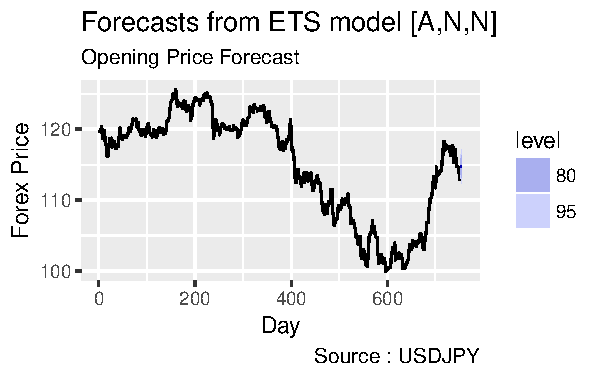
\includegraphics{binary-forex-trading-Q1_files/figure-latex/plotETS-1-1}
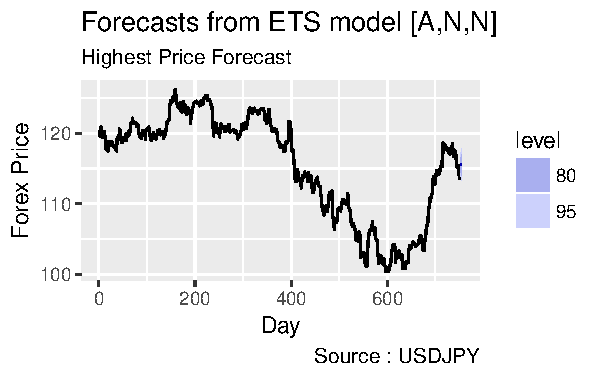
\includegraphics{binary-forex-trading-Q1_files/figure-latex/plotETS-1-2}
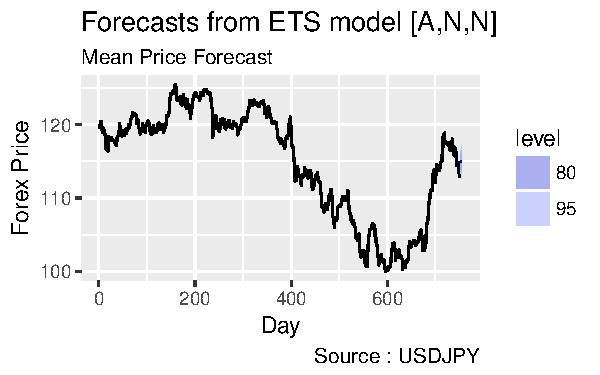
\includegraphics{binary-forex-trading-Q1_files/figure-latex/plotETS-1-3}
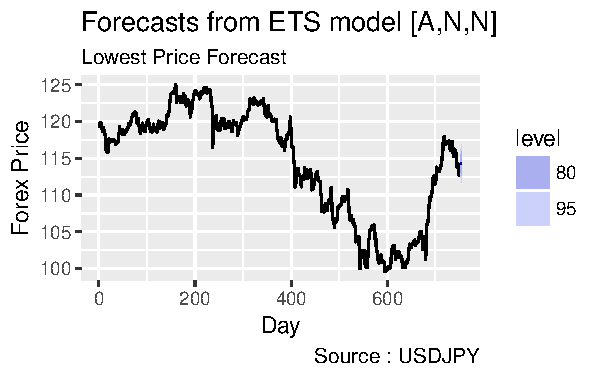
\includegraphics{binary-forex-trading-Q1_files/figure-latex/plotETS-1-4}
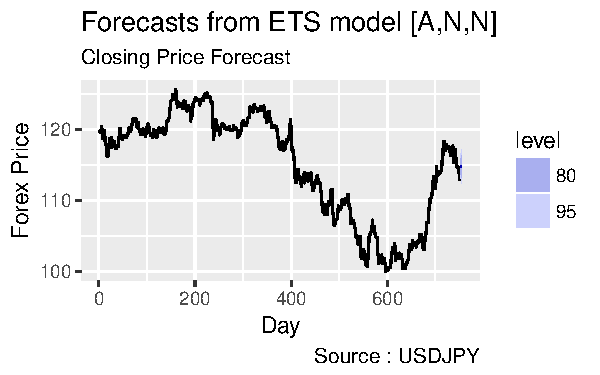
\includegraphics{binary-forex-trading-Q1_files/figure-latex/plotETS-1-5}

\includegraphics{binary-forex-trading-Q1_files/figure-latex/plotETS-2-1}

\subsubsection{2.1.3.2 Garch vs EWMA}\label{garch-vs-ewma-1}

\includegraphics{binary-forex-trading-Q1_files/figure-latex/plotGM-1-1}

\subsubsection{2.1.3.3 MCMC vs Bayesian Time
Series}\label{mcmc-vs-bayesian-time-series-1}

\subsubsection{2.1.3.4 MIDAS}\label{midas-1}

\subsection{2.1.4 Staking Model}\label{staking-model}

\subsubsection{2.1.4.1 ARIMA vs ETS}\label{arima-vs-ets-2}

Staking function. Here I apply Kelly criterion as the betting strategy.
I don't pretend to know the order of price flutuation flow from the
Hi-Lo price range, therefore I just using Closing price for settlement
while the staking price restricted within the variance (Hi-Lo) to made
the transaction stand. The settled price can only be closing price
unless staking price is opening price which sellable within the Hi-Lo
range.

Due to we cannot know the forecasted sell/buy price and also forecasted
closing price which is coming first solely from Hi-Lo data, therefore
the Profit\&Loss will slidely different (sell/buy price = forecasted
sell/buy price).

\begin{itemize}
\tightlist
\item
  Forecasted profit = edge based on forecasted sell/buy price -
  forecasted settled price.
\item
  If the forecasted sell/buy price doesn't exist within the Hi-Lo price,
  then the transaction is not stand.
\item
  If the forecasted settled price does not exist within the Hi-Lo price,
  then the settled price will be the real closing price.
\end{itemize}

Kindly refer to
\href{http://www.quintutive.com2012/08/22/arma-models-for-trading}{{\textbf{Quintuitive}
ARMA Models for Trading}} to know how to determine PULL or CALL with
ARMA models\footnote{The author compare the ROI between
  \textbf{Buy-and-Hold} with \textbf{GARCH} model.}.

Here I set an application of leverage while it is very risky (the
variance of ROI is very high) as we can know from later comparison.

\textbf{Staking Model}

For Buy-Low-Sell-High tactic, I placed two limit order for tomorrow now,
which are buy and sell. The transaction will be standed once the price
hit in tomorrow. If the buy price doesn't met, there will be no
transaction made, while sell price doesn't occur will use closing price
for settlement.\footnote{Using Kelly criterion staking model}

For variance betting, I used both focasted highest minus the forecasted
lowest price to get the range. After that placed two limit orders as
well. If one among the buy or sell price doesn't appear will use closing
price as final settlement.\footnote{Place \$100 for every single bet.}

\subsubsection{2.1.4.2 Garch vs EWMA}\label{garch-vs-ewma-2}

The staking models same with what I applied onto ETS modelled dataset.

\subsubsection{2.1.4.3 MCMC vs Bayesian Time
Series}\label{mcmc-vs-bayesian-time-series-2}

\subsubsection{2.1.4.4 MIDAS}\label{midas-2}

\subsection{2.1.5 Return of Investment}\label{return-of-investment}

\subsubsection{2.1.5.1 ARIMA vs ETS}\label{arima-vs-ets-3}

\begin{Shaded}
\begin{Highlighting}[]
\NormalTok{## load the pre-run and saved models.  Profit}
\NormalTok{## and Loss of Arima models.}

\NormalTok{flsAutoArima <-}\StringTok{ }\KeywordTok{dir}\NormalTok{(}\StringTok{"./data"}\NormalTok{, }\DataTypeTok{pattern =} \StringTok{"fundAutoArima"}\NormalTok{)}

\NormalTok{fundList <-}\StringTok{ }\KeywordTok{llply}\NormalTok{(flsAutoArima, }\ControlFlowTok{function}\NormalTok{(dt) \{}
    \KeywordTok{cbind}\NormalTok{(}\DataTypeTok{Model =} \KeywordTok{str_replace_all}\NormalTok{(dt, }\StringTok{".rds"}\NormalTok{, }
        \StringTok{""}\NormalTok{), }\KeywordTok{readRDS}\NormalTok{(}\DataTypeTok{file =} \KeywordTok{paste0}\NormalTok{(}\StringTok{"./data/"}\NormalTok{, }
\NormalTok{        dt))) }\OperatorTok\StringTok{ }\NormalTok{tbl_df}
\NormalTok{\})}
\KeywordTok{names}\NormalTok{(fundList) <-}\StringTok{ }\KeywordTok{sapply}\NormalTok{(fundList, }\ControlFlowTok{function}\NormalTok{(x) xts}\OperatorTok{::}\KeywordTok{first}\NormalTok{(x}\OperatorTok{$}\NormalTok{Model))}

\NormalTok{## Summary of ROI}
\NormalTok{aa.tbl <-}\StringTok{ }\KeywordTok{ldply}\NormalTok{(fundList, }\ControlFlowTok{function}\NormalTok{(x) \{}
\NormalTok{    x }\OperatorTok\StringTok{ }\KeywordTok{mutate}\NormalTok{(}\DataTypeTok{StartDate =}\NormalTok{ xts}\OperatorTok{::}\KeywordTok{first}\NormalTok{(Date), }
        \DataTypeTok{LatestDate =} \KeywordTok{last}\NormalTok{(Date), }\DataTypeTok{InitFund =}\NormalTok{ xts}\OperatorTok{::}\KeywordTok{first}\NormalTok{(BR), }
        \DataTypeTok{LatestFund =} \KeywordTok{last}\NormalTok{(Bal), }\DataTypeTok{Profit =} \KeywordTok{sum}\NormalTok{(Profit), }
        \DataTypeTok{RR =}\NormalTok{ LatestFund}\OperatorTok{/}\NormalTok{InitFund) }\OperatorTok\StringTok{ }\NormalTok{dplyr}\OperatorTok{::}\KeywordTok{select}\NormalTok{(StartDate, }
\NormalTok{        LatestDate, InitFund, LatestFund, Profit, }
\NormalTok{        RR) }\OperatorTok\StringTok{ }\NormalTok{unique}
\NormalTok{\}) }\OperatorTok\StringTok{ }\NormalTok{tbl_df}
\end{Highlighting}
\end{Shaded}

The return of investment from best fitted Auto Arima model.

\begin{verbatim}
 7 fundAutoArimaHILO 2015-01-02 2017-01-20     1000   1637.251 637.25113 1.637251
10 fundAutoArimaLOHI 2015-01-02 2017-01-20     1000   1716.985 716.98492 1.716985
\end{verbatim}

Profit and Loss of default \texttt{ZZZ} ets models.

\begin{Shaded}
\begin{Highlighting}[]
\NormalTok{## Model 1 without leverage.  Placed orders -}
\NormalTok{## Fund size without log}

\CommentTok{#'@ mbase <- USDJPY}

\NormalTok{## settled with highest price.}
\CommentTok{#'@ fundOPHI <- simStakesETS(mbase, .prCat = 'Op', .setPrice = 'Hi', .initialFundSize = 1000)}
\CommentTok{#'@ saveRDS(fundOPHI, file = './data/fundOPHI.rds')}

\CommentTok{#'@ fundHIHI <- simStakesETS(mbase, .prCat = 'Hi', .setPrice = 'Hi', .initialFundSize = 1000)}
\CommentTok{#'@ saveRDS(fundHIHI, file = './data/fundHIHI.rds')}

\CommentTok{#'@ fundMNHI <- simStakesETS(mbase, .prCat = 'Mn', .setPrice = 'Hi', .initialFundSize = 1000)}
\CommentTok{#'@ saveRDS(fundMNHI, file = './data/fundMNHI.rds')}

\CommentTok{#'@ fundLOHI <- simStakesETS(mbase, .prCat = 'Lo', .setPrice = 'Hi', .initialFundSize = 1000)}
\CommentTok{#'@ saveRDS(fundLOHI, file = './data/fundLOHI.rds')}

\CommentTok{#'@ fundCLHI <- simStakesETS(mbase, .prCat = 'Cl', .setPrice = 'Hi', .initialFundSize = 1000)}
\CommentTok{#'@ saveRDS(fundCLHI, file = './data/fundCLHI.rds')}


\NormalTok{## settled with mean price.}
\CommentTok{#'@ fundOPMN <- simStakesETS(mbase, .prCat = 'Op', .setPrice = 'Mn', .initialFundSize = 1000)}
\CommentTok{#'@ saveRDS(fundOPMN, file = './data/fundOPMN.rds')}

\CommentTok{#'@ fundHIMN <- simStakesETS(mbase, .prCat = 'Hi', .setPrice = 'Mn', .initialFundSize = 1000)}
\CommentTok{#'@ saveRDS(fundHIMN, file = './data/fundHIMN.rds')}

\CommentTok{#'@ fundMNMN <- simStakesETS(mbase, .prCat = 'Mn', .setPrice = 'Mn', .initialFundSize = 1000)}
\CommentTok{#'@ saveRDS(fundMNMN, file = './data/fundMNMN.rds')}

\CommentTok{#'@ fundLOMN <- simStakesETS(mbase, .prCat = 'Lo', .setPrice = 'Mn', .initialFundSize = 1000)}
\CommentTok{#'@ saveRDS(fundLOMN, file = './data/fundLOMN.rds')}

\CommentTok{#'@ fundCLMN <- simStakesETS(mbase, .prCat = 'Cl', .setPrice = 'Mn', .initialFundSize = 1000)}
\CommentTok{#'@ saveRDS(fundCLMN, file = './data/fundCLMN.rds')}


\NormalTok{## settled with opening price.}
\CommentTok{#'@ fundOPLO <- simStakesETS(mbase, .prCat = 'Op', .setPrice = 'Lo', .initialFundSize = 1000)}
\CommentTok{#'@ saveRDS(fundOPLO, file = './data/fundOPLO.rds')}

\CommentTok{#'@ fundHILO <- simStakesETS(mbase, .prCat = 'Hi', .setPrice = 'Lo', .initialFundSize = 1000)}
\CommentTok{#'@ saveRDS(fundHILO, file = './data/fundHILO.rds')}

\CommentTok{#'@ fundMNLO <- simStakesETS(mbase, .prCat = 'Mn', .setPrice = 'Lo', .initialFundSize = 1000)}
\CommentTok{#'@ saveRDS(fundMNLO, file = './data/fundMNLO.rds')}

\CommentTok{#'@ fundLOLO <- simStakesETS(mbase, .prCat = 'Lo', .setPrice = 'Lo', .initialFundSize = 1000)}
\CommentTok{#'@ saveRDS(fundLOLO, file = './data/fundLOLO.rds')}

\CommentTok{#'@ fundCLLO <- simStakesETS(mbase, .prCat = 'Cl', .setPrice = 'Lo', .initialFundSize = 1000)}
\CommentTok{#'@ saveRDS(fundCLLO, file = './data/fundCLLO.rds')}


\NormalTok{## settled with closing price.}
\CommentTok{#'@ fundOPCL <- simStakesETS(mbase, .prCat = 'Op', .setPrice = 'Cl', .initialFundSize = 1000)}
\CommentTok{#'@ saveRDS(fundOPCL, file = './data/fundOPCL.rds')}

\CommentTok{#'@ fundHICL <- simStakesETS(mbase, .prCat = 'Hi', .setPrice = 'Cl', .initialFundSize = 1000)}
\CommentTok{#'@ saveRDS(fundHICL, file = './data/fundHICL.rds')}

\CommentTok{#'@ fundMNCL <- simStakesETS(mbase, .prCat = 'Mn', .setPrice = 'Cl', .initialFundSize = 1000)}
\CommentTok{#'@ saveRDS(fundMNCL, file = './data/fundMNCL.rds')}

\CommentTok{#'@ fundLOCL <- simStakesETS(mbase, .prCat = 'Lo', .setPrice = 'Cl', .initialFundSize = 1000)}
\CommentTok{#'@ saveRDS(fundLOCL, file = './data/fundLOCL.rds')}

\CommentTok{#'@ fundCLCL <- simStakesETS(mbase, .prCat = 'Cl', .setPrice = 'Cl', .initialFundSize = 1000)}
\CommentTok{#'@ saveRDS(fundCLCL, file = './data/fundCLCL.rds')}

\NormalTok{## Placed orders - Fund size without log}
\CommentTok{#'@ fundList <- list(fundOPHI = fundOPHI, fundHIHI = fundHIHI, fundMNHI = fundMNHI, fundLOHI = fundLOHI, fundCLHI = fundCLHI, }
\CommentTok{#'@                 fundOPMN = fundOPMN, fundHIMN = fundHIMN, fundMNMN = fundMNMN, fundLOMN = fundLOMN, fundCLMN = fundCLMN, }
\CommentTok{#'@                 fundOPLO = fundOPLO, fundHILO = fundHILO, fundMNLO = fundMNLO, fundLOLO = fundLOLO, fundCLLO = fundCLLO, }
\CommentTok{#'@                 fundOPCL = fundOPCL, fundHICL = fundHICL, fundMNCL = fundMNCL, fundLOCL = fundLOCL, fundCLCL = fundCLCL)}

\CommentTok{#'@ ldply(fundList, function(x) \{ x %>% mutate(StartDate = first(Date), LatestDate = last(Date), InitFund = first(BR), LatestFund = last(Bal), Profit = sum(Profit), RR = LatestFund/InitFund) %>% dplyr::select(StartDate, LatestDate, InitFund, LatestFund, Profit, RR) %>% unique \}) %>% tbl_df}
\NormalTok{## A tibble: 20 × 5 .id StartDate LatestDate}
\NormalTok{## InitFund LatestFund Profit RR <chr> <date>}
\NormalTok{## <date> <dbl> <dbl> <dbl> <dbl> 1 fundOPHI}
\NormalTok{## 2015-01-02 2017-01-20 1000 326.83685}
\NormalTok{## 1326.837 1.326837 2 fundHIHI 2015-01-02}
\NormalTok{## 2017-01-20 1000 0.00000 1000.000 1.000000 3}
\NormalTok{## fundMNHI 2015-01-02 2017-01-20 1000}
\NormalTok{## 152.30210 1152.302 1.152302 4 fundLOHI}
\NormalTok{## 2015-01-02 2017-01-20 1000 816.63808}
\NormalTok{## 1816.638 1.816638 5 fundCLHI 2015-01-02}
\NormalTok{## 2017-01-20 1000 323.18564 1323.186 1.323186}
\NormalTok{## 6 fundOPMN 2015-01-02 2017-01-20 1000}
\NormalTok{## 246.68001 1246.680 1.246680 7 fundHIMN}
\NormalTok{## 2015-01-02 2017-01-20 1000 384.90915}
\NormalTok{## 1384.909 1.384909 8 fundMNMN 2015-01-02}
\NormalTok{## 2017-01-20 1000 0.00000 1000.000 1.000000 9}
\NormalTok{## fundLOMN 2015-01-02 2017-01-20 1000}
\NormalTok{## 529.34170 1529.342 1.529342 10 fundCLMN}
\NormalTok{## 2015-01-02 2017-01-20 1000 221.03926}
\NormalTok{## 1221.039 1.221039 11 fundOPLO 2015-01-02}
\NormalTok{## 2017-01-20 1000 268.31155 1268.312 1.268312}
\NormalTok{## 12 fundHILO 2015-01-02 2017-01-20 1000}
\NormalTok{## 649.35074 1649.351 1.649351 13 fundMNLO}
\NormalTok{## 2015-01-02 2017-01-20 1000 298.28509}
\NormalTok{## 1298.285 1.298285 14 fundLOLO 2015-01-02}
\NormalTok{## 2017-01-20 1000 0.00000 1000.000 1.000000 15}
\NormalTok{## fundCLLO 2015-01-02 2017-01-20 1000}
\NormalTok{## 208.85690 1208.857 1.208857 16 fundOPCL}
\NormalTok{## 2015-01-02 2017-01-20 1000 30.55969 1030.560}
\NormalTok{## 1.030560 17 fundHICL 2015-01-02 2017-01-20}
\NormalTok{## 1000 400.59057 1400.591 1.400591 18 fundMNCL}
\NormalTok{## 2015-01-02 2017-01-20 1000 117.96808}
\NormalTok{## 1117.968 1.117968 19 fundLOCL 2015-01-02}
\NormalTok{## 2017-01-20 1000 530.68975 1530.690 1.530690}
\NormalTok{## 20 fundCLCL 2015-01-02 2017-01-20 1000}
\NormalTok{## 0.00000 1000.000 1.000000}

\NormalTok{## load fund files which is from chunk `r}
\NormalTok{## simStaking-woutLog`.}
\NormalTok{fundOPHI <-}\StringTok{ }\KeywordTok{readRDS}\NormalTok{(}\StringTok{"./data/fundOPHI.rds"}\NormalTok{)}
\NormalTok{fundHIHI <-}\StringTok{ }\KeywordTok{readRDS}\NormalTok{(}\StringTok{"./data/fundHIHI.rds"}\NormalTok{)}
\NormalTok{fundMNHI <-}\StringTok{ }\KeywordTok{readRDS}\NormalTok{(}\StringTok{"./data/fundMNHI.rds"}\NormalTok{)}
\NormalTok{fundLOHI <-}\StringTok{ }\KeywordTok{readRDS}\NormalTok{(}\StringTok{"./data/fundLOHI.rds"}\NormalTok{)}
\NormalTok{fundCLHI <-}\StringTok{ }\KeywordTok{readRDS}\NormalTok{(}\StringTok{"./data/fundCLHI.rds"}\NormalTok{)}
\NormalTok{fundOPMN <-}\StringTok{ }\KeywordTok{readRDS}\NormalTok{(}\StringTok{"./data/fundOPMN.rds"}\NormalTok{)}
\NormalTok{fundHIMN <-}\StringTok{ }\KeywordTok{readRDS}\NormalTok{(}\StringTok{"./data/fundHIMN.rds"}\NormalTok{)}
\NormalTok{fundMNMN <-}\StringTok{ }\KeywordTok{readRDS}\NormalTok{(}\StringTok{"./data/fundMNMN.rds"}\NormalTok{)}
\NormalTok{fundLOMN <-}\StringTok{ }\KeywordTok{readRDS}\NormalTok{(}\StringTok{"./data/fundLOMN.rds"}\NormalTok{)}
\NormalTok{fundCLMN <-}\StringTok{ }\KeywordTok{readRDS}\NormalTok{(}\StringTok{"./data/fundCLMN.rds"}\NormalTok{)}
\NormalTok{fundOPLO <-}\StringTok{ }\KeywordTok{readRDS}\NormalTok{(}\StringTok{"./data/fundOPLO.rds"}\NormalTok{)}
\NormalTok{fundHILO <-}\StringTok{ }\KeywordTok{readRDS}\NormalTok{(}\StringTok{"./data/fundHILO.rds"}\NormalTok{)}
\NormalTok{fundMNLO <-}\StringTok{ }\KeywordTok{readRDS}\NormalTok{(}\StringTok{"./data/fundMNLO.rds"}\NormalTok{)}
\NormalTok{fundLOLO <-}\StringTok{ }\KeywordTok{readRDS}\NormalTok{(}\StringTok{"./data/fundLOLO.rds"}\NormalTok{)}
\NormalTok{fundCLLO <-}\StringTok{ }\KeywordTok{readRDS}\NormalTok{(}\StringTok{"./data/fundCLLO.rds"}\NormalTok{)}
\NormalTok{fundOPCL <-}\StringTok{ }\KeywordTok{readRDS}\NormalTok{(}\StringTok{"./data/fundOPCL.rds"}\NormalTok{)}
\NormalTok{fundHICL <-}\StringTok{ }\KeywordTok{readRDS}\NormalTok{(}\StringTok{"./data/fundHICL.rds"}\NormalTok{)}
\NormalTok{fundMNCL <-}\StringTok{ }\KeywordTok{readRDS}\NormalTok{(}\StringTok{"./data/fundMNCL.rds"}\NormalTok{)}
\NormalTok{fundLOCL <-}\StringTok{ }\KeywordTok{readRDS}\NormalTok{(}\StringTok{"./data/fundLOCL.rds"}\NormalTok{)}
\NormalTok{fundCLCL <-}\StringTok{ }\KeywordTok{readRDS}\NormalTok{(}\StringTok{"./data/fundCLCL.rds"}\NormalTok{)}

\NormalTok{## Placed orders - Fund size without log}
\NormalTok{fundList <-}\StringTok{ }\KeywordTok{list}\NormalTok{(}\DataTypeTok{fundOPHI =}\NormalTok{ fundOPHI, }\DataTypeTok{fundHIHI =}\NormalTok{ fundHIHI, }
    \DataTypeTok{fundMNHI =}\NormalTok{ fundMNHI, }\DataTypeTok{fundLOHI =}\NormalTok{ fundLOHI, }
    \DataTypeTok{fundCLHI =}\NormalTok{ fundCLHI, }\DataTypeTok{fundOPMN =}\NormalTok{ fundOPMN, }
    \DataTypeTok{fundHIMN =}\NormalTok{ fundHIMN, }\DataTypeTok{fundMNMN =}\NormalTok{ fundMNMN, }
    \DataTypeTok{fundLOMN =}\NormalTok{ fundLOMN, }\DataTypeTok{fundCLMN =}\NormalTok{ fundCLMN, }
    \DataTypeTok{fundOPLO =}\NormalTok{ fundOPLO, }\DataTypeTok{fundHILO =}\NormalTok{ fundHILO, }
    \DataTypeTok{fundMNLO =}\NormalTok{ fundMNLO, }\DataTypeTok{fundLOLO =}\NormalTok{ fundLOLO, }
    \DataTypeTok{fundCLLO =}\NormalTok{ fundCLLO, }\DataTypeTok{fundOPCL =}\NormalTok{ fundOPCL, }
    \DataTypeTok{fundHICL =}\NormalTok{ fundHICL, }\DataTypeTok{fundMNCL =}\NormalTok{ fundMNCL, }
    \DataTypeTok{fundLOCL =}\NormalTok{ fundLOCL, }\DataTypeTok{fundCLCL =}\NormalTok{ fundCLCL)}
\end{Highlighting}
\end{Shaded}

From above table summary we can know that
\texttt{model\ 1\ without\ any\ leverage} will be growth with a stable
pace where LoHi and LoHi generates highest return rates. fundLOHI
indicates investment \textbf{fund} buy at \textbf{LO}west price and sell
at \textbf{HI}ghest price and vice verse.

\begin{verbatim}
# 4  fundLOHI 2015-01-02 2017-01-20      1000  816.63808   1816.638  1.816638
#12  fundHILO 2015-01-02 2017-01-20      1000  649.35074   1649.351  1.649351
\end{verbatim}

\subsubsection{2.1.5.2 Garch vs EWMA}\label{garch-vs-ewma-3}

From above table summary we can know that
\texttt{model\ 1\ without\ any\ leverage} will be growth with a stable
pace where LoHi and LoHi generates highest return rates. fundLOHI
indicates investment \textbf{fund} buy at \textbf{LO}west price and sell
at \textbf{HI}ghest price and vice verse.

\begin{verbatim}
# 4  fundGMLOHI 2015-01-02 2017-01-20     1000   1770.291 7.702907e+02 1.770291
#12  fundGMHILO 2015-01-02 2017-01-20     1000   1713.915 7.139146e+02 1.713915
\end{verbatim}

\subsubsection{2.1.5.3 MCMC vs Bayesian Time
Series}\label{mcmc-vs-bayesian-time-series-3}

\subsubsection{2.1.5.4 MIDAS}\label{midas-3}

\subsection{2.1.6 Return of Investment
Optimization}\label{return-of-investment-optimization}

\subsubsection{2.1.6.1 ARIMA vs ETS}\label{arima-vs-ets-4}

Now we apply the bootstrap (Application of Monte Carlo method to
simulate 10000 times) onto the simulation of the forecasting.

\begin{Shaded}
\begin{Highlighting}[]
\NormalTok{## set all models provided by ets function.}
\NormalTok{ets.m1 <-}\StringTok{ }\KeywordTok{c}\NormalTok{(}\StringTok{"A"}\NormalTok{, }\StringTok{"M"}\NormalTok{, }\StringTok{"Z"}\NormalTok{)}
\NormalTok{ets.m2 <-}\StringTok{ }\KeywordTok{c}\NormalTok{(}\StringTok{"N"}\NormalTok{, }\StringTok{"A"}\NormalTok{, }\StringTok{"M"}\NormalTok{, }\StringTok{"Z"}\NormalTok{)}
\NormalTok{ets.m3 <-}\StringTok{ }\KeywordTok{c}\NormalTok{(}\StringTok{"N"}\NormalTok{, }\StringTok{"A"}\NormalTok{, }\StringTok{"M"}\NormalTok{, }\StringTok{"Z"}\NormalTok{)}
\NormalTok{ets.m <-}\StringTok{ }\KeywordTok{do.call}\NormalTok{(paste0, }\KeywordTok{expand.grid}\NormalTok{(ets.m1, ets.m2, }
\NormalTok{    ets.m3))}
\KeywordTok{rm}\NormalTok{(ets.m1, ets.m2, ets.m3)}

\NormalTok{pp <-}\StringTok{ }\KeywordTok{expand.grid}\NormalTok{(}\KeywordTok{c}\NormalTok{(}\StringTok{"Op"}\NormalTok{, }\StringTok{"Hi"}\NormalTok{, }\StringTok{"Mn"}\NormalTok{, }\StringTok{"Lo"}\NormalTok{, }\StringTok{"Cl"}\NormalTok{), }
    \KeywordTok{c}\NormalTok{(}\StringTok{"Op"}\NormalTok{, }\StringTok{"Hi"}\NormalTok{, }\StringTok{"Mn"}\NormalTok{, }\StringTok{"Lo"}\NormalTok{, }\StringTok{"Cl"}\NormalTok{)) }\OperatorTok\StringTok{ }\KeywordTok{mutate}\NormalTok{(}\DataTypeTok{PP =} \KeywordTok{paste}\NormalTok{(Var1, }
\NormalTok{    Var2)) }\OperatorTok\StringTok{ }\NormalTok{.}\OperatorTok{$}\NormalTok{PP }\OperatorTok\StringTok{ }\KeywordTok{str_split}\NormalTok{(}\StringTok{" "}\NormalTok{)}
\end{Highlighting}
\end{Shaded}

In order to trace the errors, here I check the source codes of the
function but also test the coding as you can know via
\href{https://github.com/robjhyndman/forecast/issues/554}{{Error :
Forbidden model combination \#554}}. Here I only take 22 models among 48
models.

\begin{Shaded}
\begin{Highlighting}[]
\NormalTok{## load the pre-run and saved models.  Profit}
\NormalTok{## and Loss of multi-ets models. 22 models.}

\NormalTok{## Due to the file name contains 'MNM' is not}
\NormalTok{## found in directory but appear in dir(), Here}
\NormalTok{## I force to omit it...}
\CommentTok{#' @> sapply(ets.m, function(x) \{ }
\CommentTok{#' @     dir('data', pattern = x) %>% length}
\CommentTok{#' @ \}, USE.NAMES = TRUE) %>% .[. > 0]}
\CommentTok{# ANN MNN ZNN AAN MAN ZAN MMN ZMN AZN MZN ZZN}
\CommentTok{# MNM ANZ MNZ ZNZ AAZ MAZ ZAZ MMZ ZMZ AZZ MZZ}
\CommentTok{# ZZZ 25 25 25 25 25 25 25 25 25 25 25 1 25 25}
\CommentTok{# 25 25 25 25 25 25 25 25 25}

\NormalTok{nms <-}\StringTok{ }\KeywordTok{sapply}\NormalTok{(ets.m, }\ControlFlowTok{function}\NormalTok{(x) \{}
    \KeywordTok{dir}\NormalTok{(}\StringTok{"data"}\NormalTok{, }\DataTypeTok{pattern =}\NormalTok{ x) }\OperatorTok\StringTok{ }\NormalTok{length}
\NormalTok{\}, }\DataTypeTok{USE.NAMES =} \OtherTok{TRUE}\NormalTok{) }\OperatorTok\StringTok{ }\NormalTok{.[. }\OperatorTok{==}\StringTok{ }\DecValTok{25}\NormalTok{] }\OperatorTok\StringTok{ }\NormalTok{names  }\CommentTok{#here I use only [. == 25].}


\CommentTok{#'@ nms <- sapply(ets.m, function(x) \{ }
\CommentTok{#'@    dir('data', pattern = x) %>% length}
\CommentTok{#'@  \}, USE.NAMES = TRUE) %>% .[. > 0] %>% names #here original [. > 0].}

\NormalTok{fls <-}\StringTok{ }\KeywordTok{sapply}\NormalTok{(nms, }\ControlFlowTok{function}\NormalTok{(x) \{}
    \KeywordTok{sapply}\NormalTok{(pp, }\ControlFlowTok{function}\NormalTok{(y) \{}
        \KeywordTok{dir}\NormalTok{(}\StringTok{"data"}\NormalTok{, }\DataTypeTok{pattern =} \KeywordTok{paste0}\NormalTok{(x, }\StringTok{"."}\NormalTok{, y[}\DecValTok{1}\NormalTok{], }
\NormalTok{            y[}\DecValTok{2}\NormalTok{]))}
\NormalTok{    \})}
\NormalTok{\})}

\NormalTok{## From 22 ets models with 25 hilo, opcl, mnmn,}
\NormalTok{## opop etc different price data. There will be}
\NormalTok{## 550 models.}
\NormalTok{fundList <-}\StringTok{ }\KeywordTok{llply}\NormalTok{(fls, }\ControlFlowTok{function}\NormalTok{(dt) \{}
    \KeywordTok{cbind}\NormalTok{(}\DataTypeTok{Model =} \KeywordTok{str_replace_all}\NormalTok{(dt, }\StringTok{".rds"}\NormalTok{, }
        \StringTok{""}\NormalTok{), }\KeywordTok{readRDS}\NormalTok{(}\DataTypeTok{file =} \KeywordTok{paste0}\NormalTok{(}\StringTok{"./data/"}\NormalTok{, }
\NormalTok{        dt))) }\OperatorTok\StringTok{ }\NormalTok{tbl_df}
\NormalTok{\})}
\KeywordTok{names}\NormalTok{(fundList) <-}\StringTok{ }\KeywordTok{sapply}\NormalTok{(fundList, }\ControlFlowTok{function}\NormalTok{(x) xts}\OperatorTok{::}\KeywordTok{first}\NormalTok{(x}\OperatorTok{$}\NormalTok{Model))}

\NormalTok{## Summary of ROI}
\NormalTok{ets.tbl <-}\StringTok{ }\KeywordTok{ldply}\NormalTok{(fundList, }\ControlFlowTok{function}\NormalTok{(x) \{}
\NormalTok{    x }\OperatorTok\StringTok{ }\KeywordTok{mutate}\NormalTok{(}\DataTypeTok{StartDate =}\NormalTok{ xts}\OperatorTok{::}\KeywordTok{first}\NormalTok{(Date), }
        \DataTypeTok{LatestDate =} \KeywordTok{last}\NormalTok{(Date), }\DataTypeTok{InitFund =}\NormalTok{ xts}\OperatorTok{::}\KeywordTok{first}\NormalTok{(BR), }
        \DataTypeTok{LatestFund =} \KeywordTok{last}\NormalTok{(Bal), }\DataTypeTok{Profit =} \KeywordTok{sum}\NormalTok{(Profit), }
        \DataTypeTok{RR =}\NormalTok{ LatestFund}\OperatorTok{/}\NormalTok{InitFund) }\OperatorTok\StringTok{ }\NormalTok{dplyr}\OperatorTok{::}\KeywordTok{select}\NormalTok{(StartDate, }
\NormalTok{        LatestDate, InitFund, LatestFund, Profit, }
\NormalTok{        RR) }\OperatorTok\StringTok{ }\NormalTok{unique}
\NormalTok{\}) }\OperatorTok\StringTok{ }\NormalTok{tbl_df}
\end{Highlighting}
\end{Shaded}

\includegraphics{binary-forex-trading-Q1_files/figure-latex/plot-ets2-1}

\begin{Shaded}
\begin{Highlighting}[]
\CommentTok{#'@ ets.tbl %>% dplyr::filter(RR == max(RR))}
\CommentTok{# A tibble: 2 x 7 .id StartDate LatestDate}
\CommentTok{# InitFund LatestFund Profit RR <chr> <date>}
\CommentTok{# <date> <dbl> <dbl> <dbl> <dbl> 1 AZN.LoHi}
\CommentTok{# 2015-01-02 2017-01-20 1000 1834.058 834.058}
\CommentTok{# 1.834058 2 AZZ.LoHi 2015-01-02 2017-01-20}
\CommentTok{# 1000 1834.058 834.058 1.834058}

\KeywordTok{ldply}\NormalTok{(}\KeywordTok{c}\NormalTok{(}\StringTok{"LoHi"}\NormalTok{, }\StringTok{"HiLo"}\NormalTok{), }\ControlFlowTok{function}\NormalTok{(ppr) \{}
\NormalTok{    ets.tbl }\OperatorTok\StringTok{ }\NormalTok{dplyr}\OperatorTok{::}\KeywordTok{filter}\NormalTok{(.id }\OperatorTok\StringTok{ }\KeywordTok{grep}\NormalTok{(ppr, }
\NormalTok{        ets.tbl}\OperatorTok{$}\NormalTok{.id, }\DataTypeTok{value =} \OtherTok{TRUE}\NormalTok{)) }\OperatorTok\StringTok{ }\NormalTok{dplyr}\OperatorTok{::}\KeywordTok{filter}\NormalTok{(RR }\OperatorTok{==}\StringTok{ }
\StringTok{        }\KeywordTok{max}\NormalTok{(RR)) }\OperatorTok\StringTok{ }\NormalTok{unique}
\NormalTok{\})}
\end{Highlighting}
\end{Shaded}

\begin{verbatim}
##        .id  StartDate LatestDate InitFund
## 1 AZN.LoHi 2015-01-02 2017-01-20     1000
## 2 AZZ.LoHi 2015-01-02 2017-01-20     1000
## 3 AZN.HiLo 2015-01-02 2017-01-20     1000
## 4 AZZ.HiLo 2015-01-02 2017-01-20     1000
##   LatestFund   Profit       RR
## 1   1834.058 834.0580 1.834058
## 2   1834.058 834.0580 1.834058
## 3   1666.752 666.7518 1.666752
## 4   1666.752 666.7518 1.666752
\end{verbatim}

\begin{Shaded}
\begin{Highlighting}[]
\CommentTok{# A tibble: 4 x 7 .id StartDate LatestDate}
\CommentTok{# InitFund LatestFund Profit RR <chr> <date>}
\CommentTok{# <date> <dbl> <dbl> <dbl> <dbl> 1 AZN.LoHi}
\CommentTok{# 2015-01-02 2017-01-20 1000 1834.058 834.0580}
\CommentTok{# 1.834058 2 AZZ.LoHi 2015-01-02 2017-01-20}
\CommentTok{# 1000 1834.058 834.0580 1.834058 3 AZN.HiLo}
\CommentTok{# 2015-01-02 2017-01-20 1000 1666.752 666.7518}
\CommentTok{# 1.666752 4 AZZ.HiLo 2015-01-02 2017-01-20}
\CommentTok{# 1000 1666.752 666.7518 1.666752}
\end{Highlighting}
\end{Shaded}

From above table, we find the ets model \texttt{AZN} and \texttt{AZZ}
generates highest return compare to rest of 21 ets models.

\emph{Figlewski (2004)} applied few models and also using different
length of data for comparison. Now I use daily Hi-Lo and 365 days data
in order to predict the next market price. Since I only predict 2 years
investment therefore a further research works on the data sizing and
longer prediction terms need (for example: 1 month, 3 months, 6 months
data to predict coming price, 2ndly comparison of the ROI from 7 years
or upper).

\textbf{Variance/Volatility Analsis}

Hereby, I try to place bets on the variance which is requested by the
assessment. Firstly we look at \textbf{Auto Arima} model.

\begin{Shaded}
\begin{Highlighting}[]
\NormalTok{## load the pre-run and saved models.  Profit}
\NormalTok{## and Loss of Arima models.}

\NormalTok{fundList <-}\StringTok{ }\KeywordTok{llply}\NormalTok{(flsAutoArima, }\ControlFlowTok{function}\NormalTok{(dt) \{}
    \KeywordTok{cbind}\NormalTok{(}\DataTypeTok{Model =} \KeywordTok{str_replace_all}\NormalTok{(dt, }\StringTok{".rds"}\NormalTok{, }
        \StringTok{""}\NormalTok{), }\KeywordTok{readRDS}\NormalTok{(}\DataTypeTok{file =} \KeywordTok{paste0}\NormalTok{(}\StringTok{"./data/"}\NormalTok{, }
\NormalTok{        dt))) }\OperatorTok\StringTok{ }\NormalTok{tbl_df}
\NormalTok{\})}
\KeywordTok{names}\NormalTok{(fundList) <-}\StringTok{ }\KeywordTok{sapply}\NormalTok{(fundList, }\ControlFlowTok{function}\NormalTok{(x) xts}\OperatorTok{::}\KeywordTok{first}\NormalTok{(x}\OperatorTok{$}\NormalTok{Model))}
\end{Highlighting}
\end{Shaded}

\begin{Shaded}
\begin{Highlighting}[]
\NormalTok{## Focast the variance and convert to}
\NormalTok{## probability.}
\NormalTok{varHL <-}\StringTok{ }\NormalTok{fundList[}\KeywordTok{grep}\NormalTok{(}\StringTok{"HILO|LOHI"}\NormalTok{, }\KeywordTok{names}\NormalTok{(fundList))]}
\NormalTok{ntm <-}\StringTok{ }\KeywordTok{c}\NormalTok{(}\KeywordTok{names}\NormalTok{((varHL)[}\KeywordTok{names}\NormalTok{(varHL) }\OperatorTok\StringTok{ }\KeywordTok{c}\NormalTok{(}\StringTok{"Date"}\NormalTok{, }
    \StringTok{"USDJPY.High"}\NormalTok{, }\StringTok{"USDJPY.Low"}\NormalTok{, }\StringTok{"USDJPY.Close"}\NormalTok{)]), }
    \KeywordTok{names}\NormalTok{((varHL)[}\OperatorTok{!}\KeywordTok{names}\NormalTok{(varHL) }\OperatorTok\StringTok{ }\KeywordTok{c}\NormalTok{(}\StringTok{"Date"}\NormalTok{, }
        \StringTok{"USDJPY.High"}\NormalTok{, }\StringTok{"USDJPY.Low"}\NormalTok{, }\StringTok{"USDJPY.Close"}\NormalTok{)])) }\OperatorTok\StringTok{ }
\StringTok{    }\KeywordTok{str_replace}\NormalTok{(}\StringTok{".HILO|.LOHI"}\NormalTok{, }\StringTok{""}\NormalTok{) }\OperatorTok\StringTok{ }\NormalTok{unique }\OperatorTok\StringTok{ }
\StringTok{    }\NormalTok{sort}

\NormalTok{varHL1 <-}\StringTok{ }\KeywordTok{suppressMessages}\NormalTok{(}\KeywordTok{llply}\NormalTok{(varHL, }\ControlFlowTok{function}\NormalTok{(dtx) \{}
\NormalTok{    mm =}\StringTok{ }\KeywordTok{tbl_df}\NormalTok{(dtx) }\OperatorTok\StringTok{ }\NormalTok{dplyr}\OperatorTok{::}\KeywordTok{select}\NormalTok{(Date, USDJPY.High, }
\NormalTok{        USDJPY.Low, USDJPY.Close, Point.Forecast)}
    \KeywordTok{names}\NormalTok{(mm)[}\DecValTok{5}\NormalTok{] =}\StringTok{ }\KeywordTok{as.character}\NormalTok{(dtx}\OperatorTok{$}\NormalTok{Model[}\DecValTok{1}\NormalTok{])}
    \KeywordTok{names}\NormalTok{(mm) =}\StringTok{ }\KeywordTok{str_replace_all}\NormalTok{(}\KeywordTok{names}\NormalTok{(mm), }\StringTok{"HiLo"}\NormalTok{, }
        \StringTok{"High"}\NormalTok{)}
    \KeywordTok{names}\NormalTok{(mm) =}\StringTok{ }\KeywordTok{str_replace_all}\NormalTok{(}\KeywordTok{names}\NormalTok{(mm), }\StringTok{"LoHi"}\NormalTok{, }
        \StringTok{"Low"}\NormalTok{)}
\NormalTok{    mm}
\NormalTok{\}) }\OperatorTok\StringTok{ }\NormalTok{join_all) }\OperatorTok\StringTok{ }\NormalTok{tbl_df}

\NormalTok{varHL2 <-}\StringTok{ }\KeywordTok{suppressMessages}\NormalTok{(}\KeywordTok{llply}\NormalTok{(ntm, }\ControlFlowTok{function}\NormalTok{(nm) \{}
\NormalTok{    mld =}\StringTok{ }\NormalTok{varHL1[}\KeywordTok{grep}\NormalTok{(nm, }\KeywordTok{names}\NormalTok{(varHL1))]}
\NormalTok{    mld[, }\DecValTok{3}\NormalTok{] =}\StringTok{ }\KeywordTok{abs}\NormalTok{(mld[, }\DecValTok{1}\NormalTok{] }\OperatorTok{-}\StringTok{ }\NormalTok{mld[, }\DecValTok{2}\NormalTok{])}
    \KeywordTok{names}\NormalTok{(mld)[}\DecValTok{3}\NormalTok{] =}\StringTok{ }\KeywordTok{paste0}\NormalTok{(nm, }\StringTok{".Rng"}\NormalTok{)}
\NormalTok{    mld =}\StringTok{ }\NormalTok{mld[}\KeywordTok{colSums}\NormalTok{(}\OperatorTok{!}\KeywordTok{is.na}\NormalTok{(mld)) }\OperatorTok{>}\StringTok{ }\DecValTok{0}\NormalTok{]}
    \KeywordTok{data.frame}\NormalTok{(varHL1[}\KeywordTok{c}\NormalTok{(}\StringTok{"Date"}\NormalTok{, }\StringTok{"USDJPY.High"}\NormalTok{, }
        \StringTok{"USDJPY.Low"}\NormalTok{, }\StringTok{"USDJPY.Close"}\NormalTok{)], }\DataTypeTok{USDJPY.Rng =} \KeywordTok{abs}\NormalTok{(varHL1}\OperatorTok{$}\NormalTok{USDJPY.High }\OperatorTok{-}\StringTok{ }
\StringTok{        }\NormalTok{varHL1}\OperatorTok{$}\NormalTok{USDJPY.Low), mld) }\OperatorTok\StringTok{ }\NormalTok{tbl_df}
\NormalTok{\}) }\OperatorTok\StringTok{ }\NormalTok{unique }\OperatorTok\StringTok{ }\NormalTok{join_all }\OperatorTok\StringTok{ }\NormalTok{tbl_df)}
\end{Highlighting}
\end{Shaded}

\begin{Shaded}
\begin{Highlighting}[]
\NormalTok{## Application of MASS::mvrnorm() or}
\NormalTok{## mvtnorm::rmvnorm() ##nope}
\CommentTok{#'@ varHL2 <- xts(varHL2[, -1], as.Date(varHL2$Date))}

\NormalTok{## Betting strategy 1 - Normal range betting}
\NormalTok{varB1 <-}\StringTok{ }\NormalTok{varHL2[, }\KeywordTok{c}\NormalTok{(}\StringTok{"Date"}\NormalTok{, }\KeywordTok{names}\NormalTok{(varHL2)[}\KeywordTok{str_detect}\NormalTok{(}\KeywordTok{names}\NormalTok{(varHL2), }
    \StringTok{".Rng"}\NormalTok{)])]}

\NormalTok{varB1 <-}\StringTok{ }\KeywordTok{suppressMessages}\NormalTok{(}\KeywordTok{llply}\NormalTok{(ntm, }\ControlFlowTok{function}\NormalTok{(nm) \{}
\NormalTok{    dtx =}\StringTok{ }\KeywordTok{bind_cols}\NormalTok{(varB1[}\KeywordTok{c}\NormalTok{(}\StringTok{"USDJPY.Rng"}\NormalTok{)], varB1[}\KeywordTok{grep}\NormalTok{(nm, }
        \KeywordTok{names}\NormalTok{(varB1))]) }\OperatorTok\StringTok{ }\KeywordTok{mutate_if}\NormalTok{(is.numeric, }
        \KeywordTok{funs}\NormalTok{(}\KeywordTok{ifelse}\NormalTok{(USDJPY.Rng }\OperatorTok{>=}\StringTok{ }\NormalTok{., ., }\OperatorTok{-}\DecValTok{100}\NormalTok{)))}
\NormalTok{    dtx2 =}\StringTok{ }\NormalTok{dtx[, }\DecValTok{2}\NormalTok{] }\OperatorTok\StringTok{ }\KeywordTok{mutate_if}\NormalTok{(is.numeric, }
        \KeywordTok{funs}\NormalTok{(}\KeywordTok{ifelse}\NormalTok{(. }\OperatorTok{>=}\StringTok{ }\DecValTok{0}\NormalTok{, }\DecValTok{100}\NormalTok{, }\OperatorTok{-}\DecValTok{100}\NormalTok{)))}
\NormalTok{    dtx3 =}\StringTok{ }\NormalTok{dtx2 }\OperatorTok\StringTok{ }\KeywordTok{mutate_if}\NormalTok{(is.numeric, }\KeywordTok{funs}\NormalTok{(}\KeywordTok{cumsum}\NormalTok{(.) }\OperatorTok{+}\StringTok{ }
\StringTok{        }\DecValTok{1000}\NormalTok{))}
\NormalTok{    dtx4 =}\StringTok{ }\NormalTok{dtx2 }\OperatorTok\StringTok{ }\KeywordTok{mutate_if}\NormalTok{(is.numeric, }\KeywordTok{funs}\NormalTok{(}\KeywordTok{lag}\NormalTok{(}\DecValTok{1000} \OperatorTok{+}\StringTok{ }
\StringTok{        }\KeywordTok{cumsum}\NormalTok{(.))))}
\NormalTok{    dtx4[}\DecValTok{1}\NormalTok{, }\DecValTok{1}\NormalTok{] =}\StringTok{ }\DecValTok{1000}
\NormalTok{    dtx5 =}\StringTok{ }\KeywordTok{bind_cols}\NormalTok{(varB1[}\StringTok{"Date"}\NormalTok{], dtx4, dtx2, }
\NormalTok{        dtx3)}
    \KeywordTok{names}\NormalTok{(dtx5) =}\StringTok{ }\KeywordTok{names}\NormalTok{(dtx5) }\OperatorTok\StringTok{ }\KeywordTok{str_replace_all}\NormalTok{(}\StringTok{"Rng2"}\NormalTok{, }
        \StringTok{"Bal"}\NormalTok{)}
    \KeywordTok{names}\NormalTok{(dtx5) =}\StringTok{ }\KeywordTok{names}\NormalTok{(dtx5) }\OperatorTok\StringTok{ }\KeywordTok{str_replace_all}\NormalTok{(}\StringTok{"Rng1"}\NormalTok{, }
        \StringTok{"PL"}\NormalTok{)}
    \KeywordTok{names}\NormalTok{(dtx5) =}\StringTok{ }\KeywordTok{names}\NormalTok{(dtx5) }\OperatorTok\StringTok{ }\KeywordTok{str_replace_all}\NormalTok{(}\StringTok{"Rng"}\NormalTok{, }
        \StringTok{"BR"}\NormalTok{)}
\NormalTok{    dtx5}
\NormalTok{\}) }\OperatorTok\StringTok{ }\NormalTok{join_all }\OperatorTok\StringTok{ }\NormalTok{tbl_df)}

\NormalTok{## shows the last 6 balance (ROI)}
\KeywordTok{tail}\NormalTok{(}\KeywordTok{data.frame}\NormalTok{(varB1[}\StringTok{"Date"}\NormalTok{], varB1[}\KeywordTok{grep}\NormalTok{(}\StringTok{"Bal"}\NormalTok{, }
    \KeywordTok{names}\NormalTok{(varB1))])) }\OperatorTok\StringTok{ }\KeywordTok{kable}\NormalTok{(}\DataTypeTok{width =} \StringTok{"auto"}\NormalTok{)}
\end{Highlighting}
\end{Shaded}

\begin{longtable}[]{@{}llr@{}}
\toprule
& Date & fundAutoArim.Bal\tabularnewline
\midrule
\endhead
530 & 2017-01-13 & 1800\tabularnewline
531 & 2017-01-16 & 1700\tabularnewline
532 & 2017-01-17 & 1800\tabularnewline
533 & 2017-01-18 & 1700\tabularnewline
534 & 2017-01-19 & 1800\tabularnewline
535 & 2017-01-20 & 1700\tabularnewline
\bottomrule
\end{longtable}

\\

\hypertarget{LineChartID54307db350b4}{}

Now we look at \textbf{ETS} model.

\begin{Shaded}
\begin{Highlighting}[]
\NormalTok{## From 22 ets models with 25 hilo, opcl, mnmn,}
\NormalTok{## opop etc different price data. There will be}
\NormalTok{## 550 models.}
\NormalTok{fundList <-}\StringTok{ }\KeywordTok{llply}\NormalTok{(fls[}\KeywordTok{grep}\NormalTok{(}\StringTok{"HiLo|LoHi"}\NormalTok{, fls)], }
    \ControlFlowTok{function}\NormalTok{(dt) \{}
        \KeywordTok{cbind}\NormalTok{(}\DataTypeTok{Model =} \KeywordTok{str_replace_all}\NormalTok{(dt, }\StringTok{".rds"}\NormalTok{, }
            \StringTok{""}\NormalTok{), }\KeywordTok{readRDS}\NormalTok{(}\DataTypeTok{file =} \KeywordTok{paste0}\NormalTok{(}\StringTok{"./data/"}\NormalTok{, }
\NormalTok{            dt))) }\OperatorTok\StringTok{ }\NormalTok{tbl_df}
\NormalTok{    \})}
\KeywordTok{names}\NormalTok{(fundList) <-}\StringTok{ }\KeywordTok{sapply}\NormalTok{(fundList, }\ControlFlowTok{function}\NormalTok{(x) xts}\OperatorTok{::}\KeywordTok{first}\NormalTok{(x}\OperatorTok{$}\NormalTok{Model))}
\end{Highlighting}
\end{Shaded}

\begin{Shaded}
\begin{Highlighting}[]
\NormalTok{## Focast the variance and convert to}
\NormalTok{## probability.}
\NormalTok{varHL <-}\StringTok{ }\NormalTok{fundList[}\KeywordTok{grep}\NormalTok{(}\StringTok{"HiLo|LoHi"}\NormalTok{, }\KeywordTok{names}\NormalTok{(fundList))]}
\NormalTok{ntm <-}\StringTok{ }\KeywordTok{c}\NormalTok{(}\KeywordTok{names}\NormalTok{((varHL)[}\KeywordTok{names}\NormalTok{(varHL) }\OperatorTok\StringTok{ }\KeywordTok{c}\NormalTok{(}\StringTok{"Date"}\NormalTok{, }
    \StringTok{"USDJPY.High"}\NormalTok{, }\StringTok{"USDJPY.Low"}\NormalTok{, }\StringTok{"USDJPY.Close"}\NormalTok{)]), }
    \KeywordTok{names}\NormalTok{((varHL)[}\OperatorTok{!}\KeywordTok{names}\NormalTok{(varHL) }\OperatorTok\StringTok{ }\KeywordTok{c}\NormalTok{(}\StringTok{"Date"}\NormalTok{, }
        \StringTok{"USDJPY.High"}\NormalTok{, }\StringTok{"USDJPY.Low"}\NormalTok{, }\StringTok{"USDJPY.Close"}\NormalTok{)])) }\OperatorTok\StringTok{ }
\StringTok{    }\KeywordTok{str_replace}\NormalTok{(}\StringTok{".HiLo|.LoHi"}\NormalTok{, }\StringTok{""}\NormalTok{) }\OperatorTok\StringTok{ }\NormalTok{unique }\OperatorTok\StringTok{ }
\StringTok{    }\NormalTok{sort}

\NormalTok{varHL1 <-}\StringTok{ }\KeywordTok{suppressMessages}\NormalTok{(}\KeywordTok{llply}\NormalTok{(varHL, }\ControlFlowTok{function}\NormalTok{(dtx) \{}
\NormalTok{    mm =}\StringTok{ }\KeywordTok{tbl_df}\NormalTok{(dtx) }\OperatorTok\StringTok{ }\NormalTok{dplyr}\OperatorTok{::}\KeywordTok{select}\NormalTok{(Date, USDJPY.High, }
\NormalTok{        USDJPY.Low, USDJPY.Close, Point.Forecast)}
    \KeywordTok{names}\NormalTok{(mm)[}\DecValTok{5}\NormalTok{] =}\StringTok{ }\KeywordTok{as.character}\NormalTok{(dtx}\OperatorTok{$}\NormalTok{Model[}\DecValTok{1}\NormalTok{])}
    \KeywordTok{names}\NormalTok{(mm) =}\StringTok{ }\KeywordTok{str_replace_all}\NormalTok{(}\KeywordTok{names}\NormalTok{(mm), }\StringTok{"HiLo"}\NormalTok{, }
        \StringTok{"High"}\NormalTok{)}
    \KeywordTok{names}\NormalTok{(mm) =}\StringTok{ }\KeywordTok{str_replace_all}\NormalTok{(}\KeywordTok{names}\NormalTok{(mm), }\StringTok{"LoHi"}\NormalTok{, }
        \StringTok{"Low"}\NormalTok{)}
\NormalTok{    mm}
\NormalTok{\}) }\OperatorTok\StringTok{ }\NormalTok{join_all) }\OperatorTok\StringTok{ }\NormalTok{tbl_df}

\NormalTok{varHL2 <-}\StringTok{ }\KeywordTok{suppressMessages}\NormalTok{(}\KeywordTok{llply}\NormalTok{(ntm, }\ControlFlowTok{function}\NormalTok{(nm) \{}
\NormalTok{    mld =}\StringTok{ }\NormalTok{varHL1[}\KeywordTok{grep}\NormalTok{(nm, }\KeywordTok{names}\NormalTok{(varHL1))]}
\NormalTok{    mld[, }\DecValTok{3}\NormalTok{] =}\StringTok{ }\KeywordTok{abs}\NormalTok{(mld[, }\DecValTok{1}\NormalTok{] }\OperatorTok{-}\StringTok{ }\NormalTok{mld[, }\DecValTok{2}\NormalTok{])}
    \KeywordTok{names}\NormalTok{(mld)[}\DecValTok{3}\NormalTok{] =}\StringTok{ }\KeywordTok{paste0}\NormalTok{(nm, }\StringTok{".Rng"}\NormalTok{)}
\NormalTok{    mld =}\StringTok{ }\NormalTok{mld[}\KeywordTok{colSums}\NormalTok{(}\OperatorTok{!}\KeywordTok{is.na}\NormalTok{(mld)) }\OperatorTok{>}\StringTok{ }\DecValTok{0}\NormalTok{]}
    \KeywordTok{data.frame}\NormalTok{(varHL1[}\KeywordTok{c}\NormalTok{(}\StringTok{"Date"}\NormalTok{, }\StringTok{"USDJPY.High"}\NormalTok{, }
        \StringTok{"USDJPY.Low"}\NormalTok{, }\StringTok{"USDJPY.Close"}\NormalTok{)], }\DataTypeTok{USDJPY.Rng =} \KeywordTok{abs}\NormalTok{(varHL1}\OperatorTok{$}\NormalTok{USDJPY.High }\OperatorTok{-}\StringTok{ }
\StringTok{        }\NormalTok{varHL1}\OperatorTok{$}\NormalTok{USDJPY.Low), mld) }\OperatorTok\StringTok{ }\NormalTok{tbl_df}
\NormalTok{\}) }\OperatorTok\StringTok{ }\NormalTok{unique }\OperatorTok\StringTok{ }\NormalTok{join_all }\OperatorTok\StringTok{ }\NormalTok{tbl_df)}
\end{Highlighting}
\end{Shaded}

\begin{Shaded}
\begin{Highlighting}[]
\NormalTok{## Application of MASS::mvrnorm() or}
\NormalTok{## mvtnorm::rmvnorm() ##nope}
\CommentTok{#'@ varHL2 <- xts(varHL2[, -1], as.Date(varHL2$Date))}

\NormalTok{## Betting strategy 1 - Normal range betting}
\NormalTok{varB1 <-}\StringTok{ }\NormalTok{varHL2[, }\KeywordTok{c}\NormalTok{(}\StringTok{"Date"}\NormalTok{, }\KeywordTok{names}\NormalTok{(varHL2)[}\KeywordTok{str_detect}\NormalTok{(}\KeywordTok{names}\NormalTok{(varHL2), }
    \StringTok{".Rng"}\NormalTok{)])]}

\NormalTok{varB1 <-}\StringTok{ }\KeywordTok{suppressMessages}\NormalTok{(}\KeywordTok{llply}\NormalTok{(ntm, }\ControlFlowTok{function}\NormalTok{(nm) \{}
\NormalTok{    dtx =}\StringTok{ }\KeywordTok{bind_cols}\NormalTok{(varB1[}\KeywordTok{c}\NormalTok{(}\StringTok{"USDJPY.Rng"}\NormalTok{)], varB1[}\KeywordTok{grep}\NormalTok{(nm, }
        \KeywordTok{names}\NormalTok{(varB1))]) }\OperatorTok\StringTok{ }\KeywordTok{mutate_if}\NormalTok{(is.numeric, }
        \KeywordTok{funs}\NormalTok{(}\KeywordTok{ifelse}\NormalTok{(USDJPY.Rng }\OperatorTok{>=}\StringTok{ }\NormalTok{., ., }\OperatorTok{-}\DecValTok{100}\NormalTok{)))}
\NormalTok{    dtx2 =}\StringTok{ }\NormalTok{dtx[, }\DecValTok{2}\NormalTok{] }\OperatorTok\StringTok{ }\KeywordTok{mutate_if}\NormalTok{(is.numeric, }
        \KeywordTok{funs}\NormalTok{(}\KeywordTok{ifelse}\NormalTok{(. }\OperatorTok{>=}\StringTok{ }\DecValTok{0}\NormalTok{, }\DecValTok{100}\NormalTok{, }\OperatorTok{-}\DecValTok{100}\NormalTok{)))}
\NormalTok{    dtx3 =}\StringTok{ }\NormalTok{dtx2 }\OperatorTok\StringTok{ }\KeywordTok{mutate_if}\NormalTok{(is.numeric, }\KeywordTok{funs}\NormalTok{(}\KeywordTok{cumsum}\NormalTok{(.) }\OperatorTok{+}\StringTok{ }
\StringTok{        }\DecValTok{1000}\NormalTok{))}
\NormalTok{    dtx4 =}\StringTok{ }\NormalTok{dtx2 }\OperatorTok\StringTok{ }\KeywordTok{mutate_if}\NormalTok{(is.numeric, }\KeywordTok{funs}\NormalTok{(}\KeywordTok{lag}\NormalTok{(}\DecValTok{1000} \OperatorTok{+}\StringTok{ }
\StringTok{        }\KeywordTok{cumsum}\NormalTok{(.))))}
\NormalTok{    dtx4[}\DecValTok{1}\NormalTok{, }\DecValTok{1}\NormalTok{] =}\StringTok{ }\DecValTok{1000}
\NormalTok{    dtx5 =}\StringTok{ }\KeywordTok{bind_cols}\NormalTok{(varB1[}\StringTok{"Date"}\NormalTok{], dtx4, dtx2, }
\NormalTok{        dtx3)}
    \KeywordTok{names}\NormalTok{(dtx5) =}\StringTok{ }\KeywordTok{names}\NormalTok{(dtx5) }\OperatorTok\StringTok{ }\KeywordTok{str_replace_all}\NormalTok{(}\StringTok{"Rng2"}\NormalTok{, }
        \StringTok{"Bal"}\NormalTok{)}
    \KeywordTok{names}\NormalTok{(dtx5) =}\StringTok{ }\KeywordTok{names}\NormalTok{(dtx5) }\OperatorTok\StringTok{ }\KeywordTok{str_replace_all}\NormalTok{(}\StringTok{"Rng1"}\NormalTok{, }
        \StringTok{"PL"}\NormalTok{)}
    \KeywordTok{names}\NormalTok{(dtx5) =}\StringTok{ }\KeywordTok{names}\NormalTok{(dtx5) }\OperatorTok\StringTok{ }\KeywordTok{str_replace_all}\NormalTok{(}\StringTok{"Rng"}\NormalTok{, }
        \StringTok{"BR"}\NormalTok{)}
\NormalTok{    dtx5}
\NormalTok{\}) }\OperatorTok\StringTok{ }\NormalTok{join_all }\OperatorTok\StringTok{ }\NormalTok{tbl_df)}

\NormalTok{## shows the last 6 balance (ROI)}
\KeywordTok{tail}\NormalTok{(}\KeywordTok{data.frame}\NormalTok{(varB1[}\StringTok{"Date"}\NormalTok{], varB1[}\KeywordTok{grep}\NormalTok{(}\StringTok{"Bal"}\NormalTok{, }
    \KeywordTok{names}\NormalTok{(varB1))])) }\OperatorTok\StringTok{ }\KeywordTok{kable}\NormalTok{(}\DataTypeTok{width =} \StringTok{"auto"}\NormalTok{)}
\end{Highlighting}
\end{Shaded}

\begin{longtable}[]{@{}llrrrrrrrrrrrrrrrrrrrrr@{}}
\toprule
& Date & AAN.Bal & AAZ.Bal & ANN.Bal & ANZ.Bal & AZN.Bal & AZZ.Bal &
MAN.Bal & MAZ.Bal & MMZ.Bal & MNN.Bal & MNZ.Bal & MZN.Bal & MZZ.Bal &
ZAN.Bal & ZAZ.Bal & ZMN.Bal & ZMZ.Bal & ZNN.Bal & ZNZ.Bal & ZZN.Bal &
ZZZ.Bal\tabularnewline
\midrule
\endhead
530 & 2017-01-13 & 2800 & 2800 & -200 & -200 & -200 & -200 & 3600 & 3600
& 3000 & 200 & 200 & 2000 & 2000 & 3200 & 3200 & 3000 & 3000 & -200 &
-200 & 1200 & 1200\tabularnewline
531 & 2017-01-16 & 2700 & 2700 & -300 & -300 & -300 & -300 & 3500 & 3500
& 2900 & 100 & 100 & 1900 & 1900 & 3100 & 3100 & 2900 & 2900 & -300 &
-300 & 1100 & 1100\tabularnewline
532 & 2017-01-17 & 2800 & 2800 & -200 & -200 & -200 & -200 & 3600 & 3600
& 3000 & 200 & 200 & 2000 & 2000 & 3200 & 3200 & 3000 & 3000 & -200 &
-200 & 1200 & 1200\tabularnewline
533 & 2017-01-18 & 2700 & 2700 & -300 & -300 & -300 & -300 & 3500 & 3500
& 2900 & 100 & 100 & 1900 & 1900 & 3100 & 3100 & 2900 & 2900 & -300 &
-300 & 1100 & 1100\tabularnewline
534 & 2017-01-19 & 2800 & 2800 & -200 & -200 & -200 & -200 & 3600 & 3600
& 3000 & 200 & 200 & 2000 & 2000 & 3200 & 3200 & 3000 & 3000 & -200 &
-200 & 1200 & 1200\tabularnewline
535 & 2017-01-20 & 2700 & 2700 & -300 & -300 & -300 & -300 & 3500 & 3500
& 2900 & 100 & 100 & 1900 & 1900 & 3100 & 3100 & 2900 & 2900 & -300 &
-300 & 1100 & 1100\tabularnewline
\bottomrule
\end{longtable}

From above coding and below graph, we can know my \emph{first staking
method}\footnote{The variance range is solely based on forecasted
  figures irrespect the volatility of real time effect, only made
  settlement after closed market. After that use the daily Hi-Lo
  variance compare to initial forecasted variance. Even though there has
  no such highest price nor lowest price will not affect the predicted
  transaction.} which is \textbf{NOT EXCEED} the daily Hi-Lo range will
generates profit or ruined depends on the statistical models.

\\

\hypertarget{LineChartID54301e38a5}{}

The 2nd staking method is based on real-time volativity which is the
transaction will only stand if the highest or lowest price happenned
within hte variance, same with the initial Kelly staking model. The
closing Price will be Highest or Lowest price if one among the price
doesn't exist within the range of variance.

{\emph{It doesn't work since the closed price} \textbf{MUST} \emph{be
between highest and lowest price. Here I stop it and set as
\texttt{eval\ =\ FALSE} for display purpose but not execute}}

\subsubsection{2.1.6.2 Garch vs EWMA}\label{garch-vs-ewma-4}

As I mentioned in first section which is the combination models will be
more than 10,000, therefore I try to refer to \texttt{acf()} and
\texttt{pacf()} to determine the best fit value \texttt{p} and
\texttt{q} for ARMA model. You can refer to below articles for more
information.

\begin{itemize}
\tightlist
\item
  \href{http://blog.csdn.net/xiaodongxiexie/article/details/54633272?locationNum=2\&fps=1}{{时间序列ARMA中p,q选择}}
\item
  \href{http://www.cnblogs.com/bicoffee/p/3838049.html}{时间序列分析之ARIMA模型预测\_\_R篇}\footnote{Due
    to this article compare the combination models with \texttt{acf} and
    \texttt{pacf} and eventually get that \texttt{acf} and \texttt{pacf}
    produce a better fit model.}
\item
  \href{https://rstudio-pubs-static.s3.amazonaws.com/258811_b43d4c7bb2c74851b5b95f29a09c5b30.html}{{Time
  Series Analysis of Apple Stock Prices Using GARCH models}}
\item
  \href{https://www.zhihu.com/question/31833683/answer/116155144}{{时间序列建模问题,如何准确的建立时间序列模型?}}
\item
  \href{http://blog.csdn.net/desilting/article/details/39013825}{{Arima预测模型(R语言)}}
\item
  \href{http://zhoulili1987619126.lofter.com/post/1cc8f7a3_74e7f10}{时间序列分析---(ARIMA模型)}
\item
  \href{http://people.duke.edu/~rnau/411arim3.htm}{{Identifying the
  numbers of AR or MA terms in an ARIMA model}}
\item
  \href{https://www.otexts.org/fpp/8/7}{{8.7 ARIMA modelling in
  R}}\footnote{(a) The best model (with smallest AICc) is selected from
    the following four:} \footnote{ARIMA(2,d,2),} \footnote{ARIMA(0,d,0),}
  \footnote{ARIMA(1,d,0),} \footnote{ARIMA(0,d,1).}
\item
  \href{https://onlinecourses.science.psu.edu/stat510/node/62}{{2.2
  Partial Autocorrelation Function (PACF)}}
\item
  \href{http://ptrckprry.com/course/forecasting/lecture/archfit.html}{{Forecasting
  Time Series}}
\item
  \href{https://klein.uk/teaching/quant2/docs/Lec4.html}{{Lecture 4:
  Modelling Volatility of S\&P returns}}
\item
  \href{https://github.com/mfrmn/qrm/blob/master/MPO1A/L2E2Ascript.r}{{Course
  Files :: MPO1 \& MPO1A}}
\item
  \href{http://www.cnblogs.com/xuanlvshu/p/5410721.html}{{第二章平稳时间序列模型------ACF和PACF和样本ACF/PACF}}
\end{itemize}

\begin{Shaded}
\begin{Highlighting}[]
\NormalTok{## Multiple Garch models inside `rugarch`}
\NormalTok{## package.}
\NormalTok{.variance.model.par <-}\StringTok{ }\KeywordTok{c}\NormalTok{(}\StringTok{"sGARCH"}\NormalTok{, }\StringTok{"fGARCH"}\NormalTok{, }\StringTok{"eGARCH"}\NormalTok{, }
    \StringTok{"gjrGARCH"}\NormalTok{, }\StringTok{"apARCH"}\NormalTok{, }\StringTok{"iGARCH"}\NormalTok{, }\StringTok{"csGARCH"}\NormalTok{, }
    \StringTok{"realGARCH"}\NormalTok{)}

\NormalTok{## http://blog.csdn.net/desilting/article/details/39013825}
\NormalTok{## 接下来需要<U+9009><U+62E9>合<U+9002>的ARIMA模型,即<U+786E>定ARIMA(p,d,q)中合<U+9002>的}
\NormalTok{## p、q}
\NormalTok{## <U+503C>,我<U+4EEC>通<U+8FC7>R中的“acf()”和“pacf”函数来做判断。}
\CommentTok{#'@ .garchOrder.par <- expand.grid(0:2, 0:2, KEEP.OUT.ATTRS = FALSE) %>% mutate(PP = paste(Var1, Var2))}
\CommentTok{#'@ .garchOrder.par %<>% .$PP %>% str_split(' ') %>% llply(as.numeric)}

\NormalTok{.solver.par <-}\StringTok{ }\KeywordTok{c}\NormalTok{(}\StringTok{"hybrid"}\NormalTok{, }\StringTok{"solnp"}\NormalTok{, }\StringTok{"nlminb"}\NormalTok{, }
    \StringTok{"gosolnp"}\NormalTok{, }\StringTok{"nloptr"}\NormalTok{, }\StringTok{"lbfgs"}\NormalTok{)}

\NormalTok{.sub.fGarch.par <-}\StringTok{ }\KeywordTok{c}\NormalTok{(}\StringTok{"GARCH"}\NormalTok{, }\StringTok{"TGARCH"}\NormalTok{, }\StringTok{"AVGARCH"}\NormalTok{, }
    \StringTok{"NGARCH"}\NormalTok{, }\StringTok{"NAGARCH"}\NormalTok{, }\StringTok{"APARCH"}\NormalTok{, }\StringTok{"GJRGARCH"}\NormalTok{, }
    \StringTok{"ALLGARCH"}\NormalTok{)}

\NormalTok{.dist.model.par <-}\StringTok{ }\KeywordTok{c}\NormalTok{(}\StringTok{"norm"}\NormalTok{, }\StringTok{"snorm"}\NormalTok{, }\StringTok{"std"}\NormalTok{, }\StringTok{"sstd"}\NormalTok{, }
    \StringTok{"ged"}\NormalTok{, }\StringTok{"sged"}\NormalTok{, }\StringTok{"nig"}\NormalTok{, }\StringTok{"ghyp"}\NormalTok{, }\StringTok{"jsu"}\NormalTok{)}

\NormalTok{pp <-}\StringTok{ }\KeywordTok{expand.grid}\NormalTok{(}\KeywordTok{c}\NormalTok{(}\StringTok{"Op"}\NormalTok{, }\StringTok{"Hi"}\NormalTok{, }\StringTok{"Mn"}\NormalTok{, }\StringTok{"Lo"}\NormalTok{, }\StringTok{"Cl"}\NormalTok{), }
    \KeywordTok{c}\NormalTok{(}\StringTok{"Op"}\NormalTok{, }\StringTok{"Hi"}\NormalTok{, }\StringTok{"Mn"}\NormalTok{, }\StringTok{"Lo"}\NormalTok{, }\StringTok{"Cl"}\NormalTok{)) }\OperatorTok\StringTok{ }\KeywordTok{mutate}\NormalTok{(}\DataTypeTok{PP =} \KeywordTok{paste}\NormalTok{(Var1, }
\NormalTok{    Var2)) }\OperatorTok\StringTok{ }\NormalTok{.}\OperatorTok{$}\NormalTok{PP }\OperatorTok\StringTok{ }\KeywordTok{str_split}\NormalTok{(}\StringTok{" "}\NormalTok{)}
\NormalTok{pp <-}\StringTok{ }\KeywordTok{llply}\NormalTok{(pp, }\ControlFlowTok{function}\NormalTok{(x) x[x[}\DecValTok{1}\NormalTok{] }\OperatorTok{!=}\StringTok{ }\NormalTok{x[}\DecValTok{2}\NormalTok{]][}\OperatorTok{!}\KeywordTok{is.null}\NormalTok{(x)])}
\NormalTok{pp <-}\StringTok{ }\NormalTok{pp[}\OperatorTok{!}\KeywordTok{is.na}\NormalTok{(pp)]}
\end{Highlighting}
\end{Shaded}

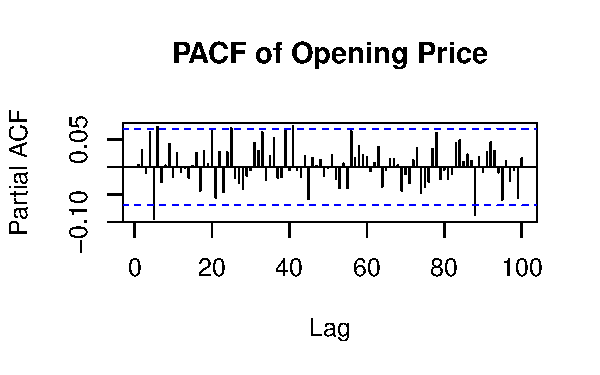
\includegraphics{binary-forex-trading-Q1_files/figure-latex/acf-pacf-1}
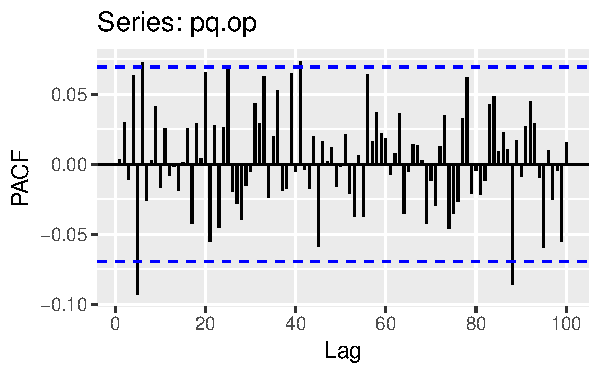
\includegraphics{binary-forex-trading-Q1_files/figure-latex/acf-pacf-2}
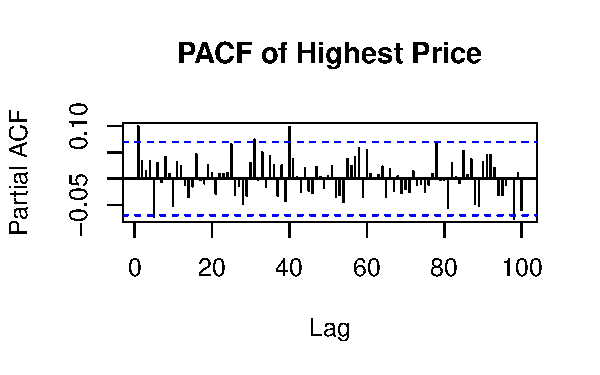
\includegraphics{binary-forex-trading-Q1_files/figure-latex/acf-pacf-3}
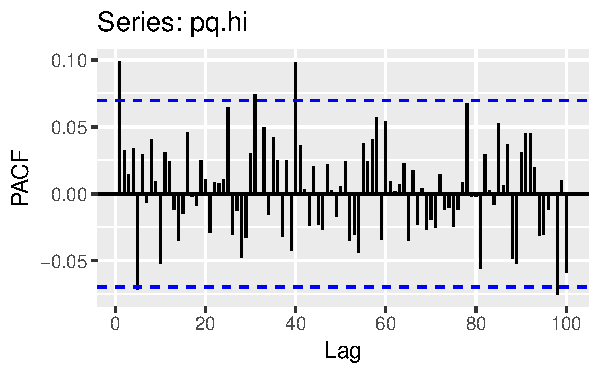
\includegraphics{binary-forex-trading-Q1_files/figure-latex/acf-pacf-4}
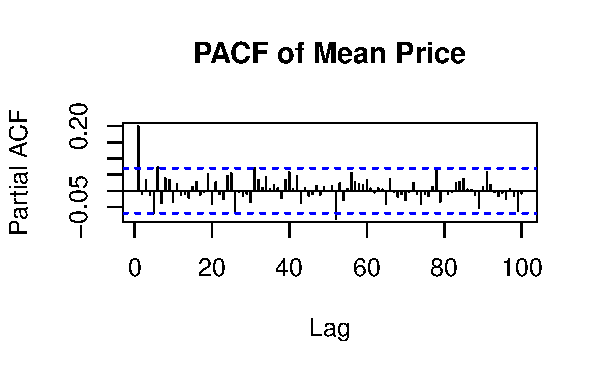
\includegraphics{binary-forex-trading-Q1_files/figure-latex/acf-pacf-5}
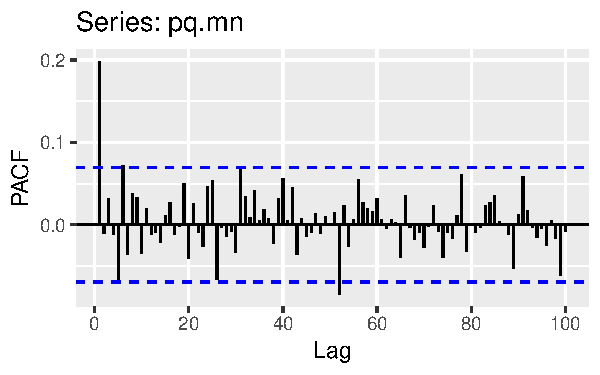
\includegraphics{binary-forex-trading-Q1_files/figure-latex/acf-pacf-6}
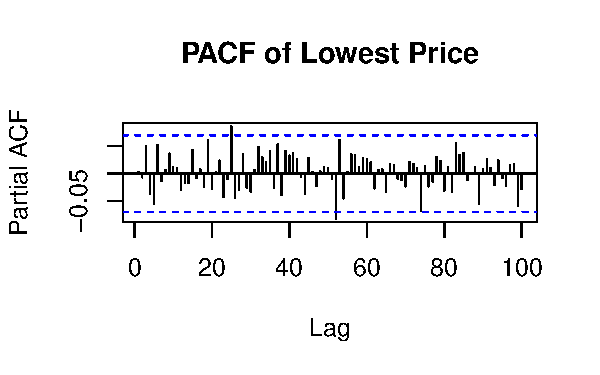
\includegraphics{binary-forex-trading-Q1_files/figure-latex/acf-pacf-7}
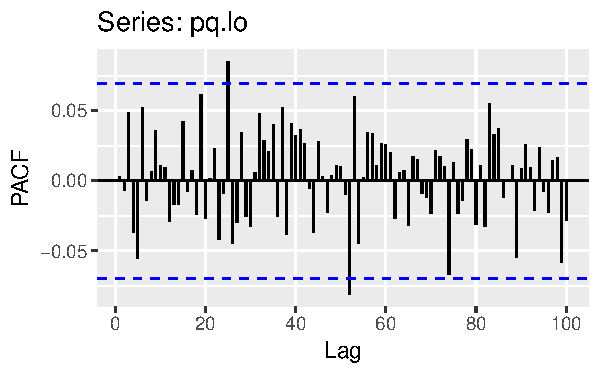
\includegraphics{binary-forex-trading-Q1_files/figure-latex/acf-pacf-8}
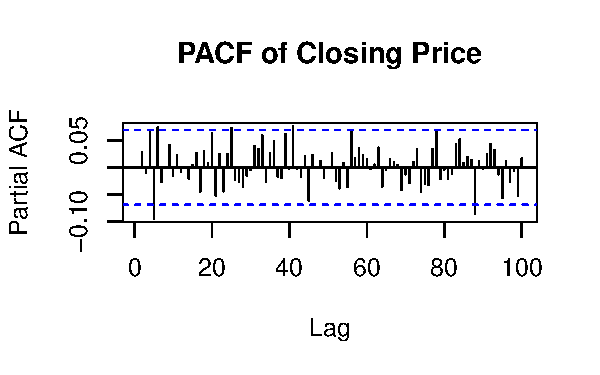
\includegraphics{binary-forex-trading-Q1_files/figure-latex/acf-pacf-9}
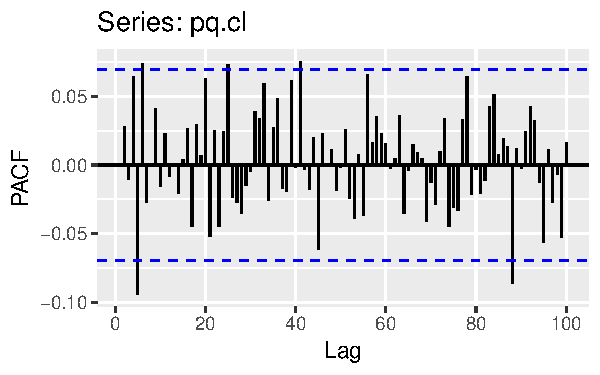
\includegraphics{binary-forex-trading-Q1_files/figure-latex/acf-pacf-10}
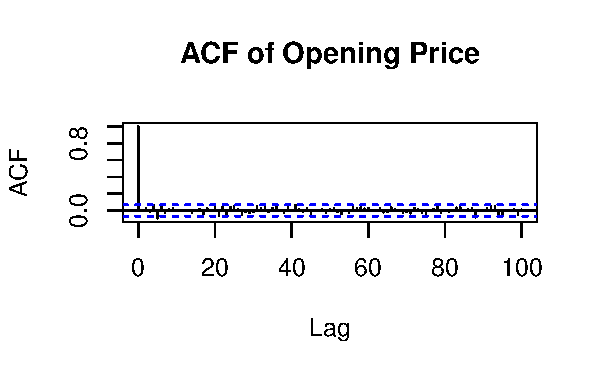
\includegraphics{binary-forex-trading-Q1_files/figure-latex/acf-pacf-11}
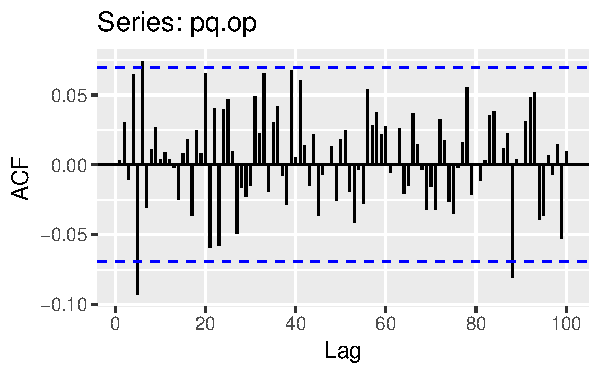
\includegraphics{binary-forex-trading-Q1_files/figure-latex/acf-pacf-12}
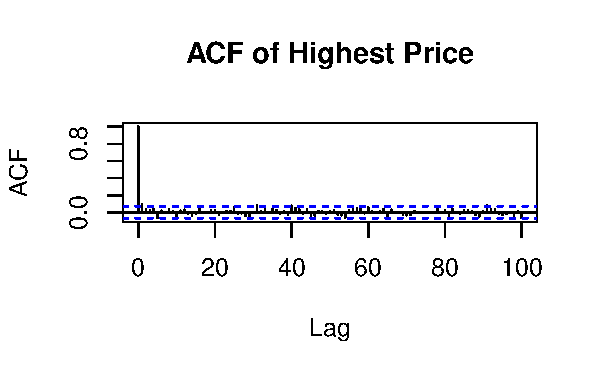
\includegraphics{binary-forex-trading-Q1_files/figure-latex/acf-pacf-13}
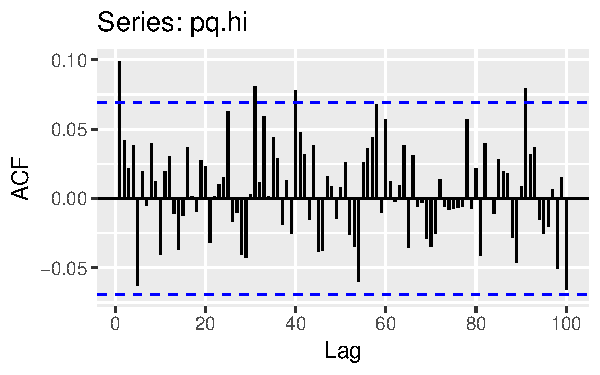
\includegraphics{binary-forex-trading-Q1_files/figure-latex/acf-pacf-14}
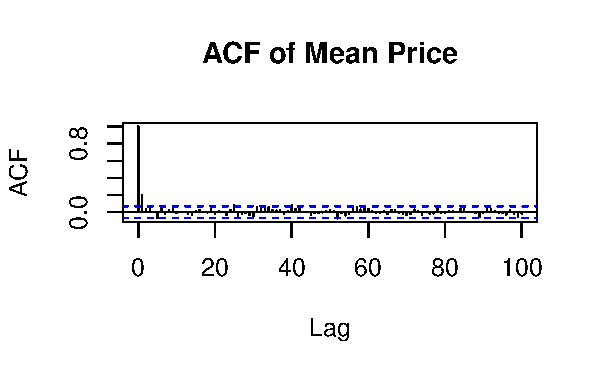
\includegraphics{binary-forex-trading-Q1_files/figure-latex/acf-pacf-15}
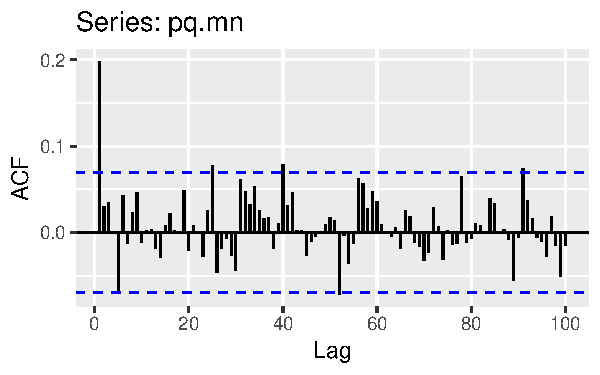
\includegraphics{binary-forex-trading-Q1_files/figure-latex/acf-pacf-16}
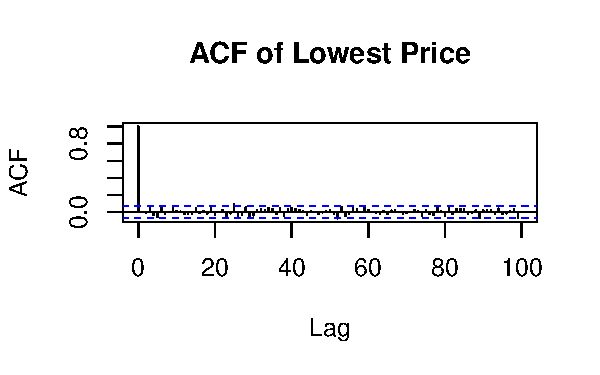
\includegraphics{binary-forex-trading-Q1_files/figure-latex/acf-pacf-17}
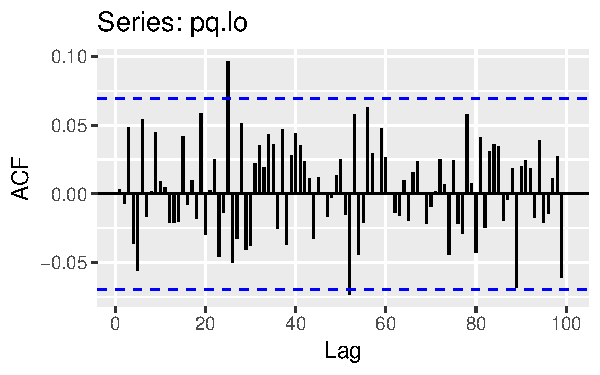
\includegraphics{binary-forex-trading-Q1_files/figure-latex/acf-pacf-18}
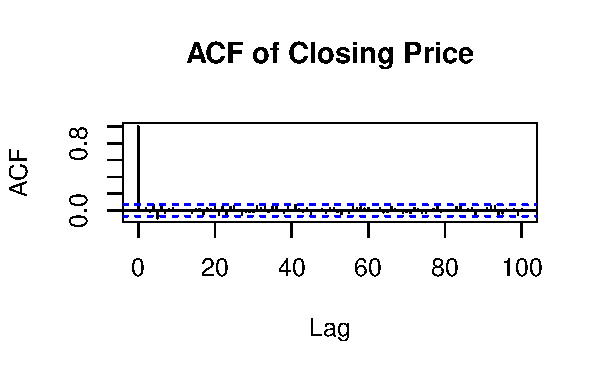
\includegraphics{binary-forex-trading-Q1_files/figure-latex/acf-pacf-19}
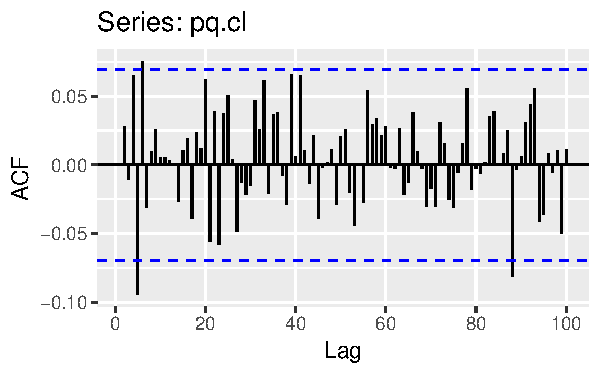
\includegraphics{binary-forex-trading-Q1_files/figure-latex/acf-pacf-20}

Here I use a function to find the optimal value of \texttt{p} and
\texttt{q} from \texttt{armaOrder(0,0)} to \texttt{armaOrder(5,5)} by
refer to
\href{http://blog.csdn.net/u012543538/article/details/38663715}{{R-ARMA(p,q)如何选找最小AIC的p,q值}}.

However, due to optimal \texttt{r} and \texttt{s} for Garch model will
consume alot of time to test the optimal \texttt{garchOrder(r,s)} here I
skip it and just using default \texttt{garchOrder(1,1)}.

\begin{itemize}
\tightlist
\item
  An ARMA(p,q) model specifies the conditional mean of the process
\item
  The GARCH(r,s) model specifies the conditional variance of the process
\end{itemize}

Kindly refer to
\href{https://stats.stackexchange.com/questions/41509/what-is-the-difference-between-garch-and-arma}{{What
is the difference between GARCH and ARMA?}} for more information.

\begin{Shaded}
\begin{Highlighting}[]
\NormalTok{pq.op <-}\StringTok{ }\KeywordTok{suppressWarnings}\NormalTok{(}\KeywordTok{armaSearch}\NormalTok{(}\KeywordTok{Op}\NormalTok{(mbase)))}
\end{Highlighting}
\end{Shaded}

\begin{verbatim}
## method = 'CSS-ML', the min AIC = 1623.45338140965, p = 4, q = 4
\end{verbatim}

\begin{Shaded}
\begin{Highlighting}[]
\NormalTok{pq.hi <-}\StringTok{ }\KeywordTok{suppressWarnings}\NormalTok{(}\KeywordTok{armaSearch}\NormalTok{(}\KeywordTok{Hi}\NormalTok{(mbase)))}
\end{Highlighting}
\end{Shaded}

\begin{verbatim}
## method = 'CSS-ML', the min AIC = 1490.07263872323, p = 4, q = 3
\end{verbatim}

\begin{Shaded}
\begin{Highlighting}[]
\NormalTok{USDJPY.Mean =}\StringTok{ }\NormalTok{(}\KeywordTok{Hi}\NormalTok{(mbase) }\OperatorTok{+}\StringTok{ }\KeywordTok{Lo}\NormalTok{(mbase))}\OperatorTok{/}\DecValTok{2}
\KeywordTok{names}\NormalTok{(USDJPY.Mean) <-}\StringTok{ "USDJPY.Mean"}
\NormalTok{pq.mn <-}\StringTok{ }\KeywordTok{suppressWarnings}\NormalTok{(}\KeywordTok{armaSearch}\NormalTok{(USDJPY.Mean))  }\CommentTok{#force to choose 'ML' since 'CSS-ML' error.}
\end{Highlighting}
\end{Shaded}

\begin{verbatim}
## method = 'CSS-ML', the min AIC = 1369.50193310379, p = 3, q = 2
\end{verbatim}

\begin{Shaded}
\begin{Highlighting}[]
\NormalTok{pq.lo <-}\StringTok{ }\KeywordTok{suppressWarnings}\NormalTok{(}\KeywordTok{armaSearch}\NormalTok{(}\KeywordTok{Lo}\NormalTok{(mbase)))  }\CommentTok{#force to choose 'ML' since 'CSS-ML' error.}
\end{Highlighting}
\end{Shaded}

\begin{verbatim}
## method = 'CSS-ML', the min AIC = 1710.3744852797, p = 2, q = 2
\end{verbatim}

\begin{Shaded}
\begin{Highlighting}[]
\NormalTok{pq.cl <-}\StringTok{ }\KeywordTok{suppressWarnings}\NormalTok{(}\KeywordTok{armaSearch}\NormalTok{(}\KeywordTok{Cl}\NormalTok{(mbase)))}
\end{Highlighting}
\end{Shaded}

\begin{verbatim}
## method = 'CSS-ML', the min AIC = 1634.7817779015, p = 3, q = 3
\end{verbatim}

\begin{Shaded}
\begin{Highlighting}[]
\NormalTok{## From below comparison, we know that the}
\NormalTok{## 'CSS-ML' is better than 'ML'.}
\CommentTok{#'@ > suppressWarnings(armaSearch(Cl(mbase)))}
\CommentTok{# the min AIC = 1635.718 , p = 2 , q = 4 p q}
\CommentTok{# AIC 1 0 0 1641.616 2 0 1 1643.616 3 0 2}
\CommentTok{# 1645.062 4 0 3 1647.036 5 0 4 1645.792 6 0 5}
\CommentTok{# 1639.704 7 1 0 1643.616 8 1 1 1645.616 9 1 2}
\CommentTok{# 1640.169 10 1 3 1640.896 11 1 4 1636.914 12}
\CommentTok{# 1 5 1636.216 13 2 0 1644.991 14 2 1 1640.297}
\CommentTok{# 15 2 2 1642.826 16 2 3 1644.150 17 2 4}
\CommentTok{# 1635.718 18 2 5 1637.614 19 3 0 1646.901 20}
\CommentTok{# 3 1 1641.620 21 3 2 1643.541 22 3 3 1646.957}
\CommentTok{# 23 3 4 1636.964 24 3 5 1639.715 25 4 0}
\CommentTok{# 1645.485 26 4 1 1639.150 27 4 2 1635.929 28}
\CommentTok{# 4 3 1636.975 29 4 4 1638.584 30 4 5 1640.505}
\CommentTok{# 31 5 0 1640.214 32 5 1 1638.289 33 5 2}
\CommentTok{# 1637.855 34 5 3 1639.926 35 5 4 1638.875 36}
\CommentTok{# 5 5 1641.102}
\CommentTok{#'@ > suppressWarnings(armaSearch(Cl(mbase), .method = 'CSS-ML'))}
\CommentTok{# the min AIC = 1634.782 , p = 3 , q = 3 p q}
\CommentTok{# AIC 1 0 0 1641.616 2 0 1 1643.616 3 0 2}
\CommentTok{# 1645.062 4 0 3 1647.036 5 0 4 1645.792 6 0 5}
\CommentTok{# 1639.704 7 1 0 1643.616 8 1 1 1645.616 9 1 2}
\CommentTok{# 1640.168 10 1 3 1640.896 11 1 4 1636.914 12}
\CommentTok{# 1 5 1636.216 13 2 0 1644.991 14 2 1 1640.297}
\CommentTok{# 15 2 2 1642.734 16 2 3 1643.207 17 2 4}
\CommentTok{# 1635.717 18 2 5 1636.222 19 3 0 1646.901 20}
\CommentTok{# 3 1 1641.620 21 3 2 1644.290 22 3 3 1634.782}
\CommentTok{# 23 3 4 1636.240 24 3 5 1638.113 25 4 0}
\CommentTok{# 1645.485 26 4 1 1639.150 27 4 2 1635.929 28}
\CommentTok{# 4 3 1636.975 29 4 4 1638.584 30 4 5 1640.505}
\CommentTok{# 31 5 0 1640.214 32 5 1 1638.289 33 5 2}
\CommentTok{# 1637.855 34 5 3 1639.926 35 5 4 1636.145 36}
\CommentTok{# 5 5 1641.102}

\CommentTok{#'@ > suppressWarnings(armaSearch(Mn(USDJPY.Mean)))}
\CommentTok{# the min AIC = 1369.503 , p = 3 , q = 2 p q}
\CommentTok{# AIC 1 0 0 1408.854 2 0 1 1379.128 3 0 2}
\CommentTok{# 1380.864 4 0 3 1382.213 5 0 4 1383.223 6 0 5}
\CommentTok{# 1377.906 7 1 0 1378.869 8 1 1 1380.755 9 1 2}
\CommentTok{# 1382.479 10 1 3 1384.072 11 1 4 1379.514 12}
\CommentTok{# 1 5 1378.089 13 2 0 1380.792 14 2 1 1382.634}
\CommentTok{# 15 2 2 1384.310 16 2 3 1384.559 17 2 4}
\CommentTok{# 1375.647 18 2 5 1377.609 19 3 0 1381.965 20}
\CommentTok{# 3 1 1383.946 21 3 2 1369.503 22 3 3 1376.475}
\CommentTok{# 23 3 4 1377.613 24 3 5 1379.641 25 4 0}
\CommentTok{# 1383.859 26 4 1 1385.411 27 4 2 1375.856 28}
\CommentTok{# 4 3 1373.091 29 4 4 1378.873 30 4 5 1380.859}
\CommentTok{# 31 5 0 1382.015 32 5 1 1379.627 33 5 2}
\CommentTok{# 1377.687 34 5 3 1379.462 35 5 4 1380.859 36}
\CommentTok{# 5 5 1382.397}
\CommentTok{#'@ > suppressWarnings(armaSearch(Mn(USDJPY.Mean), .method = 'CSS-ML'))}
\CommentTok{# Show Traceback Rerun with Debug Error in}
\CommentTok{# arima(data, order = c(p, 1, q), method =}
\CommentTok{# .method) : non-stationary AR part from CSS}
\CommentTok{#'@ > suppressWarnings(armaSearch(Mn(USDJPY.Mean), .method = 'CSS'))}
\CommentTok{# the min AIC = , p = , q = p q AIC 1 0 0 NA 2}
\CommentTok{# 0 1 NA 3 0 2 NA 4 0 3 NA 5 0 4 NA 6 0 5 NA 7}
\CommentTok{# 1 0 NA 8 1 1 NA 9 1 2 NA 10 1 3 NA 11 1 4 NA}
\CommentTok{# 12 1 5 NA 13 2 0 NA 14 2 1 NA 15 2 2 NA 16 2}
\CommentTok{# 3 NA 17 2 4 NA 18 2 5 NA 19 3 0 NA 20 3 1 NA}
\CommentTok{# 21 3 2 NA 22 3 3 NA 23 3 4 NA 24 3 5 NA 25 4}
\CommentTok{# 0 NA 26 4 1 NA 27 4 2 NA 28 4 3 NA 29 4 4 NA}
\CommentTok{# 30 4 5 NA 31 5 0 NA 32 5 1 NA 33 5 2 NA 34 5}
\CommentTok{# 3 NA 35 5 4 NA 36 5 5 NA}


\CommentTok{#'@ > pq.op <- suppressWarnings(armaSearch(Op(mbase)))}
\CommentTok{# the min AIC = 1623.453 , p = 4 , q = 4}
\CommentTok{#'@ > pq.hi <- suppressWarnings(armaSearch(Hi(mbase)))}
\CommentTok{# the min AIC = 1490.073 , p = 4 , q = 3}
\CommentTok{#'@ > USDJPY.Mean = (Hi(mbase) + Lo(mbase)) / 2}
\CommentTok{#'@ > names(USDJPY.Mean) <- 'USDJPY.Mean'}
\CommentTok{#'@ > pq.mn <- suppressWarnings(armaSearch(USDJPY.Mean))}
\CommentTok{# the min AIC = 1369.503 , p = 3 , q = 2}
\CommentTok{#'@ > pq.lo <- suppressWarnings(armaSearch(Lo(mbase)))}
\CommentTok{# the min AIC = 1711.913 , p = 3 , q = 2}
\CommentTok{#'@ > pq.cl <- suppressWarnings(armaSearch(Cl(mbase)))}
\CommentTok{# the min AIC = 1634.782 , p = 3 , q = 3}
\end{Highlighting}
\end{Shaded}

\begin{Shaded}
\begin{Highlighting}[]
\NormalTok{dstGarch <-}\StringTok{ }\KeywordTok{readRDS}\NormalTok{(}\StringTok{"./data/dstGarch.rds"}\NormalTok{)}
\NormalTok{dst.m <-}\StringTok{ }\KeywordTok{ldply}\NormalTok{(dstGarch, }\ControlFlowTok{function}\NormalTok{(x) x }\OperatorTok\StringTok{ }\NormalTok{dplyr}\OperatorTok{::}\KeywordTok{select}\NormalTok{(BR, }
\NormalTok{    Profit, Bal, RR) }\OperatorTok\StringTok{ }\KeywordTok{tail}\NormalTok{(}\DecValTok{1}\NormalTok{)) }\OperatorTok\StringTok{ }\KeywordTok{mutate}\NormalTok{(}\DataTypeTok{BR =} \DecValTok{1000}\NormalTok{, }
    \DataTypeTok{Profit =}\NormalTok{ Bal }\OperatorTok{-}\StringTok{ }\NormalTok{BR, }\DataTypeTok{RR =}\NormalTok{ Bal}\OperatorTok{/}\NormalTok{BR)}
\CommentTok{# .id BR Profit Bal RR 1 norm 1000 182.7446}
\CommentTok{# 1182.745 1.182745 2 snorm 1000 202.8955}
\CommentTok{# 1202.895 1.202895 3 std 1000 155.7099}
\CommentTok{# 1155.710 1.155710 4 sstd 1000 143.0274}
\CommentTok{# 1143.027 1.143027 5 ged 1000 135.8819}
\CommentTok{# 1135.882 1.135882 6 sged 1000 143.1829}
\CommentTok{# 1143.183 1.143183 7 nig 1000 163.9009}
\CommentTok{# 1163.901 1.163901 8 ghyp 1000 137.0740}
\CommentTok{# 1137.074 1.137074 9 jsu 1000 178.7324}
\CommentTok{# 1178.732 1.178732}

\NormalTok{dst.m }\OperatorTok\StringTok{ }\KeywordTok{kable}\NormalTok{(}\DataTypeTok{width =} \StringTok{"auto"}\NormalTok{)}
\end{Highlighting}
\end{Shaded}

\begin{longtable}[]{@{}lrrrr@{}}
\toprule
.id & BR & Profit & Bal & RR\tabularnewline
\midrule
\endhead
norm & 1000 & 182.7446 & 1182.745 & 1.182745\tabularnewline
snorm & 1000 & 202.8955 & 1202.895 & 1.202895\tabularnewline
std & 1000 & 155.7099 & 1155.710 & 1.155710\tabularnewline
sstd & 1000 & 143.0274 & 1143.027 & 1.143027\tabularnewline
ged & 1000 & 135.8819 & 1135.882 & 1.135882\tabularnewline
sged & 1000 & 143.1829 & 1143.183 & 1.143183\tabularnewline
nig & 1000 & 163.9009 & 1163.901 & 1.163901\tabularnewline
ghyp & 1000 & 137.0740 & 1137.074 & 1.137074\tabularnewline
jsu & 1000 & 178.7324 & 1178.732 & 1.178732\tabularnewline
\bottomrule
\end{longtable}

From above comparison of distribution used, we know that \texttt{snorm}
distribution generates most return. Now we know the best \texttt{p} and
\texttt{q}, solver using \texttt{hybrid}, and best fitted distribution.
Now we try to compare the Garch models.

\begin{Shaded}
\begin{Highlighting}[]
\NormalTok{## ---------- eval = FALSE -------------------}
\NormalTok{## http://www.unstarched.net/2014/01/02/the-realized-garch-model/}
\NormalTok{## https://eranraviv.com/volatility-forecast-evaluation-in-r/}
\NormalTok{## https://eranraviv.com/univariate-volatility-forecast-evaluation/}

\NormalTok{garch.m <-}\StringTok{ }\KeywordTok{suppressAll}\NormalTok{(}\KeywordTok{llply}\NormalTok{(.variance.model.par[}\OperatorTok{-}\DecValTok{2}\NormalTok{], }
    \ControlFlowTok{function}\NormalTok{(vm) \{}
\NormalTok{        z =}\StringTok{ }\KeywordTok{simStakesGarch}\NormalTok{(mbase, }\DataTypeTok{.solver =}\NormalTok{ .solver.par[}\DecValTok{1}\NormalTok{], }
            \DataTypeTok{.prCat =}\NormalTok{ pp[[}\DecValTok{19}\NormalTok{]][}\DecValTok{1}\NormalTok{], }\DataTypeTok{.prCat.method =} \StringTok{"CSS-ML"}\NormalTok{, }
            \DataTypeTok{.baseDate =} \KeywordTok{ymd}\NormalTok{(}\StringTok{"2015-01-01"}\NormalTok{), }\DataTypeTok{.parallel =} \OtherTok{FALSE}\NormalTok{, }
            \DataTypeTok{.progress =} \StringTok{"text"}\NormalTok{, }\DataTypeTok{.setPrice =}\NormalTok{ pp[[}\DecValTok{19}\NormalTok{]][}\DecValTok{2}\NormalTok{], }
            \DataTypeTok{.setPrice.method =} \StringTok{"CSS-ML"}\NormalTok{, }\DataTypeTok{.initialFundSize =} \DecValTok{1000}\NormalTok{, }
            \DataTypeTok{.fundLeverageLog =} \OtherTok{FALSE}\NormalTok{, }\DataTypeTok{.filterBets =} \OtherTok{FALSE}\NormalTok{, }
            \DataTypeTok{.variance.model =} \KeywordTok{list}\NormalTok{(}\DataTypeTok{model =}\NormalTok{ vm, }
                \DataTypeTok{garchOrder =} \KeywordTok{c}\NormalTok{(}\DecValTok{1}\NormalTok{, }\DecValTok{1}\NormalTok{), }\DataTypeTok{submodel =} \OtherTok{NULL}\NormalTok{, }
                \DataTypeTok{external.regressors =} \OtherTok{NULL}\NormalTok{, }\DataTypeTok{variance.targeting =} \OtherTok{FALSE}\NormalTok{), }
            \DataTypeTok{.mean.model =} \KeywordTok{list}\NormalTok{(}\DataTypeTok{armaOrder =} \KeywordTok{c}\NormalTok{(}\DecValTok{1}\NormalTok{, }
                \DecValTok{1}\NormalTok{), }\DataTypeTok{include.mean =} \OtherTok{TRUE}\NormalTok{, }\DataTypeTok{archm =} \OtherTok{FALSE}\NormalTok{, }
                \DataTypeTok{archpow =} \DecValTok{1}\NormalTok{, }\DataTypeTok{arfima =} \OtherTok{FALSE}\NormalTok{, }\DataTypeTok{external.regressors =} \OtherTok{NULL}\NormalTok{, }
                \DataTypeTok{archex =} \OtherTok{FALSE}\NormalTok{), }\DataTypeTok{.dist.model =}\NormalTok{ .dist.model.par[}\DecValTok{2}\NormalTok{], }
            \DataTypeTok{start.pars =} \KeywordTok{list}\NormalTok{(), }\DataTypeTok{fixed.pars =} \KeywordTok{list}\NormalTok{())}
        
\NormalTok{        txt1 <-}\StringTok{ }\KeywordTok{paste0}\NormalTok{(}\StringTok{"saveRDS(z"}\NormalTok{, }\StringTok{", file = './data/"}\NormalTok{, }
\NormalTok{            vm, }\StringTok{"."}\NormalTok{, pp[[}\DecValTok{19}\NormalTok{]][}\DecValTok{1}\NormalTok{], }\StringTok{"."}\NormalTok{, pp[[}\DecValTok{19}\NormalTok{]][}\DecValTok{2}\NormalTok{], }
            \StringTok{"."}\NormalTok{, .dist.model.par[}\DecValTok{2}\NormalTok{], }\StringTok{"."}\NormalTok{, .solver.par[}\DecValTok{1}\NormalTok{], }
            \StringTok{".rds')"}\NormalTok{)}
        \KeywordTok{eval}\NormalTok{(}\KeywordTok{parse}\NormalTok{(}\DataTypeTok{text =}\NormalTok{ txt1))}
        \KeywordTok{cat}\NormalTok{(}\KeywordTok{paste0}\NormalTok{(txt1, }\StringTok{" done!"}\NormalTok{, }\StringTok{"}\CharTok{\textbackslash{}n}\StringTok{"}\NormalTok{))}
        \KeywordTok{rm}\NormalTok{(z)}
\NormalTok{    \}, }\DataTypeTok{.progress =} \StringTok{"text"}\NormalTok{))}
\end{Highlighting}
\end{Shaded}

\begin{Shaded}
\begin{Highlighting}[]
\NormalTok{## load the pre-run and saved models.  Profit}
\NormalTok{## and Loss of Arima models.}

\NormalTok{flsGarchM <-}\StringTok{ }\KeywordTok{dir}\NormalTok{(}\StringTok{"./data"}\NormalTok{, }\DataTypeTok{pattern =} \StringTok{".Mn.Cl.snorm.hybrid"}\NormalTok{)}

\NormalTok{fundList <-}\StringTok{ }\KeywordTok{llply}\NormalTok{(flsGarchM, }\ControlFlowTok{function}\NormalTok{(dt) \{}
\NormalTok{    fl =}\StringTok{ }\KeywordTok{paste0}\NormalTok{(}\StringTok{"./data/"}\NormalTok{, dt)}
    \ControlFlowTok{if}\NormalTok{ (}\KeywordTok{file.size}\NormalTok{(fl) }\OperatorTok{>}\StringTok{ }\DecValTok{100}\NormalTok{) \{}
        \KeywordTok{cbind}\NormalTok{(}\DataTypeTok{Model =} \KeywordTok{str_replace_all}\NormalTok{(dt, }\StringTok{".rds"}\NormalTok{, }
            \StringTok{""}\NormalTok{), }\KeywordTok{readRDS}\NormalTok{(}\DataTypeTok{file =}\NormalTok{ fl)) }\OperatorTok\StringTok{ }\NormalTok{tbl_df}
\NormalTok{    \}}
\NormalTok{\})}

\CommentTok{#'@ names(fundList) <- sapply(fundList, function(x) xts::first(x$Model))}
\KeywordTok{names}\NormalTok{(fundList) <-}\StringTok{ }\NormalTok{flsGarchM }\OperatorTok\StringTok{ }\KeywordTok{str_replace_all}\NormalTok{(}\StringTok{".Mn.Cl.snorm.hybrid.rds"}\NormalTok{, }
    \StringTok{""}\NormalTok{)}
\NormalTok{fundList[}\KeywordTok{sapply}\NormalTok{(fundList, is.null)] <-}\StringTok{ }\OtherTok{NULL}

\NormalTok{## Summary of ROI}
\NormalTok{gm.tbl <-}\StringTok{ }\KeywordTok{ldply}\NormalTok{(fundList, }\ControlFlowTok{function}\NormalTok{(x) \{}
\NormalTok{    x }\OperatorTok\StringTok{ }\KeywordTok{mutate}\NormalTok{(}\DataTypeTok{StartDate =}\NormalTok{ xts}\OperatorTok{::}\KeywordTok{first}\NormalTok{(Date), }
        \DataTypeTok{LatestDate =} \KeywordTok{last}\NormalTok{(Date), }\DataTypeTok{InitFund =}\NormalTok{ xts}\OperatorTok{::}\KeywordTok{first}\NormalTok{(BR), }
        \DataTypeTok{LatestFund =} \KeywordTok{last}\NormalTok{(Bal), }\DataTypeTok{Profit =} \KeywordTok{sum}\NormalTok{(Profit), }
        \DataTypeTok{RR =}\NormalTok{ LatestFund}\OperatorTok{/}\NormalTok{InitFund) }\OperatorTok\StringTok{ }\NormalTok{dplyr}\OperatorTok{::}\KeywordTok{select}\NormalTok{(StartDate, }
\NormalTok{        LatestDate, InitFund, LatestFund, Profit, }
\NormalTok{        RR) }\OperatorTok\StringTok{ }\NormalTok{unique}
\NormalTok{\}) }\OperatorTok\StringTok{ }\NormalTok{tbl_df}
\NormalTok{## The rest omitted due to error.  A tibble: 9}
\NormalTok{## x 7 .id StartDate LatestDate InitFund}
\NormalTok{## LatestFund Profit RR <chr> <date> <date>}
\NormalTok{## <dbl> <dbl> <dbl> <dbl> 1 apARCH 2015-01-02}
\NormalTok{## 2017-01-20 1000 NaN NaN NaN 2 csGARCH}
\NormalTok{## 2015-01-02 2017-01-20 1000 NaN NaN NaN 3}
\NormalTok{## eGARCH 1970-01-02 1971-06-20 1000 1182.745}
\NormalTok{## 182.7446 1.182745 4 fGARCH.APARCH 2015-01-02}
\NormalTok{## 2017-01-20 1000 NaN NaN NaN 5 fGARCH.GARCH}
\NormalTok{## 2015-01-02 2017-01-20 1000 1177.530 177.5298}
\NormalTok{## 1.177530 6 fGARCH.GJRGARCH 2015-01-02}
\NormalTok{## 2017-01-20 1000 1204.554 204.5541 1.204554 7}
\NormalTok{## gjrGARCH 2015-01-02 2017-01-20 1000 1189.793}
\NormalTok{## 189.7935 1.189793 8 iGARCH 2015-01-02}
\NormalTok{## 2017-01-20 1000 1191.571 191.5711 1.191571 9}
\NormalTok{## sGARCH 2015-01-02 2017-01-20 1000 1196.402}
\NormalTok{## 196.4022 1.196402}

\NormalTok{gm.tbl }\OperatorTok\StringTok{ }\KeywordTok{kable}\NormalTok{(}\DataTypeTok{width =} \StringTok{"auto"}\NormalTok{)}
\end{Highlighting}
\end{Shaded}

\begin{longtable}[]{@{}lllrrrr@{}}
\toprule
.id & StartDate & LatestDate & InitFund & LatestFund & Profit &
RR\tabularnewline
\midrule
\endhead
apARCH & 2015-01-02 & 2017-01-20 & 1000 & NaN & NaN & NaN\tabularnewline
csGARCH & 2015-01-02 & 2017-01-20 & 1000 & NaN & NaN &
NaN\tabularnewline
eGARCH & 1970-01-02 & 1971-06-20 & 1000 & 1182.745 & 182.7446 &
1.182745\tabularnewline
fGARCH.APARCH & 2015-01-02 & 2017-01-20 & 1000 & NaN & NaN &
NaN\tabularnewline
fGARCH.GARCH & 2015-01-02 & 2017-01-20 & 1000 & 1177.530 & 177.5298 &
1.177530\tabularnewline
fGARCH.GJRGARCH & 2015-01-02 & 2017-01-20 & 1000 & 1204.554 & 204.5540 &
1.204554\tabularnewline
gjrGARCH & 2015-01-02 & 2017-01-20 & 1000 & 1189.829 & 189.8295 &
1.189830\tabularnewline
iGARCH & 2015-01-02 & 2017-01-20 & 1000 & 1191.571 & 191.5711 &
1.191571\tabularnewline
sGARCH & 2015-01-02 & 2017-01-20 & 1000 & 1196.402 & 196.4022 &
1.196402\tabularnewline
\bottomrule
\end{longtable}

We know from above table that model \texttt{fGARCH.GJRGARCH} generates
most return. Here I do combine the components/parameters of Garch models
to get the best among them.

\begin{Shaded}
\begin{Highlighting}[]
\NormalTok{## load the pre-run and saved models.  Profit}
\NormalTok{## and Loss of Arima models.}

\NormalTok{flsGarchM <-}\StringTok{ }\KeywordTok{dir}\NormalTok{(}\StringTok{"./data"}\NormalTok{, }\DataTypeTok{pattern =} \StringTok{"^fGARCH.GJRGARCH+.+.snorm.hybrid"}\NormalTok{)}

\NormalTok{fundList <-}\StringTok{ }\KeywordTok{llply}\NormalTok{(flsGarchM, }\ControlFlowTok{function}\NormalTok{(dt) \{}
\NormalTok{    fl =}\StringTok{ }\KeywordTok{paste0}\NormalTok{(}\StringTok{"./data/"}\NormalTok{, dt)}
    \ControlFlowTok{if}\NormalTok{ (}\KeywordTok{file.size}\NormalTok{(fl) }\OperatorTok{>}\StringTok{ }\DecValTok{100}\NormalTok{) \{}
        \KeywordTok{cbind}\NormalTok{(}\DataTypeTok{Model =} \KeywordTok{str_replace_all}\NormalTok{(dt, }\StringTok{".rds"}\NormalTok{, }
            \StringTok{""}\NormalTok{), }\KeywordTok{readRDS}\NormalTok{(}\DataTypeTok{file =}\NormalTok{ fl)) }\OperatorTok\StringTok{ }\NormalTok{tbl_df}
\NormalTok{    \}}
\NormalTok{\})}

\CommentTok{#'@ names(fundList) <- sapply(fundList, function(x) xts::first(x$Model))}
\KeywordTok{names}\NormalTok{(fundList) <-}\StringTok{ }\NormalTok{flsGarchM }\OperatorTok\StringTok{ }\KeywordTok{str_replace_all}\NormalTok{(}\StringTok{".Mn.Cl.snorm.hybrid.rds"}\NormalTok{, }
    \StringTok{""}\NormalTok{)}
\NormalTok{fundList[}\KeywordTok{sapply}\NormalTok{(fundList, is.null)] <-}\StringTok{ }\OtherTok{NULL}

\NormalTok{## Summary of ROI}
\NormalTok{gm.tbl <-}\StringTok{ }\KeywordTok{ldply}\NormalTok{(fundList, }\ControlFlowTok{function}\NormalTok{(x) \{}
\NormalTok{    x }\OperatorTok\StringTok{ }\KeywordTok{mutate}\NormalTok{(}\DataTypeTok{StartDate =}\NormalTok{ xts}\OperatorTok{::}\KeywordTok{first}\NormalTok{(Date), }
        \DataTypeTok{LatestDate =} \KeywordTok{last}\NormalTok{(Date), }\DataTypeTok{InitFund =}\NormalTok{ xts}\OperatorTok{::}\KeywordTok{first}\NormalTok{(BR), }
        \DataTypeTok{LatestFund =} \KeywordTok{last}\NormalTok{(Bal), }\DataTypeTok{Profit =} \KeywordTok{sum}\NormalTok{(Profit), }
        \DataTypeTok{RR =}\NormalTok{ LatestFund}\OperatorTok{/}\NormalTok{InitFund) }\OperatorTok\StringTok{ }\NormalTok{dplyr}\OperatorTok{::}\KeywordTok{select}\NormalTok{(StartDate, }
\NormalTok{        LatestDate, InitFund, LatestFund, Profit, }
\NormalTok{        RR) }\OperatorTok\StringTok{ }\NormalTok{unique}
\NormalTok{\}) }\OperatorTok\StringTok{ }\NormalTok{tbl_df}
\NormalTok{## A tibble: 20 x 7 .id StartDate LatestDate}
\NormalTok{## InitFund LatestFund Profit RR <chr> <date>}
\NormalTok{## <date> <dbl> <dbl> #<dbl> <dbl> 1}
\NormalTok{## gjrGARCH.Cl.Hi.snorm.hybrid.rds 2015-01-02}
\NormalTok{## 2017-01-20 1000 1320.381 320.3809 1.320381 2}
\NormalTok{## gjrGARCH.Cl.Lo.snorm.hybrid.rds 2015-01-02}
\NormalTok{## 2017-01-20 1000 1342.644 342.6443 1.342644 3}
\NormalTok{## gjrGARCH.Cl.Mn.snorm.hybrid.rds 2015-01-02}
\NormalTok{## 2017-01-20 1000 1293.483 293.4827 1.293483 4}
\NormalTok{## gjrGARCH.Cl.Op.snorm.hybrid.rds 2015-01-02}
\NormalTok{## 2017-01-20 1000 1128.494 128.4942 1.128494 5}
\NormalTok{## gjrGARCH.Hi.Cl.snorm.hybrid.rds 2015-01-02}
\NormalTok{## 2017-01-20 1000 NaN NaN NaN 6}
\NormalTok{## gjrGARCH.Hi.Lo.snorm.hybrid.rds 2015-01-02}
\NormalTok{## 2017-01-20 1000 1684.614 684.6141 1.684614 7}
\NormalTok{## gjrGARCH.Hi.Mn.snorm.hybrid.rds 2015-01-02}
\NormalTok{## 2017-01-20 1000 1398.689 398.6890 1.398689 8}
\NormalTok{## gjrGARCH.Hi.Op.snorm.hybrid.rds 2015-01-02}
\NormalTok{## 2017-01-20 1000 NaN NaN NaN 9}
\NormalTok{## gjrGARCH.Lo.Cl.snorm.hybrid.rds 2015-01-02}
\NormalTok{## 2017-01-20 1000 NaN NaN NaN 10}
\NormalTok{## gjrGARCH.Lo.Hi.snorm.hybrid.rds 2015-01-02}
\NormalTok{## 2017-01-20 1000 1730.533 730.5325 1.730533}
\NormalTok{## 11 gjrGARCH.Lo.Mn.snorm.hybrid.rds}
\NormalTok{## 2015-01-02 2017-01-20 1000 1394.744 394.7443}
\NormalTok{## 1.394744 12 gjrGARCH.Lo.Op.snorm.hybrid.rds}
\NormalTok{## 2015-01-02 2017-01-20 1000 NaN NaN NaN 13}
\NormalTok{## gjrGARCH 2015-01-02 2017-01-20 1000 1189.829}
\NormalTok{## 189.8295 1.189829 14}
\NormalTok{## gjrGARCH.Mn.Hi.snorm.hybrid.rds 2015-01-02}
\NormalTok{## 2017-01-20 1000 1280.016 280.0165 1.280016}
\NormalTok{## 15 gjrGARCH.Mn.Lo.snorm.hybrid.rds}
\NormalTok{## 2015-01-02 2017-01-20 1000 1213.700 213.6997}
\NormalTok{## 1.213700 16 gjrGARCH.Mn.Op.snorm.hybrid.rds}
\NormalTok{## 2015-01-02 2017-01-20 1000 1177.741 177.7413}
\NormalTok{## 1.177741 17 gjrGARCH.Op.Cl.snorm.hybrid.rds}
\NormalTok{## 2015-01-02 2017-01-20 1000 1180.072 180.0717}
\NormalTok{## 1.180072 18 gjrGARCH.Op.Hi.snorm.hybrid.rds}
\NormalTok{## 2015-01-02 2017-01-20 1000 NaN NaN NaN 19}
\NormalTok{## gjrGARCH.Op.Lo.snorm.hybrid.rds 2015-01-02}
\NormalTok{## 2017-01-20 1000 1302.291 302.2906 1.302291}
\NormalTok{## 20 gjrGARCH.Op.Mn.snorm.hybrid.rds}
\NormalTok{## 2015-01-02 2017-01-20 1000 1324.539 324.5393}
\NormalTok{## 1.324539}

\NormalTok{gm.tbl }\OperatorTok\StringTok{ }\KeywordTok{kable}\NormalTok{(}\DataTypeTok{width =} \StringTok{"auto"}\NormalTok{)}
\end{Highlighting}
\end{Shaded}

\begin{longtable}[]{@{}lllrrrr@{}}
\toprule
.id & StartDate & LatestDate & InitFund & LatestFund & Profit &
RR\tabularnewline
\midrule
\endhead
fGARCH.GJRGARCH.Cl.Lo.snorm.hybrid.rds & 2015-01-02 & 2017-01-20 & 1000
& 1277.813 & 277.8132 & 1.277813\tabularnewline
fGARCH.GJRGARCH.Cl.Mn.snorm.hybrid.rds & 2015-01-02 & 2017-01-20 & 1000
& 1297.879 & 297.8787 & 1.297879\tabularnewline
fGARCH.GJRGARCH.Lo.Cl.snorm.hybrid.rds & 2015-01-02 & 2017-01-20 & 1000
& 1467.495 & 467.4955 & 1.467496\tabularnewline
fGARCH.GJRGARCH.Lo.Mn.snorm.hybrid.rds & 2015-01-02 & 2017-01-20 & 1000
& 1369.321 & 369.3214 & 1.369321\tabularnewline
fGARCH.GJRGARCH.Lo.Op.snorm.hybrid.rds & 2015-01-02 & 2017-01-20 & 1000
& 1474.156 & 474.1564 & 1.474156\tabularnewline
fGARCH.GJRGARCH & 2015-01-02 & 2017-01-20 & 1000 & 1204.554 & 204.5540 &
1.204554\tabularnewline
fGARCH.GJRGARCH.Mn.Lo.snorm.hybrid.rds & 2015-01-02 & 2017-01-20 & 1000
& 1288.168 & 288.1677 & 1.288168\tabularnewline
fGARCH.GJRGARCH.Mn.Op.snorm.hybrid.rds & 2015-01-02 & 2017-01-20 & 1000
& 1151.503 & 151.5030 & 1.151503\tabularnewline
fGARCH.GJRGARCH.Op.Cl.snorm.hybrid.rds & 2015-01-02 & 2017-01-20 & 1000
& 1168.411 & 168.4106 & 1.168411\tabularnewline
fGARCH.GJRGARCH.Op.Lo.snorm.hybrid.rds & 2015-01-02 & 2017-01-20 & 1000
& 1281.735 & 281.7350 & 1.281735\tabularnewline
fGARCH.GJRGARCH.Op.Mn.snorm.hybrid.rds & 2015-01-02 & 2017-01-20 & 1000
& 1267.692 & 267.6919 & 1.267692\tabularnewline
\bottomrule
\end{longtable}

From above table, we concludes below ROI.

\begin{verbatim}
# 6 gjrGARCH.Hi.Lo.snorm.hybrid.rds 2015-01-02 2017-01-20     1000   1684.614 684.6141 1.684614
#10 gjrGARCH.Lo.Hi.snorm.hybrid.rds 2015-01-02 2017-01-20     1000   1730.533 730.5325 1.730533
\end{verbatim}

\textbf{Volatility Staking}

\begin{Shaded}
\begin{Highlighting}[]
\NormalTok{## load the pre-run and saved models.  Profit}
\NormalTok{## and Loss of Arima models.}

\NormalTok{flsGarchM <-}\StringTok{ }\KeywordTok{dir}\NormalTok{(}\StringTok{"./data"}\NormalTok{, }\DataTypeTok{pattern =} \StringTok{".snorm.hybrid"}\NormalTok{)}

\NormalTok{fundList <-}\StringTok{ }\KeywordTok{llply}\NormalTok{(flsGarchM, }\ControlFlowTok{function}\NormalTok{(dt) \{}
\NormalTok{    fl =}\StringTok{ }\KeywordTok{paste0}\NormalTok{(}\StringTok{"./data/"}\NormalTok{, dt)}
    \ControlFlowTok{if}\NormalTok{ (}\KeywordTok{file.size}\NormalTok{(fl) }\OperatorTok{>}\StringTok{ }\DecValTok{100}\NormalTok{) \{}
        \KeywordTok{cbind}\NormalTok{(}\DataTypeTok{Model =} \KeywordTok{str_replace_all}\NormalTok{(dt, }\StringTok{".rds"}\NormalTok{, }
            \StringTok{""}\NormalTok{), }\KeywordTok{readRDS}\NormalTok{(}\DataTypeTok{file =}\NormalTok{ fl)) }\OperatorTok\StringTok{ }\NormalTok{tbl_df}
\NormalTok{    \}}
\NormalTok{\})}

\CommentTok{#'@ names(fundList) <- sapply(fundList, function(x) xts::first(x$Model))}
\KeywordTok{names}\NormalTok{(fundList) <-}\StringTok{ }\NormalTok{flsGarchM }\OperatorTok\StringTok{ }\KeywordTok{str_replace_all}\NormalTok{(}\StringTok{".snorm.hybrid.rds"}\NormalTok{, }
    \StringTok{""}\NormalTok{)}
\NormalTok{fundList[}\KeywordTok{sapply}\NormalTok{(fundList, is.null)] <-}\StringTok{ }\OtherTok{NULL}

\NormalTok{## Summary of ROI}
\NormalTok{gm.tbl <-}\StringTok{ }\KeywordTok{ldply}\NormalTok{(fundList, }\ControlFlowTok{function}\NormalTok{(x) \{}
\NormalTok{    x }\OperatorTok\StringTok{ }\KeywordTok{mutate}\NormalTok{(}\DataTypeTok{StartDate =}\NormalTok{ xts}\OperatorTok{::}\KeywordTok{first}\NormalTok{(Date), }
        \DataTypeTok{LatestDate =} \KeywordTok{last}\NormalTok{(Date), }\DataTypeTok{InitFund =}\NormalTok{ xts}\OperatorTok{::}\KeywordTok{first}\NormalTok{(BR), }
        \DataTypeTok{LatestFund =} \KeywordTok{last}\NormalTok{(Bal), }\DataTypeTok{Profit =} \KeywordTok{sum}\NormalTok{(Profit), }
        \DataTypeTok{RR =}\NormalTok{ LatestFund}\OperatorTok{/}\NormalTok{InitFund) }\OperatorTok\StringTok{ }\NormalTok{dplyr}\OperatorTok{::}\KeywordTok{select}\NormalTok{(StartDate, }
\NormalTok{        LatestDate, InitFund, LatestFund, Profit, }
\NormalTok{        RR) }\OperatorTok\StringTok{ }\NormalTok{unique}
\NormalTok{\}) }\OperatorTok\StringTok{ }\NormalTok{tbl_df}
\end{Highlighting}
\end{Shaded}

\begin{Shaded}
\begin{Highlighting}[]
\NormalTok{## Focast the variance and convert to}
\NormalTok{## probability.}
\NormalTok{varHL <-}\StringTok{ }\NormalTok{fundList[}\KeywordTok{grep}\NormalTok{(}\StringTok{"Hi.Lo|Lo.Hi"}\NormalTok{, }\KeywordTok{names}\NormalTok{(fundList))]}
\NormalTok{ntm <-}\StringTok{ }\KeywordTok{c}\NormalTok{(}\KeywordTok{names}\NormalTok{((varHL)[}\KeywordTok{names}\NormalTok{(varHL) }\OperatorTok\StringTok{ }\KeywordTok{c}\NormalTok{(}\StringTok{"Date"}\NormalTok{, }
    \StringTok{"USDJPY.High"}\NormalTok{, }\StringTok{"USDJPY.Low"}\NormalTok{, }\StringTok{"USDJPY.Close"}\NormalTok{)]), }
    \KeywordTok{names}\NormalTok{((varHL)[}\OperatorTok{!}\KeywordTok{names}\NormalTok{(varHL) }\OperatorTok\StringTok{ }\KeywordTok{c}\NormalTok{(}\StringTok{"Date"}\NormalTok{, }
        \StringTok{"USDJPY.High"}\NormalTok{, }\StringTok{"USDJPY.Low"}\NormalTok{, }\StringTok{"USDJPY.Close"}\NormalTok{)])) }\OperatorTok\StringTok{ }
\StringTok{    }\KeywordTok{str_replace}\NormalTok{(}\StringTok{".Hi.Lo|.Lo.Hi"}\NormalTok{, }\StringTok{""}\NormalTok{) }\OperatorTok\StringTok{ }\NormalTok{unique }\OperatorTok\StringTok{ }
\StringTok{    }\NormalTok{sort}

\NormalTok{varHL1 <-}\StringTok{ }\KeywordTok{suppressMessages}\NormalTok{(}\KeywordTok{llply}\NormalTok{(varHL, }\ControlFlowTok{function}\NormalTok{(dtx) \{}
\NormalTok{    mm =}\StringTok{ }\KeywordTok{tbl_df}\NormalTok{(dtx) }\OperatorTok\StringTok{ }\NormalTok{dplyr}\OperatorTok{::}\KeywordTok{select}\NormalTok{(Date, USDJPY.High, }
\NormalTok{        USDJPY.Low, USDJPY.Close, Point.Forecast)}
    \KeywordTok{names}\NormalTok{(mm)[}\DecValTok{5}\NormalTok{] =}\StringTok{ }\KeywordTok{as.character}\NormalTok{(dtx}\OperatorTok{$}\NormalTok{Model[}\DecValTok{1}\NormalTok{])}
    \KeywordTok{names}\NormalTok{(mm) =}\StringTok{ }\KeywordTok{str_replace_all}\NormalTok{(}\KeywordTok{names}\NormalTok{(mm), }\StringTok{"Hi.Lo.snorm.hybrid"}\NormalTok{, }
        \StringTok{"High"}\NormalTok{)}
    \KeywordTok{names}\NormalTok{(mm) =}\StringTok{ }\KeywordTok{str_replace_all}\NormalTok{(}\KeywordTok{names}\NormalTok{(mm), }\StringTok{"Lo.Hi.snorm.hybrid"}\NormalTok{, }
        \StringTok{"Low"}\NormalTok{)}
\NormalTok{    mm}
\NormalTok{\}) }\OperatorTok\StringTok{ }\NormalTok{join_all) }\OperatorTok\StringTok{ }\NormalTok{tbl_df}

\NormalTok{varHL2 <-}\StringTok{ }\KeywordTok{suppressMessages}\NormalTok{(}\KeywordTok{llply}\NormalTok{(ntm, }\ControlFlowTok{function}\NormalTok{(nm) \{}
\NormalTok{    mld =}\StringTok{ }\NormalTok{varHL1[}\KeywordTok{grep}\NormalTok{(nm, }\KeywordTok{names}\NormalTok{(varHL1))]}
\NormalTok{    mld[, }\DecValTok{3}\NormalTok{] =}\StringTok{ }\KeywordTok{abs}\NormalTok{(mld[, }\DecValTok{1}\NormalTok{] }\OperatorTok{-}\StringTok{ }\NormalTok{mld[, }\DecValTok{2}\NormalTok{])}
    \KeywordTok{names}\NormalTok{(mld)[}\DecValTok{3}\NormalTok{] =}\StringTok{ }\KeywordTok{paste0}\NormalTok{(nm, }\StringTok{".Rng"}\NormalTok{)}
\NormalTok{    mld =}\StringTok{ }\NormalTok{mld[}\KeywordTok{colSums}\NormalTok{(}\OperatorTok{!}\KeywordTok{is.na}\NormalTok{(mld)) }\OperatorTok{>}\StringTok{ }\DecValTok{0}\NormalTok{]}
    \KeywordTok{data.frame}\NormalTok{(varHL1[}\KeywordTok{c}\NormalTok{(}\StringTok{"Date"}\NormalTok{, }\StringTok{"USDJPY.High"}\NormalTok{, }
        \StringTok{"USDJPY.Low"}\NormalTok{, }\StringTok{"USDJPY.Close"}\NormalTok{)], }\DataTypeTok{USDJPY.Rng =} \KeywordTok{abs}\NormalTok{(varHL1}\OperatorTok{$}\NormalTok{USDJPY.High }\OperatorTok{-}\StringTok{ }
\StringTok{        }\NormalTok{varHL1}\OperatorTok{$}\NormalTok{USDJPY.Low), mld) }\OperatorTok\StringTok{ }\NormalTok{tbl_df}
\NormalTok{\}) }\OperatorTok\StringTok{ }\NormalTok{unique }\OperatorTok\StringTok{ }\NormalTok{join_all }\OperatorTok\StringTok{ }\NormalTok{tbl_df)}
\end{Highlighting}
\end{Shaded}

\begin{Shaded}
\begin{Highlighting}[]
\NormalTok{## Application of MASS::mvrnorm() or}
\NormalTok{## mvtnorm::rmvnorm() ##nope}
\CommentTok{#'@ varHL2 <- xts(varHL2[, -1], as.Date(varHL2$Date))}

\NormalTok{## Betting strategy 1 - Normal range betting}
\NormalTok{varB1 <-}\StringTok{ }\NormalTok{varHL2[, }\KeywordTok{c}\NormalTok{(}\StringTok{"Date"}\NormalTok{, }\KeywordTok{names}\NormalTok{(varHL2)[}\KeywordTok{str_detect}\NormalTok{(}\KeywordTok{names}\NormalTok{(varHL2), }
    \StringTok{".Rng"}\NormalTok{)])]}

\NormalTok{varB1 <-}\StringTok{ }\KeywordTok{suppressMessages}\NormalTok{(}\KeywordTok{llply}\NormalTok{(ntm, }\ControlFlowTok{function}\NormalTok{(nm) \{}
\NormalTok{    dtx =}\StringTok{ }\KeywordTok{bind_cols}\NormalTok{(varB1[}\KeywordTok{c}\NormalTok{(}\StringTok{"USDJPY.Rng"}\NormalTok{)], varB1[}\KeywordTok{grep}\NormalTok{(nm, }
        \KeywordTok{names}\NormalTok{(varB1))]) }\OperatorTok\StringTok{ }\KeywordTok{mutate_if}\NormalTok{(is.numeric, }
        \KeywordTok{funs}\NormalTok{(}\KeywordTok{ifelse}\NormalTok{(USDJPY.Rng }\OperatorTok{>=}\StringTok{ }\NormalTok{., ., }\OperatorTok{-}\DecValTok{100}\NormalTok{)))}
\NormalTok{    dtx2 =}\StringTok{ }\NormalTok{dtx[, }\DecValTok{2}\NormalTok{] }\OperatorTok\StringTok{ }\KeywordTok{mutate_if}\NormalTok{(is.numeric, }
        \KeywordTok{funs}\NormalTok{(}\KeywordTok{ifelse}\NormalTok{(. }\OperatorTok{>=}\StringTok{ }\DecValTok{0}\NormalTok{, }\DecValTok{100}\NormalTok{, }\OperatorTok{-}\DecValTok{100}\NormalTok{)))}
\NormalTok{    dtx3 =}\StringTok{ }\NormalTok{dtx2 }\OperatorTok\StringTok{ }\KeywordTok{mutate_if}\NormalTok{(is.numeric, }\KeywordTok{funs}\NormalTok{(}\KeywordTok{cumsum}\NormalTok{(.) }\OperatorTok{+}\StringTok{ }
\StringTok{        }\DecValTok{1000}\NormalTok{))}
\NormalTok{    dtx4 =}\StringTok{ }\NormalTok{dtx2 }\OperatorTok\StringTok{ }\KeywordTok{mutate_if}\NormalTok{(is.numeric, }\KeywordTok{funs}\NormalTok{(}\KeywordTok{lag}\NormalTok{(}\DecValTok{1000} \OperatorTok{+}\StringTok{ }
\StringTok{        }\KeywordTok{cumsum}\NormalTok{(.))))}
\NormalTok{    dtx4[}\DecValTok{1}\NormalTok{, }\DecValTok{1}\NormalTok{] =}\StringTok{ }\DecValTok{1000}
\NormalTok{    dtx5 =}\StringTok{ }\KeywordTok{bind_cols}\NormalTok{(varB1[}\StringTok{"Date"}\NormalTok{], dtx4, dtx2, }
\NormalTok{        dtx3)}
    \KeywordTok{names}\NormalTok{(dtx5) =}\StringTok{ }\KeywordTok{names}\NormalTok{(dtx5) }\OperatorTok\StringTok{ }\KeywordTok{str_replace_all}\NormalTok{(}\StringTok{"Rng2"}\NormalTok{, }
        \StringTok{"Bal"}\NormalTok{)}
    \KeywordTok{names}\NormalTok{(dtx5) =}\StringTok{ }\KeywordTok{names}\NormalTok{(dtx5) }\OperatorTok\StringTok{ }\KeywordTok{str_replace_all}\NormalTok{(}\StringTok{"Rng1"}\NormalTok{, }
        \StringTok{"PL"}\NormalTok{)}
    \KeywordTok{names}\NormalTok{(dtx5) =}\StringTok{ }\KeywordTok{names}\NormalTok{(dtx5) }\OperatorTok\StringTok{ }\KeywordTok{str_replace_all}\NormalTok{(}\StringTok{"Rng"}\NormalTok{, }
        \StringTok{"BR"}\NormalTok{)}
\NormalTok{    dtx5}
\NormalTok{\}) }\OperatorTok\StringTok{ }\NormalTok{join_all }\OperatorTok\StringTok{ }\NormalTok{tbl_df)}

\NormalTok{## shows the last 6 balance (ROI)}
\KeywordTok{tail}\NormalTok{(}\KeywordTok{data.frame}\NormalTok{(varB1[}\StringTok{"Date"}\NormalTok{], varB1[}\KeywordTok{grep}\NormalTok{(}\StringTok{"Bal"}\NormalTok{, }
    \KeywordTok{names}\NormalTok{(varB1))])) }\OperatorTok\StringTok{ }\KeywordTok{kable}\NormalTok{(}\DataTypeTok{width =} \StringTok{"auto"}\NormalTok{)}
\end{Highlighting}
\end{Shaded}

\begin{longtable}[]{@{}llrrrrr@{}}
\toprule
& Date & csGARCH.Bal & fGARCH.GARCH.Bal & fGARCH.NGARCH.Bal &
gjrGARCH.Bal & iGARCH.Bal\tabularnewline
\midrule
\endhead
530 & 2017-01-13 & -1000 & -200 & -200 & 1000 & -1800\tabularnewline
531 & 2017-01-16 & -1100 & -300 & -300 & 900 & -1900\tabularnewline
532 & 2017-01-17 & -1000 & -200 & -200 & 1000 & -1800\tabularnewline
533 & 2017-01-18 & -1100 & -300 & -300 & 900 & -1900\tabularnewline
534 & 2017-01-19 & -1000 & -200 & -200 & 1000 & -1800\tabularnewline
535 & 2017-01-20 & -1100 & -300 & -300 & 900 & -1900\tabularnewline
\bottomrule
\end{longtable}

\\

\hypertarget{LineChartID54307ed37f2}{}

\subsubsection{2.1.6.3 MCMC vs Bayesian Time
Series}\label{mcmc-vs-bayesian-time-series-4}

\subsubsection{2.1.6.4 MIDAS}\label{midas-4}

\subsection{2.1.7 Conclusion}\label{conclusion}

\section{2.2 Question 2}\label{question-2}

\section{2.3 Question 3}\label{question-3}

\chapter{3. Conclusion}\label{conclusion-1}

\chapter{4. Appendix}\label{appendix}

\section{4.1 Documenting File Creation}\label{documenting-file-creation}

It's useful to record some information about how your file was created.

\begin{itemize}
\tightlist
\item
  File creation date: 2015-07-22
\item
  File latest updated date: 2017-09-14
\item
  R version 3.4.1 (2017-06-30)
\item
  R version (short form): 3.4.1
\item
  \href{https://github.com/rstudio/rmarkdown}{{\textbf{rmarkdown}
  package}} version: 1.6
\item
  \href{https://github.com/rstudio/tufte}{{\textbf{tufte} package}}
  version: 0.2
\item
  File version: 1.0.1
\item
  Author Profile:
  \href{https://beta.rstudioconnect.com/englianhu/ryo-eng/}{{®γσ, Eng
  Lian Hu}}
\item
  GitHub:
  \href{https://github.com/scibrokes/betting-strategy-and-model-validation}{{Source
  Code}}
\item
  Additional session information
\end{itemize}

{[}1{]} ``2017-09-14 14:43:43 JST''

\includegraphics{binary-forex-trading-Q1_files/figure-latex/info-1}
\includegraphics{binary-forex-trading-Q1_files/figure-latex/info-2}

\section{4.2 Reference}\label{reference}

\begin{enumerate}
\def\labelenumi{\arabic{enumi}.}
\tightlist
\item
  \href{https://github.com/englianhu/binary.com-interview-question/blob/master/reference/Stock\%20Market\%20Forecasting\%20Using\%20LASSO\%20Linear\%20Regression\%20Model.pdf}{{Stock
  Market Forecasting Using LASSO Linear Regression Model}}
\item
  \href{http://stats.stackexchange.com/questions/58531/using-lasso-from-lars-or-glmnet-package-in-r-for-variable-selection?answertab=votes\#tab-top}{{Using
  LASSO from lars (or glmnet) package in R for variable selection}}
\item
  \href{https://stackoverflow.com/questions/29311323/difference-between-glmnet-and-cv-glmnet-in-r?answertab=votes\#tab-top}{{Difference
  between glmnet() and cv.glmnet() in R?}}
\item
  \href{https://alphaism.wordpress.com/2012/04/13/testing-kelly-criterion-and-optimal-f-in-r}{{Testing
  Kelly Criterion and Optimal f in R}} 
\item
  \href{https://github.com/scibrokes/kelly-criterion/blob/master/references/Portfolio\%20Optimization\%20and\%20Monte\%20Carlo\%20Simulation.pdf}{{Portfolio
  Optimization and Monte Carlo Simulation}} 
\item
  \href{https://web.stanford.edu/~hastie/glmnet/glmnet_alpha.html}{{Glmnet
  Vignette}}
\item
  \href{http://cos.name/cn/topic/101533/\#post-418215}{{lasso怎么用算法实现?}}
\item
  \href{http://amunategui.github.io/sparse-matrix-glmnet/}{{The Sparse
  Matrix and \{glmnet\}}}
\item
  \href{https://github.com/englianhu/binary.com-interview-question/blob/master/reference/Regularization\%20and\%20Variable\%20Selection\%20via\%20the\%20Elastic\%20Net.pdf}{{Regularization
  and Variable Selection via the Elastic Net}}
\item
  \href{http://www4.stat.ncsu.edu/~post/josh/LASSO_Ridge_Elastic_Net_-_Examples.html}{{LASSO,
  Ridge, and Elastic Net}} 
\item
  \href{http://cos.name/2016/10/data-mining-1-lasso/}{{热门数据挖掘模型应用入门(一):
  LASSO回归}}
\item
  \href{http://statweb.stanford.edu/~tibs/lasso.html}{{The Lasso Page}}
\item
  \href{https://api.rpubs.com/Mariano/call}{{Call\_Valuation.R}}
\item
  \href{http://zorro-trader.com/manual/en/Lecture\%206.htm}{{Lecture 6
  -- Stochastic Processes and Monte Carlo}}
\item
  \href{http://topepo.github.io/caret/index.html}{{The \texttt{caret}
  Package}} 
\item
  \href{https://rpubs.com/crossxwill/time-series-cv}{{Time Series Cross
  Validation}} 
\item
  \href{http://character-code.com/}{{Character-Code.com}}
\item
  \href{https://alphaism.wordpress.com/2012/03/26/size-matters-kelly-optimization/}{{Size
  Matters -- Kelly Optimization}} 
\item
  \href{https://raw.githubusercontent.com/englianhu/binary.com-interview-question/fcad2844d7f10c486f3601af9932f49973548e4b/reference/Focasting\%20Volatility.pdf}{{\textbf{Forecasting
  Volatility} \emph{- (2004)by Stephen Figlewski}}}
\item
  \href{https://raw.githubusercontent.com/englianhu/binary.com-interview-question/fcad2844d7f10c486f3601af9932f49973548e4b/reference/Successful\%20Algorithmic\%20Trading.pdf}{{\textbf{Successful
  Algorithmic Trading} \emph{by Michael Halls Moore (2015)}}}
\item
  \href{https://github.com/englianhu/binary.com-interview-question/blob/eec3bbe99c61b4e2e2f4a2b1c47e7a2fca6106c4/reference/Financial\%20Risk\%20Modelling\%20and\%20Portfolio\%20Optimization\%20with\%20R\%20(2nd\%20Edt).pdf}{{Financial
  Risk Modelling and Portfolio Optimization with R (2nd Edt)}} 
\item
  \href{https://github.com/englianhu/binary.com-interview-question/blob/eec3bbe99c61b4e2e2f4a2b1c47e7a2fca6106c4/reference/Analyzing\%20Financial\%20Data\%20and\%20Implementing\%20Financial\%20Models\%20using\%20R.pdf}{{Analyzing
  Financial Data and Implementing Financial Models using R}} 
\item
  \href{}{{}}
\end{enumerate}

\textbf{Powered by - Copyright® Intellectual Property Rights of
\href{http://www.scibrokes.com}{{Scibrokes®}}個人の経営企業}



\end{document}
